\documentclass[12pt,a4paper]{article}
\usepackage[polish]{babel}
\usepackage{graphicx}
\usepackage[margin=2cm]{geometry}
\usepackage[T1]{fontenc}
\usepackage{hyperref}
\usepackage{url}
\usepackage[]{algorithm2e}
\usepackage{listings}
\usepackage[noend]{algpseudocode}
\usepackage{tikz}
\usepackage[utf8]{inputenc}
\usepackage{lmodern}
\usepackage{minted}
\usepackage{lipsum}
\usepackage{array}
\usepackage{longtable}
\usepackage{amsmath} 

\usetikzlibrary{positioning}
\selectlanguage{polish}

\begin{document}
\clearpage

\begin{figure}[h]
\centering

\includegraphics[width=0.25\textwidth]{images/ps-logo.png}
\end{figure}

\begin{center}
\large{Wydział Matematyki Stosowanej}
\end{center}
\begin{center}
\large{Kierunek Informatyka}
\end{center}
\begin{center}
\large{Studia stacjonarne I stopnia}
\end{center}

\hspace{6cm}

\begin{center}
\Huge\textbf{Projekt Inżynierski}
\end{center}
\begin{center}
\Large{Gra sieciowa w środowisku aplikacji webowej - Szachy}
\end{center}

\hspace{6cm}
\\\\


\begin{minipage}[t]{0.3\textwidth}
    \begin{center}
    \normalsize{\textbf{Kierujący projektem:}\\dr inż. Zdzisław Sroczyński}
    \end{center}
\end{minipage}
\hfill
\begin{minipage}[t]{0.3\textwidth}
    \begin{center}
    \normalsize{\textbf{Autor:}\\Bruno Masłoń}
    \end{center}
\end{minipage}

\vfill

\begin{center}
Gliwice, 2025
\end{center}

\newpage

\pagenumbering{arabic}
\tableofcontents

\newpage

\section{Wstęp}
\subsection{Opis projektu - streszczenie}
    

Projekt BRNChess to aplikacja webowa, składająca się z dwóch głównych elementów - aplikacji internetowej (frontend), stworzonej w oparciu o technologie React + Vite, pisana w języku typescript oraz aplikacji serwerowej (backend), zbudowanej na platformie .NET Framework. 
\\

Aplikacja ta ma na celu umożliwienie użytkownikom rozgrywkę w jedną z najpopularniejszych gier pvp na świecie, jaką są szachy. Szachy to gra planszowa dla dwóch graczy, z których każdy kontroluje zestaw figur szachowych, a celem jest zaszachowanie króla przeciwnika, tj. zagrożenie mu nieuchronnym schwytaniem. Zasady gry w szachy, które są znane dzisiaj, pojawiły się w Europie pod koniec XV wieku, a ich standaryzacja i powszechna akceptacja nastąpiła pod koniec XIX wieku. Aplikacja umożliwia na rozegranie partii online wraz z innymi użytkownikami z całego świata jak na rozegranie meczu przeciwko silnikowi szachowemu. Dzięki dotnetowej paczce SignalR gra może toczyć się w czasie rzeczywistym przez co możliwe jest wykorzystanie kontroli czasowej podczas przebiegu partii, co wspiera częstsze odwiedziny strony internetowej.

\subsection{Główne założenia i cele projektu}

\begin{itemize}
    \item \textbf{Gra online:} Stworzenie aplikacji do gry w szachy online, jest głównym założeniem projektu. Gracze zostają dobierani w sposób losowy, w oparciu o ich obecną punktację.
    \item \textbf{Gra offline:} Integracja z opensourceowym projektem silnika szachowego "Stockfish", w celu umożliwienia użytkownikom gry z komputerem.
    \item \textbf{Gra ze znajomymi} Utworzenie systemu relacji pomiędzy użytkownikami, aby użytkowcy mogli rozgrywać partie ze swoimi znajomymi oraz w celu umożliwiania tworzenia własnych gier, niebędących przypadkowym wyborem.
    \item \textbf{Interfejs} Bardzo ważnym elementem współczesnych aplikacji jest interfejs użytkownika. Cały UI powinien być intuicyjny oraz przyjemny dla oka. Dobrane odpowiedniej stylistyki strony jak i jej poszczególnych elementów jest kluczowe, aby użytkowcy chętnie wybierali odwiedzali platforme.
    \item \textbf{Konto użytkownika} Zaprojektowanie kąt użytkowników, na których przechowywane będą wszystkie i dane, aktywności jak i osiągnięcia zdobywane podczas użytkowania aplikacji.
    \item \textbf{Bezpieczeństwo danych} Dane przekazywane przez użytkowników, powinny być przechowywane w sposób bezpieczny, w szczelności dane wrażliwe.
    \item \textbf{Hosting}
    \item \textbf{Dodatkowe funkcjonalności} Do dodatkowych funkcjonalności można zaliczyć między innymi: globalny ranking graczy jak i wśród znajomych, przegląd gier użytkownika, czy personalizacje konta i ustawień gry.
\end{itemize}

\newpage
\section{Stos technologiczny}
\subsection{Aplikacja internetowa - frontend}
\subsubsection{Javascript}
JavaScript jest używany najczęściej przy tworzeniu stron www, zapewniając ich interaktywność oraz obsługę zdarzeń, walidację formularzy czy budowanie elementów nawigacyjnych. Ale w tym języku można także pisać pełnoprawne aplikacje (korzystając z frameworków do budowania aplikacji jak np. Angular, React czy Vue – o nich za chwilę). Javascript może też być wykorzystywany do tworzenia gier w przeglądarkach, a jednym z popularnych frameworków do tego celu jest Phaser. JS-a można używać również po stronie serwera (backend) dzięki frameworkowi Node.

\subsubsection{Typescript}
TypeScript to język programowania stworzony przez Microsoft w 2012 roku. Jego twórcą jest Anders Hejlsberg, znany również jako ojciec języka C\#. TypeScript jest nadzbiorem JavaScriptu, co oznacza, że każdy poprawny kod JS jest równocześnie poprawnym kodem TS. W praktyce TypeScript rozszerza możliwości JavaScriptu o opcjonalne statyczne typowanie, nowe struktury danych, takie jak Enumy i Klasy, oraz inne funkcje wymienione w dalszej części artykułu. TS posiada też aktywną społeczność programistów tworzących biblioteki, które ułatwiają pracę programistom poprzez dodawanie typowania do już istniejących projektów JS. Dzięki temu są one przystosowane do pracy z TypeScriptem.
\\\\
Głównym celem powstania TypeScriptu było wprowadzenie silniejszego systemu typów do JavaScriptu, które pozwalają na odgórne ustalanie rodzajów zdefiniowanych przez dewelopera zmiennych, aby ułatwić tworzenie dużych, skalowalnych aplikacji. Język ten stał się popularny wśród deweloperów dzięki swojej elastyczności, możliwościom oferowanym przez statyczne typowanie oraz łatwości integracji z istniejącymi projektami JS.
\\\\
TypeScript różni się od JavaScriptu głównie wspomnianym systemem typów, który pozwala na lepsze zarządzanie i kontrolowanie kodu. Dodatkowo TypeScript wprowadza takie elementy jak interfejsy, klasy abstrakcyjne czy dekoratory, co sprawia, że kod staje się bardziej przejrzysty i łatwiejszy w utrzymaniu.

\subsubsection{React}
React to biblioteka JavaScript służąca do renderowania interfejsów użytkownika (UI). Interfejs użytkownika składa się z małych jednostek, takich jak przyciski, tekst i obrazy. React pozwala łączyć je w komponenty wielokrotnego użytku, które można zagnieżdżać. Od stron internetowych po aplikacje na telefony, wszystko na ekranie można podzielić na komponenty. Każdy komponent Reacta jest funkcją JavaScript, która może zawierać pewne znaczniki renderowane przez Reacta w przeglądarce. Komponenty Reacta używają rozszerzenia składni o nazwie JSX do reprezentowania tych znaczników. JSX wygląda bardzo podobnie do HTML, ale jest nieco bardziej rygorystyczny i może wyświetlać dynamiczne informacje. 

\subsubsection{Vite}
Vite to narzędzie do budowania, które ma na celu zapewnienie szybszego i bardziej oszczędnego doświadczenia programistycznego dla nowoczesnych projektów internetowych.
\\\\
Vite.js to nowoczesne i wydajne środowisko do budowania aplikacji front-end, stworzone przez twórcę Vue.js - Evana You. Jest on znany ze swojej niewiarygodnej szybkości, dzięki wykorzystaniu natywnych modułów ES dla przyspieszonego hot module replacement (HMR) oraz kompilacji w przeglądarce. Vite.js przełamuje tradycyjne bariery w budowie aplikacji, eliminując konieczność korzystania z bundlerów takich jak Webpack czy Rollup. Jego modularna architektura oraz wsparcie dla wielu ramkowych, w tym Vue, React czy Preact, czynią go uniwersalnym i elastycznym narzędziem dla dowolnego developera front-end.

\subsubsection{Sass / SCSS}
Sass to preprocessor CSS, który umożliwia programowanie styli w znacznie bardziej efektywny i zorganizowany sposób niż zwykły CSS. Pozwala na definiowanie stałych, zagnieżdżanie reguł CSS, używanie zmiennych, funkcji, operatorów i wiele więcej. Dzięki temu, można wykorzystać Sass do szybszego i łatwiejszego tworzenia stylów strony, a także czytać i zarządzać istniejącym kodem znacznie lepiej. Jest to szczególnie przydatne w przypadku dużych projektów, gdzie style są rozbudowane i trudne do zarządzania.

\subsection{Aplikacja serwerowa - backend}
\subsubsection{C\#}
C\# jest nowoczesnym, obiektowym językiem wysokiego poziomu, który został opracowany na zlecenie Microsoft już w latach 1998 - 2001. Pod względem składni porównuje się go często do języków takich, jak Object Pascal, C++ i Java. W środowisku programistycznym uznawany jest za prosty, przyjazny i przejrzysty. C\# jest ściśle związany z platformą .NET, która stanowi dla niego framework i środowisko uruchomieniowe zarazem. Przez długi czas ta zależność wskazywana była jako największa wada języka, bowiem ograniczała jego zastosowanie jedynie do systemów Windows. Microsoft rozprawił się z tym problemem w 2016 roku, publikując .NET Core - kompatybilny również z innymi systemami operacyjnymi. Od tego czasu C\# służy do budowy programów i aplikacji na wszystkie systemy operacyjne.

\subsubsection{.NET Framework}
.NET Framework to środowisko wykonywania w czasie wykonywania, które zarządza aplikacjami docelowymi .NET Framework. Składa się ze środowiska uruchomieniowego języka wspólnego, które zapewnia zarządzanie pamięcią i inne usługi systemowe, oraz rozbudowanej biblioteki klas, która umożliwia programistom korzystanie z niezawodnego kodu dla wszystkich głównych obszarów opracowywania aplikacji.

\subsubsection{PostgreSQL}
PostgreSQL to system lub silnik baz danych kompatybilny z usługami OVHcloud i większością popularnych narzędzi. Obsługuje różne modele danych w celu tworzenia wydajnych i skalowalnych aplikacji zorientowanych obiektowo. Umożliwia pracę ze złożonymi zbiorami danych, bez spowolnień. Ułatwia przechowywanie, odczyt i zapis danych. Oferujemy możliwość korzystania z PostgreSQL za pośrednictwem usług cloud i naszych rozwiązań hostingowych.



\subsection{Narzędzia pomocnicze}

\subsubsection{GIT}
Git to rozproszony system kontroli wersji, co oznacza, że lokalny klon projektu jest kompletnym repozytorium kontroli wersji. Te w pełni funkcjonalne repozytoria lokalne ułatwiają pracę w trybie offline lub zdalnie. Deweloperzy zatwierdzają swoją pracę lokalnie, a następnie synchronizują kopię repozytorium z kopią na serwerze. Ten paradygmat różni się od scentralizowanej kontroli wersji, w której klienci muszą synchronizować kod z serwerem przed utworzeniem nowych wersji kodu.
\\\\
Elastyczność i popularność usługi Git sprawiają, że jest to doskonały wybór dla dowolnego zespołu. Wielu deweloperów i absolwentów uczelni już wie, jak korzystać z usługi Git. Społeczność użytkowników usługi Git utworzyła zasoby do szkolenia deweloperów i popularności usługi Git, aby ułatwić uzyskanie pomocy w razie potrzeby. Prawie każde środowisko programistyczne ma obsługę usługi Git i narzędzia wiersza polecenia Git zaimplementowane w każdym głównym systemie operacyjnym.

\subsubsection{Github}
GitHub jest serwisem, który służy do współpracy przy tworzeniu kodu. Jest jednym z najpopularniejszych serwisów internetowych hostujących repozytoria Git w chmurze. Obsługiwane obszary serwisu obejmują nie tylko przechowywanie kodu, ale również zbieranie informacji o błędach, zarządzanie projektem oraz wszystkie niezbędne procesy automatycznego budowania i testowania aplikacji. Właśnie dlatego GitHub stał się centrum skupiającym programistów i środowisko otwartego oprogramowania.
\\\\
Serwisy typu GitHub stanowią stopień pośredni pomiędzy wykorzystaniem serwisu Git w tradycyjny sposób a systemami scentralizowanymi.

\subsubsection{Sourcetree}
Sourcetree to graficzny klient umożliwiający dostęp do repozytoriów Git i Mercurial z systemów Windows oraz MacOS, który pomaga wizualizować rozwój bez konieczności korzystania z wiersza polecenia.

\subsubsection{Postman}
Postman to narzędzie, które ułatwi nam pracę z API poprzez przejrzysty graficzny interfejs. Oferuje wiele funkcjonalności, dzięki którym poza prostym wywołaniem endpointu, który jest pojedynczym adresem odpowiedzialnym za daną usługę, jesteśmy w stanie zrobić o wiele więcej, o czym wspomnimy w dalszej części tego artykułu. Postman jest używany przez ponad 500 tysięcy firm na całym świecie, a dzięki swojej popularności, oferuje stałe wsparcie i rozwija swoje usługi.
\\\\
Podstawowy plan korzystania z tego narzędzia jest bezpłatny, a w jego ramach dostępne są wszystkie podstawowe funkcjonalności. Kolejne plany oparte są na miesięcznej subskrypcji i dają możliwość pracy przy bardziej zaawansowanych projektach, do których zaangażowana jest większa liczba osób.

\subsubsection{Figma}
Figma to jedno z nowocześniejszych i cieszących się dużą popularnością narzędzi do projektowania i prototypownia stron internetowych i aplikacji mobilnych. Umożliwia tworzenie interaktywnych widoków w przeciwieństwie do statycznych makiet. Posiada bardzo uproszczony interfejs, a przy tym jest bardzo funkcjonalne. Figma zawiera jedynie niezbędne pakiety i narzędzia najczęściej wykorzystywane w pracy Web Designera, co przedkłada się na stosunkową małą wagę całego programu. Jego podstawową zaletą jest szybkość działania mimo otwartych kilkunastu widoków jednocześnie. Dodatkowo za pomocą Figmy można łatwo edytować dowolne pliki wektorowe w tym SVG, co znacznie przyspiesza pracę nad projektem.

Figma jako zewnętrzny program zalazła zastosowanie w projekcie głownie do projektowania własnych ikon, nieistniejących bądź niedostępnych bezpłatnie na internecie. Zastosowanie prostego, ale bardzo efektywnego narzędzia ma duże znaczenie dla rozwoju aplikacji gry mobilnej, w szczegolnosci nakierowanej na przyjemny dla uzytkownika interface. Dodatkowo Figma posłużyła do zaprojektowania i utworzenie modeli bierek do gry w szachy.  

\newpage
\section{Opis implementacji}
\subsection{System kontroli wersji}

W tym projekcie kontrola wersji jest zarządzana za pomocą Git i GitHub, z Sourcetree jako aplikacją desktopową do interakcji. Taka konfiguracja zapewnia zorganizowany i wydajny przepływ pracy w zakresie śledzenia zmian, współpracy i utrzymywania integralności bazy kodu.

\newpage
\subsection{Warstwa danych}
\subsubsection{Schemat bazy danych}

\noindent \textbf{Relacje użytkownika} \\
Segment relacji z użytkownikami obejmuje kilka encji i ich relacji, które zarządzają danymi użytkownika. Encja User jest rdzeniem tego segmentu i jest powiązany z wieloma innymi jednostkami. Każdy użytkownik jest powiązany z rolą, która definiuje uprawnienia użytkownika w systemie, a relacja między nimi jest ustanawiana za pomocą klucza obcego na RoleId. Ponadto każdy użytkownik jest powiązany z kodem weryfikacyjnym do celów weryfikacji, a relacja ta jest jeden do jednego. Encje UserProfileImage i UserBackgroundImage przechowują dane związane z obrazem, tworząc relacje jeden-do-jednego z podmiotem User. Jednostki UserElo i UserStats śledzą odpowiednio ranking i statystyki użytkownika i są również powiązane z jednostką User poprzez relacje jeden-do-jednego.

\vspace{1cm}
\begin{figure}[h!]
    \centering
    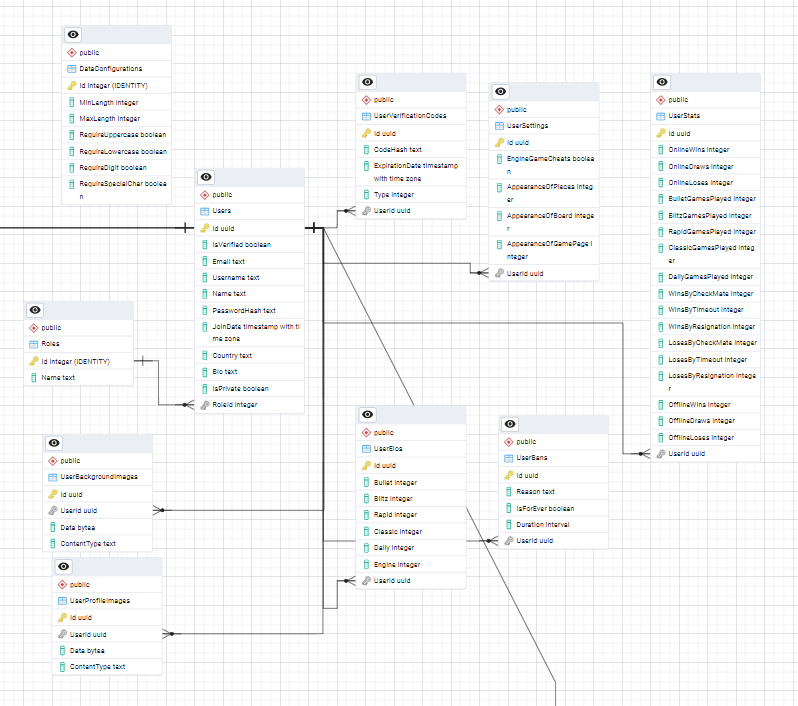
\includegraphics[width=0.8\textwidth]{zdj/user_ERD.png}
    \caption{Diagram relacji jednostka-relacja przedstawiający relacje użytkownika - wygenerowany za pomocą PgAdmin 4}
\end{figure}
\newpage

\noindent \textbf{Relacje znajomości} \\
Segment relacji przyjaźni jest zarządzany przez jednostkę przyjaźni, która reprezentuje połączenia społeczne między użytkownikami. Każda Encja Friendship ma dwóch kluczowych uczestników: Requestor (przyjmujacy) i Receiver (odbierający). Są to obaj użytkownicy, a relacje między tymi podmiotami są modelowane za pomocą kluczy obcych: RequestorId i ReceiverId. Ta relacja jest wiele-do-jednego, co oznacza, że użytkownik może mieć wiele przyjaźni zarówno jako żądający, jak i odbiorca. Dodatkowo, jednostka FriendshipStats śledzi statystyki związane z każdą przyjaźnią, tworząc relację jeden-do-jednego z jednostką Friendship.

\vspace{1cm}
\begin{figure}[h!]
    \centering
    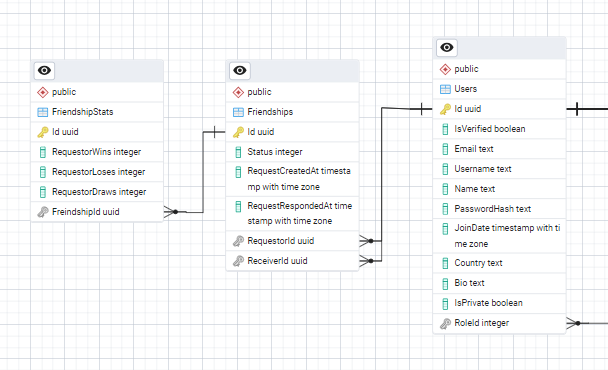
\includegraphics[width=0.8\textwidth]{zdj/friendship_ERD.png}
    \caption{Diagram relacji między podmiotami przedstawiający relacje przyjaźni między użytkownikami - wygenerowany za pomocą PgAdmin 4}
\end{figure}
\newpage

\noindent \textbf{Relacje w grach sieciowych} \\
Segment Web Game Relations obsługuje strukturę internetowej gry w szachy, z kilkoma jednostkami, które śledzą różne aspekty gry. Jednostka WebGame reprezentuje samą grę, łącząc graczy (WhitePlayer i BlackPlayer) poprzez relacje jeden-do-jednego. Stan i czas gry są kontrolowane przez encje WebGameState i WebGameTiming, które są połączone za pomocą kluczy obcych. Jednostka WebGamePlayer służy do śledzenia informacji specyficznych dla gracza dla każdej gry i odwołuje się do jednostki User. Ruchy wykonane w grze są przechowywane w encji WebGameMove, która ma relację wiele do jednego z WebGame. Dodatkowo, wiadomości wymieniane podczas gry są obsługiwane przez encje WebGameMessage i WebGamePlayerMessage, tworzące relacje odpowiednio z WebGame i WebGamePlayer.

\vspace{1cm}
\begin{figure}[h!]
    \centering
    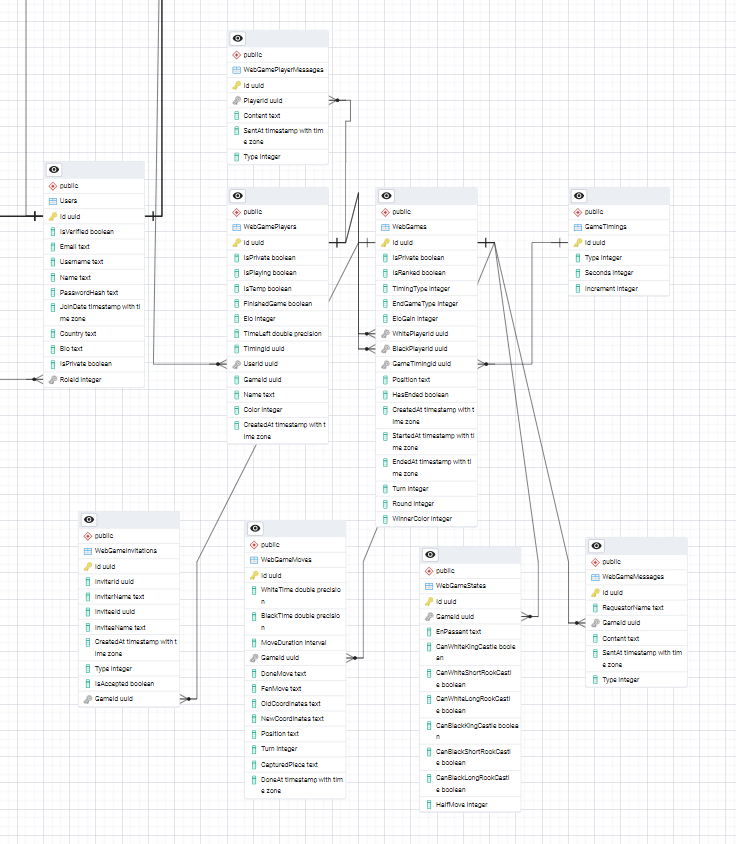
\includegraphics[width=0.8\textwidth]{zdj/online_ERD.png}
    \caption{Diagram relacji między podmiotami ilustrujący strukturę interakcji w grach sieciowych - wygenerowany za pomocą PgAdmin 4}
\end{figure}
\newpage

\noindent \textbf{Relacje w grach z silnikiem} \\
Segment ten skupia się na aspekcie gry opartym na silniku, gdzie każda gra jest zarządzana przez encję EngineGame. Encja EngineGame jest powiązana z encją EngineGamePlayer, reprezentującą użytkownika, który gra w grę opartą na silniku, a relacja jeden-do-jednego jest ustanawiana poprzez PlayerId. Każdy ruch w grze jest przechwytywany w encji EngineGameMove, która jest powiązana z encją EngineGame poprzez klucz obcy. Encja EngineGameState przechowuje aktualny stan gry opartej na silniku i jest powiązana z EngineGame poprzez relację jeden-do-jednego. Dodatkowo, wiadomości specyficzne dla gier silnikowych są przechowywane w encji EngineGameMessage, która jest powiązana z EngineGame poprzez klucz obcy.

\vspace{1cm}
\begin{figure}[h!]
    \centering
    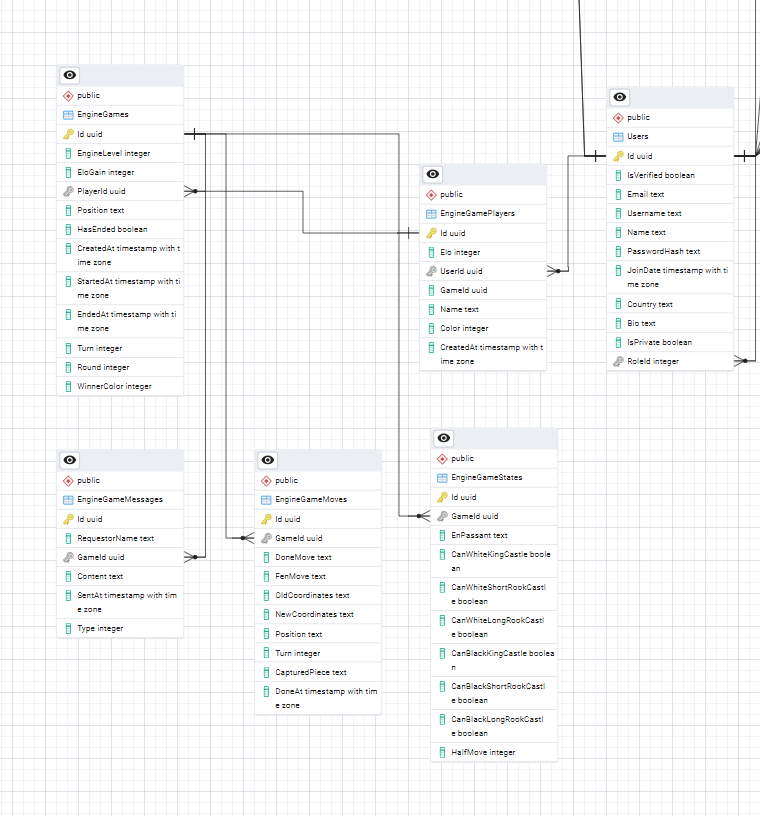
\includegraphics[width=0.8\textwidth]{zdj/offline_ERD.png}
    \caption{Diagram zależności między jednostkami przedstawiający relacje między silnikiem a grą - wygenerowany za pomocą PgAdmin 4}
\end{figure}
\newpage


\subsubsection{Opis encji}

\begin{itemize}
    \item \textbf{DataConfigurations} - Zawiera ustawienia konfiguracji dla kluczowych pól użytkownika.
    \begin{longtable}{|m{4cm}|m{2cm}|m{8cm}|}
        \hline
        \textbf{Właściwość} & \textbf{Typ} & \textbf{Opis} \\ \hline
        \endhead
        \hline
        Id & int & Identyfikator konfiguracji (PK) \\ \hline
        MinLength & int? & Minimalna długość pola \\ \hline
        MaxLength & int? & Maksymalna długość pola \\ \hline
        RequireUppercase & bool & Czy wymagana jest wielka litera \\ \hline
        RequireLowercase & bool & Czy wymagana jest mała litera \\ \hline
        RequireDigit & bool & Czy wymagana jest cyfra \\ \hline
        RequireSpecialChar & bool & Czy wymiany jest znak specjalny \\ \hline
    \end{longtable}

    \item \textbf{Roles} - Określa role użytkowników w systemie, takie jak "User" i "Admin".
    \begin{longtable}{|m{4cm}|m{2cm}|m{8cm}|}
        \hline
        \textbf{Właściwość} & \textbf{Typ} & \textbf{Opis} \\ \hline
        \endhead
        \hline
        Id & int & Identyfikator roli (PK) \\ \hline
        Name & string & Nazwa roli \\ \hline
    \end{longtable}

    \item \textbf{Users} - Główna encja reprezentująca użytkownika.
    \begin{longtable}{|m{4cm}|m{2cm}|m{8cm}|}
        \hline
        \textbf{Właściwość} & \textbf{Typ} & \textbf{Opis} \\ \hline
        \endhead
        \hline
        Id & Guid & Identyfikator użytkownika (PK) \\ \hline
        IsVerified & bool & Czy email użytkownika jest zweryfikowany \\ \hline
        Email & string & Adres email użytkownika \\ \hline
        Username & string & Unikalna nazwa użytkownika \\ \hline
        Name & string? & Pełne imię i nazwisko użytkownika \\ \hline
        PasswordHash & string & Zahashowane hasło użytkownika \\ \hline
        JoinDate & DateTime & Data dołączenia użytkownika do systemu \\ \hline
        Country & string & Kraj, w którym użytkownik się zarejestrował \\ \hline
        Bio & string? & Krótkie bio lub opis użytkownika \\ \hline
        IsPrivate & bool & Określa, czy profil użytkownika jest prywatny \\ \hline
        RoleId & int & Identyfikator roli użytkownika\\ \hline
    \end{longtable}

    \item \textbf{UserProfileImage} - zdjęcia profilowe użytkownika.
    \begin{longtable}{|m{4cm}|m{2cm}|m{8cm}|}
        \hline
        \textbf{Właściwość} & \textbf{Typ} & \textbf{Opis} \\ \hline
        \endhead
        \hline
        Id & Guid & Identyfikator obrazu użytkownika (PK) \\ \hline
        UserId & Guid & Identyfikator użytkownika do którego należy obraz \\ \hline
        Data & byte[] & Dane obrazu w postaci bajtów \\ \hline
        ContentType & string & Typ zawartości obrazu (np. "image/png", "image/jpeg") \\ \hline
    \end{longtable}
        
    \item \textbf{UserBackgroundImages} - tło profilu użytkownika.
    \begin{longtable}{|m{4cm}|m{2cm}|m{8cm}|}
        \hline
        \textbf{Właściwość} & \textbf{Typ} & \textbf{Opis} \\ \hline
        \endhead
        \hline
        Id & Guid & Identyfikator obrazu tła użytkownika (PK) \\ \hline
        UserId & Guid & Identyfikator użytkownika, do którego należy obraz tła \\ \hline
        Data & byte[] & Dane obrazu tła w postaci bajtów \\ \hline
        ContentType & string & Typ zawartości obrazu tła (np. "image/png", "image/jpeg") \\ \hline
    \end{longtable}
        
    \item \textbf{UserElos} - punktacja użytkownika dla poszczególnych trybów czasowych gry.
    \begin{longtable}{|m{4cm}|m{2cm}|m{8cm}|}
        \hline
        \textbf{Właściwość} & \textbf{Typ} & \textbf{Opis} \\ \hline
        \endhead
        \hline
        Id & Guid & Identyfikator ELO (PK) \\ \hline
        Bullet & int & Punkty ELO dla trybu Bullet \\ \hline
        Blitz & int & Punkty ELO dla trybu Blitz \\ \hline
        Rapid & int & Punkty ELO dla trybu Rapid \\ \hline
        Classic & int & Punkty ELO dla trybu Classic \\ \hline
        Daily & int & Punkty ELO dla trybu Daily \\ \hline
        Engine & int & Punkty ELO dla gier z silnikiem \\ \hline
        UserId & Guid & Identyfikator użytkownika, do którego należy ELO \\ \hline
    \end{longtable}
        
    \item \textbf{UserStats} - tablica statystyki użytkownika.
    \begin{longtable}{|m{4cm}|m{2cm}|m{8cm}|}
        \hline
        \textbf{Właściwość} & \textbf{Typ} & \textbf{Opis} \\ \hline
        \endhead
        \hline
        Id & Guid & Identyfikator statystyk użytkownika (PK) \\ \hline
        OnlineWins & int & Liczba wygranych gier online \\ \hline
        OnlineDraws & int & Liczba remisów gier online \\ \hline
        OnlineLoses & int & Liczba przegranych gier online \\ \hline
        OnlineGamesPlayed & int & Łączna liczba gier online \\ \hline
        BulletGamesPlayed & int & Liczba gier online w trybie Bullet \\ \hline
        BlitzGamesPlayed & int & Liczba gier online w trybie Blitz \\ \hline
        RapidGamesPlayed & int & Liczba gier online w trybie Rapid \\ \hline
        ClassicGamesPlayed & int & Liczba gier online w trybie Classic \\ \hline
        DailyGamesPlayed & int & Liczba gier online w trybie Daily \\ \hline
        WinsByCheckMate & int & Liczba wygranych przez mat \\ \hline
        WinsByTimeout & int & Liczba wygranych przez czas \\ \hline
        WinsByResignation & int & Liczba wygranych przez rezygnację \\ \hline
        LosesByCheckMate & int & Liczba przegranych przez mat \\ \hline
        LosesByTimeout & int & Liczba przegranych przez czas \\ \hline
        LosesByResignation & int & Liczba przegranych przez rezygnację \\ \hline
        OfflineWins & int & Liczba wygranych gier offline \\ \hline
        OfflineDraws & int & Liczba remisów gier offline \\ \hline
        OfflineLoses & int & Liczba przegranych gier offline \\ \hline
        OfflineGamesPlayed & int & Łączna liczba gier offline \\ \hline
        UserId & Guid & Identyfikator użytkownika, do którego należą statystyki \\ \hline
    \end{longtable}
        
    \item \textbf{UserSettings} - globalne ustawienia konta oraz gier.
    \begin{longtable}{|m{4cm}|m{2cm}|m{8cm}|}
        \hline
        \textbf{Właściwość} & \textbf{Typ} & \textbf{Opis} \\ \hline
        \endhead
        \hline
        Id & Guid & Identyfikator ustawień użytkownika (PK) \\ \hline
        EngineGameCheats & bool & Określa, czy oszustwa w grze silnikiem są dozwolone \\ \hline
        Ap-OfPieces & enum & Ustawienia wyglądu figur w grze \\ \hline
        Ap-OfBoard & enum & Ustawienia wyglądu planszy w grze \\ \hline
        Ap-OfGamePage & enum & Ustawienia wyglądu strony gry \\ \hline
        UserId & Guid & Identyfikator użytkownika, do którego należą ustawienia \\ \hline
    \end{longtable}

    \item \textbf{UserVerificationCodes} - tablica kodów weryfikacyjnych.
    \begin{longtable}{|m{4cm}|m{2cm}|m{8cm}|}
        \hline
        \textbf{Właściwość} & \textbf{Typ} & \textbf{Opis} \\ \hline
        \endhead
        \hline
        Id & Guid & Identyfikator kodu weryfikacyjnego (PK) \\ \hline
        CodeHash & string & Zahashowany kod używany do weryfikacji \\ \hline
        ExpirationDate & DateTime & Data wygaśnięcia kodu weryfikacyjnego \\ \hline
        Type & enum & Typ kodu weryfikacyjnego \\ \hline
        UserId & Guid & Identyfikator użytkownika, do którego należy kod weryfikacyjny \\ \hline
    \end{longtable}

    \item \textbf{Friendships} - tablica relacji pomiędzy użytkownikami.
    \begin{longtable}{|m{4cm}|m{2cm}|m{8cm}|}
        \hline
        \textbf{Właściwość} & \textbf{Typ} & \textbf{Opis} \\ \hline
        \endhead
        \hline
        Id & Guid & Identyfikator relacji przyjaźni (PK) \\ \hline
        Status & enum & Status przyjaźni  \\ \hline
        RequestCreatedAt & DateTime & Data utworzenia/złożenia wniosku o przyjaźń \\ \hline
        RequestRespondedAt & DateTime? & Data, kiedy druga strona odpowiedziała na wniosek o przyjaźń \\ \hline
        RequestorId & Guid & Identyfikator użytkownika, który wysłał prośbę o przyjaźń \\ \hline
        ReceiverId & Guid & Identyfikator użytkownika, który otrzymał prośbę o przyjaźń \\ \hline
    \end{longtable}
        
  
    \item \textbf{FriendshipStats} - Statystki dotyczące relacji uzytkownikow.
    \begin{longtable}{|m{4cm}|m{2cm}|m{8cm}|}
        \hline
        \textbf{Właściwość} & \textbf{Typ} & \textbf{Opis} \\ \hline
        \endhead
        \hline
        Id & Guid & Identyfikator statystyk przyjaźni (PK) \\ \hline
        RequestorWins & int & Liczba wygranych przez osobę, która wysłała prośbę o przyjaźń \\ \hline
        RequestorLoses & int & Liczba przegranych przez osobę, która wysłała prośbę o przyjaźń \\ \hline
        RequestorDraws & int & Liczba remisów osoby, która wysłała prośbę o przyjaźń \\ \hline
        GamesPlayed & int & Łączna liczba rozegranych gier w relacji \\ \hline
        FriendshipId & Guid & Identyfikator relacji przyjaźni, do której należą statystyki \\ \hline
    \end{longtable}
        
    \item \textbf{WebGames} - Gry online między użytkownikami.
    \begin{longtable}{|m{4cm}|m{2cm}|m{8cm}|}
        \hline
        \textbf{Właściwość} & \textbf{Typ} & \textbf{Opis} \\ \hline
        \endhead
        \hline
        Id & Guid & Identyfikator gry online (PK) \\ \hline
        IsPrivate & bool & Określa, czy gra jest prywatna czy publiczna \\ \hline
        IsRanked & bool & Określa, czy gra będzie miała wpływ na ranking Elo \\ \hline
        TimingType & enum & Typ czasu gry (np. Bullet, Blitz, Rapid) \\ \hline
        EndGameType & enum? & Powód zakończenia gry (np. mat, czas) \\ \hline
        EloGain & int & Zysk lub strata Elo po zakończeniu gry \\ \hline
        WhitePlayerId & Guid & Identyfikator gracza grającego białymi \\ \hline
        BlackPlayerId & Guid & Identyfikator gracza grającego czarnymi \\ \hline
        GameTimingId & Guid & Identyfikator ustawień czasu gry \\ \hline
        Position & string & Aktualna pozycja na szachownicy \\ \hline
        HasEnded & bool & Flaga, czy gra się zakończyła \\ \hline
        CreatedAt & DateTime & Data utworzenia gry \\ \hline
        StartedAt & DateTime? & Data rozpoczęcia gry \\ \hline
        EndedAt & DateTime? & Data zakończenia gry \\ \hline
        Turn & int & Numer tury gry \\ \hline
        Round & int & Numer rundy \\ \hline
        WinnerColor & enum? & Kolor zwycięzcy (null oznacza remis) \\ \hline
    \end{longtable}
        
        
 
    \item \textbf{GameTimings} - kontrole czasowe dla gier z ograniczeniem czasu.
    \begin{longtable}{|m{4cm}|m{2cm}|m{8cm}|}
        \hline
        \textbf{Właściwość} & \textbf{Typ} & \textbf{Opis} \\ \hline
        \endhead
        \hline
        Id & Guid & Identyfikator ustawienia czasu gry (PK) \\ \hline
        Type & enum & Typ czasu (np. Bullet, Rapid) \\ \hline
        Seconds & int & Czas trwania gry w sekundach \\ \hline
        Increment & int & Inkrement czasowy w sekundach \\ \hline
    \end{longtable}
        

    \item \textbf{WebGameStates} - Stan gry online, przechowuje dane szczególne dotyczące obecnej gry.
    \begin{longtable}{|m{4cm}|m{2cm}|m{8cm}|}
        \hline
        \textbf{Właściwość} & \textbf{Typ} & \textbf{Opis} \\ \hline
        \endhead
        \hline
        Id & Guid & Identyfikator stanu gry (PK) \\ \hline
        GameId & Guid & Identyfikator gry, do której należy stan \\ \hline
        EnPassant & string? & Koordynaty dla ruchu en passant w formacie x,y \\ \hline
        CWKing & bool & Czy biały król może jeszcze wykonać roszadę \\ \hline
        CWShort & bool & Czy biały król może wykonać krótką roszadę \\ \hline
        CWLong & bool & Czy biały król może wykonać długą roszadę \\ \hline
        CBKing & bool & Czy czarny król może jeszcze wykonać roszadę \\ \hline
        CBShort & bool & Czy czarny król może wykonać krótką roszadę \\ \hline
        CBLong & bool & Czy czarny król może wykonać długą roszadę \\ \hline
        HalfMove & int & Liczba ruchów nie będących ruchem pionkiem (dla zasady 50 ruchów) \\ \hline
    \end{longtable}
        

    \item \textbf{WebGameInvitations} - Opcjonalne zaproszenia do gry.
    \begin{longtable}{|m{4cm}|m{2cm}|m{8cm}|}
        \hline
        \textbf{Właściwość} & \textbf{Typ} & \textbf{Opis} \\ \hline
        \endhead
        \hline
        Id & Guid & Identyfikator zaproszenia (PK) \\ \hline
        InviterId & Guid & Identyfikator użytkownika zapraszającego \\ \hline
        InviterName & string & Nazwa użytkownika zapraszającego \\ \hline
        InviteeId & Guid & Identyfikator użytkownika zapraszanego \\ \hline
        InviteeName & string & Nazwa użytkownika zapraszanego \\ \hline
        CreatedAt & DateTime & Data utworzenia zaproszenia \\ \hline
        Type & enum & Typ czasu gry, do którego odnosi się zaproszenie \\ \hline
        IsAccepted & bool & Flaga, która wskazuje, czy zaproszenie zostało zaakceptowane \\ \hline
        GameId & Guid & Identyfikator gry, do której zaproszenie należy \\ \hline
    \end{longtable}
        

    \item \textbf{WebGameMessages} - Wiadomości systemowe dotyczące gry online.
    \begin{longtable}{|m{4cm}|m{2cm}|m{8cm}|}
        \hline
        \textbf{Właściwość} & \textbf{Typ} & \textbf{Opis} \\ \hline
        \endhead
        \hline
        Id & Guid & Identyfikator wiadomości (PK) \\ \hline
        RequestorName & string & Nazwa użytkownika, który zażądał remisu \\ \hline
        GameId & Guid & Identyfikator gry, do której wiadomość należy \\ \hline
        Content & string & Treść wiadomości \\ \hline
        SentAt & DateTime & Data i godzina wysłania wiadomości \\ \hline
        Type & enum & Typ wiadomości (np. prośba o remis) \\ \hline
    \end{longtable}
        

    \item \textbf{WebGameMove} - Ruchy wykonane podczas gry online.
    \begin{longtable}{|m{4cm}|m{2cm}|m{8cm}|}
        \hline
        \textbf{Właściwość} & \textbf{Typ} & \textbf{Opis} \\ \hline
        \endhead
        \hline
        Id & Guid & Identyfikator ruchu (PK) \\ \hline
        WhiteTime & double & Czas pozostały dla białego gracza \\ \hline
        BlackTime & double & Czas pozostały dla czarnego gracza \\ \hline
        MoveDuration & TimeSpan & Czas, który gracz zużył na wykonanie ruchu \\ \hline
        GameId & Guid & Identyfikator gry, do której ruch należy \\ \hline
        DoneMove & string & Wykonany ruch w formacie: tag figury + x (jeśli zbicie) + współrzędne xy \\ \hline
        FenMove & string & Wykonany ruch w formacie FEN \\ \hline
        OldCoordinates & string & Współrzędne, z których figura została przemieszczona w formacie x,y \\ \hline
        NewCoordinates & string & Współrzędne, na które figura została przemieszczona w formacie x,y \\ \hline
        Position & string & Pozycja na szachownicy po wykonaniu ruchu \\ \hline
        Turn & int & Tura, w której ruch został wykonany \\ \hline
        CapturedPiece & string? & Tag zbitej figury \\ \hline
        DoneAt & DateTime & Data i godzina wykonania ruchu \\ \hline
    \end{longtable}
        
    \item \textbf{WebGamePlayers} - Tablica graczy gry online.
    \begin{longtable}{|m{4cm}|m{2cm}|m{8cm}|}
        \hline
        \textbf{Właściwość} & \textbf{Typ} & \textbf{Opis} \\ \hline
        \endhead
        \hline
        Id & Guid & Identyfikator gracza (PK) \\ \hline
        IsPrivate & bool & Określa, czy gracz może być używany w globalnym wyszukiwaniu, czy jest tylko dla prywatnej gry \\ \hline
        IsPlaying & bool & Flaga, czy gracz wciąż szuka gry \\ \hline
        IsTemp & bool & Flaga, czy gracz jest tymczasowy \\ \hline
        FinishedGame & bool & Flaga, czy gra dla gracza została zakończona \\ \hline
        Elo & int & Punkty Elo dla konkretnego typu czasu \\ \hline
        TimeLeft & double & Czas pozostały na wykonanie ruchów zgodnie z czasem gry \\ \hline
        TimingId & Guid & Identyfikator typu czasu, określający czas trwania i przyrost czasu dla wszystkich ruchów \\ \hline
        UserId & Guid & Identyfikator użytkownika, któremu gracz należy \\ \hline
        GameId & Guid & Identyfikator gry, w której gracz bierze udział \\ \hline
        Name & string & Nazwa gracza (nazwa użytkownika) \\ \hline
        Color & enum? & Kolor gracza (czarny lub biały), null jeśli gracz szuka jeszcze gry \\ \hline
        CreatedAt & DateTime & Data utworzenia gracza \\ \hline
    \end{longtable}

    \item \textbf{WebGamePlayerMessages} - wiadomości wysłane przez graczy podczas gry online.
    \begin{longtable}{|m{4cm}|m{2cm}|m{8cm}|}
        \hline
        \textbf{Właściwość} & \textbf{Typ} & \textbf{Opis} \\ \hline
        \endhead
        \hline
        Id & Guid & Identyfikator wiadomości (PK) \\ \hline
        PlayerId & Guid & Identyfikator gracza, który wysłał wiadomość \\ \hline
        Content & string & Treść wiadomości \\ \hline
        SentAt & DateTime & Data i czas wysłania wiadomości \\ \hline
        Type & enum & Typ wiadomości \\ \hline
    \end{longtable}
        
    \item \textbf{EngineGames} - Tablica gier offline z silnikiem szachowym. 
    \begin{longtable}{|m{4cm}|m{2cm}|m{8cm}|}
        \hline
        \textbf{Właściwość} & \textbf{Typ} & \textbf{Opis} \\ \hline
        \endhead
        \hline
        Id & Guid & Identyfikator gry (PK) \\ \hline
        EngineLevel & int & Poziom głębokości silnika \\ \hline
        EloGain & int & Zysk lub strata Elo po zakończeniu gry \\ \hline
        PlayerId & Guid & Identyfikator gracza \\ \hline
        Position & string & Aktualna pozycja w grze \\ \hline
        HasEnded & bool & Flaga informująca, czy gra zakończona \\ \hline
        CreatedAt & DateTime & Data utworzenia gry \\ \hline
        StartedAt & DateTime? & Data rozpoczęcia gry \\ \hline
        EndedAt & DateTime? & Data zakończenia gry \\ \hline
        Turn & int & Numer tury gry \\ \hline
        Round & int & Numer rundy gry (pełny ruch) \\ \hline
        WinnerColor & enum? & Kolor zwycięzcy (null oznacza remis) \\ \hline
    \end{longtable}

    
    \item \textbf{EngineGameStates} - Stan gry offline, przechowuje dane szczególne dotyczące obecnej gry.
    \begin{longtable}{|m{4cm}|m{2cm}|m{8cm}|}
        \hline
        \textbf{Właściwość} & \textbf{Typ} & \textbf{Opis} \\ \hline
        \endhead
        \hline
        Id & Guid & Identyfikator stanu gry (PK) \\ \hline
        GameId & Guid & Identyfikator gry, do której należy stan \\ \hline
        EnPassant & string? & Współrzędne en passant, jeśli możliwe, w formacie x,y \\ \hline
        CWKing & bool & Czy biały król może jeszcze wykonać roszadę \\ \hline
        CWShort & bool & Czy biały król może wykonać krótką roszadę \\ \hline
        CWLong & bool & Czy biały król może wykonać długą roszadę \\ \hline
        CBKing & bool & Czy czarny król może jeszcze wykonać roszadę \\ \hline
        CBShort & bool & Czy czarny król może wykonać krótką roszadę \\ \hline
        CBLong & bool & Czy czarny król może wykonać długą roszadę \\ \hline
        HalfMove & int & Liczba ruchów wykonanych przez graczy, z wyjątkiem pionków, dla zasady 50 ruchów \\ \hline
    \end{longtable}
    

    \item \textbf{EngineGamePlayers} - Gracze gier offline.
    \begin{longtable}{|m{4cm}|m{2cm}|m{8cm}|}
        \hline
        \textbf{Właściwość} & \textbf{Typ} & \textbf{Opis} \\ \hline
        \endhead
        \hline
        Id & Guid & Identyfikator gracza (PK) \\ \hline
        Elo & int & Punkty Elo dla gier przeciwko silnikowi \\ \hline
        UserId & Guid & Identyfikator użytkownika, do którego należy gracz \\ \hline
        GameId & Guid & Identyfikator gry, w której gracz bierze udział \\ \hline
        Name & string & Nazwa użytkownika (imię gracza) \\ \hline
        Color & enum? & Kolor gracza (czarny lub biały), null oznacza oczekiwanie na grę \\ \hline
        CreatedAt & DateTime & Data utworzenia gracza (do kolejek oczekujących) \\ \hline
    \end{longtable}
    
    \item \textbf{EngineGameMoves} - Ruchy wykonane podczas gry offline.
    \begin{longtable}{|m{4cm}|m{2cm}|m{8cm}|}
        \hline
        \textbf{Właściwość} & \textbf{Typ} & \textbf{Opis} \\ \hline
        \endhead
        \hline
        Id & Guid & Identyfikator ruchu (PK) \\ \hline
        GameId & Guid & Identyfikator gry, do której należy ruch \\ \hline
        DoneMove & string & Wykonany ruch w formacie: oznaczenie figury + x (jeśli zbicie) + współrzędne xy \\ \hline
        FenMove & string & Wykonany ruch w formacie FEN \\ \hline
        OldCoordinates & string & Współrzędne, z których figura została przesunięta (format "x,y") \\ \hline
        NewCoordinates & string & Współrzędne, na które figura została przesunięta (format "x,y") \\ \hline
        Position & string & Pozycja po wykonaniu ruchu \\ \hline
        Turn & int & Tura, w której wykonano ruch \\ \hline
        CapturedPiece & string? & Zbita figura, jeśli dotyczy \\ \hline
        DoneAt & DateTime & Data i godzina wykonania ruchu \\ \hline
    \end{longtable}
    
    \item \textbf{EngineGameMessages} - Automatyczne wiadomości dotyczące gry offline.
    \begin{longtable}{|m{4cm}|m{2cm}|m{8cm}|}
        \hline
        \textbf{Właściwość} & \textbf{Typ} & \textbf{Opis} \\ \hline
        \endhead
        \hline
        Id & Guid & Identyfikator wiadomości (PK) \\ \hline
        RequestorName & string & Nazwa osoby lub systemu wysyłającego wiadomość (domyślnie "BRN CHess") \\ \hline
        GameId & Guid & Identyfikator gry, do której należy wiadomość \\ \hline
        Content & string & Treść wiadomości \\ \hline
        SentAt & DateTime & Data i godzina wysłania wiadomości \\ \hline
        Type & enum & Typ wiadomości \\ \hline
    \end{longtable}
    
\end{itemize}

\newpage
\subsection{Backend} 
\subsubsection{Architektura} 
Architektura backendu została zaprojektowana w oparciu o podejście Onion Architecture, które promuje modularność, odwrócenie zależności oraz izolację logiki biznesowej od infrastruktury. Główne założenia tej architektury koncentrują się na umożliwieniu rozwoju aplikacji w sposób niezależny od technologii, co sprzyja łatwemu utrzymaniu oraz skalowaniu systemu. Struktura projektu jest podzielona na kilka warstw, które komunikują się ze sobą poprzez jasno zdefiniowane kontrakty i interfejsy. Kluczowym celem tego podejścia jest ochrona rdzenia aplikacji przed zmianami w zewnętrznych technologiach i zależnościach, co pozwala na łatwiejsze dostosowywanie aplikacji do nowych wymagań i technologii.


\begin{figure}[h!] 
    \centering 
    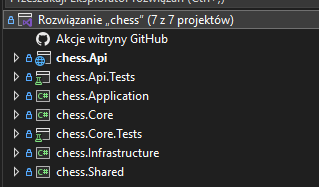
\includegraphics[width=0.7\textwidth]{zdj/struktura_back.png} 
    \caption{Struktura projektów solucji.} 
\end{figure}

Zalety Onion Architecture to:
\begin{itemize}
    \item \textbf{Izolacja logiki biznesowej:} pozwala na pełną separację logiki biznesowej od zewnętrznych zależności, co umożliwia łatwe testowanie i modyfikowanie samej logiki bez wpływu na resztę systemu.
    \item \textbf{Skalowalność i elastyczność:} modularność struktury pozwala na łatwą rozbudowę systemu, poprzez dodawanie nowych warstw lub rozszerzanie istniejących komponentów bez ryzyka wprowadzenia chaosu w kodzie.
    \item \textbf{Testowalność:} dzięki wyodrębnieniu warstw odpowiedzialnych za różne aspekty systemu, testowanie staje się prostsze i bardziej zorganizowane, ponieważ możemy testować poszczególne warstwy niezależnie.
    \item \textbf{Odwrócenie zależności:} warstwa zewnętrzna może korzystać z funkcjonalności warstw wewnętrznych, ale nie odwrotnie. To oznacza, że zmiany w bazach danych czy frameworkach nie wpływają na kluczową logikę biznesową aplikacji.
\end{itemize}

Podejście to pozwala na przejrzystość w organizacji kodu, ułatwiając zarządzanie projektem i współpracę zespołową. Dzięki jasnemu podziałowi na warstwy, każdy członek zespołu może skupić się na odpowiednim obszarze aplikacji, bez konieczności przyswajania całościowej struktury systemu. Dodatkowo, umożliwia łatwe przeprowadzanie migracji technologicznych w obrębie poszczególnych warstw, minimalizując ryzyko wprowadzenia błędów w działającej aplikacji.

\newpage

Zależności między poszczególnymi modułami zaprezentowane zostały za pomocą grafu, co pozwala na wizualizację i lepsze zrozumienie interakcji między warstwami. Graf ten odzwierciedla zasady Onion Architecture, w której zależności zawsze kierują się do wewnątrz, tj. od warstw zewnętrznych do bardziej wewnętrznych.
\\\\
Moduł .Api zależy wyłącznie od warstwy .Application, co oznacza, że obsługuje żądania i deleguje ich przetwarzanie do przypadków użycia w Application. Z kolei .Application komunikuje się z modułem .Core, który definiuje kluczowe modele domenowe. Warstwa .Core pozostaje całkowicie niezależna od innych modułów, co jest zgodne z zasadami odwrócenia zależności.
\\
Moduł .Infrastructure implementuje interfejsy zdefiniowane w .Application, dostarczając szczegóły techniczne, takie jak integracje czy dostęp do danych, ale nie wymusza zależności zwrotnej na rdzeniu. .Shared działa jako pomocniczy moduł, który może być używany przez dowolną warstwę, dostarczając wspólny kod i narzędzia.

\begin{figure}[h!]
    \centering
    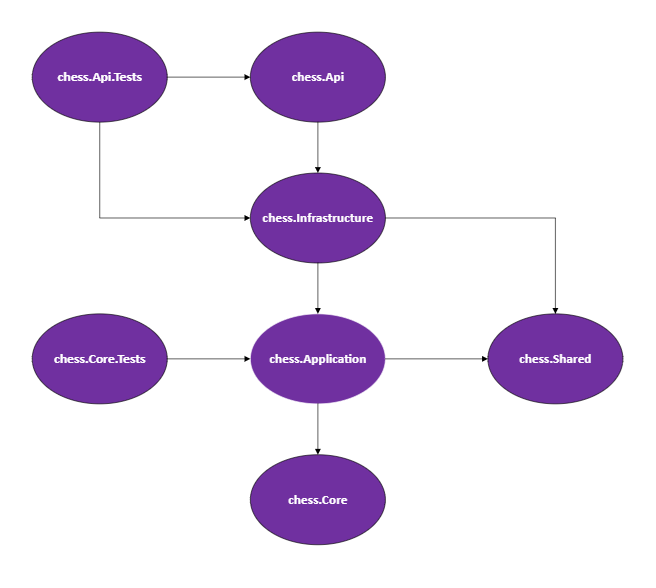
\includegraphics[width=1\textwidth]{zdj/backend_dependencies.png}
    \caption{Graf zależności między projektami}
\end{figure}

\newpage

\textbf{Warstwa prezentacji}\\
Moduł .Api pełni funkcję warstwy zewnętrznej, odpowiedzialnej za obsługę żądań HTTP oraz przekazywanie ich do odpowiednich komponentów logiki aplikacji. Jest to punkt wejściowy dla użytkowników lub zewnętrznych integracji. Warstwa ta korzysta z usług dostarczanych przez moduł Application, pozostając przy tym niezależna od szczegółów implementacyjnych niższych warstw.

\vspace{0.5cm}
\begin{minipage}[t]{0.45\textwidth}
    \vspace{0pt}
    \raggedright
    Warstwa prezentacji odpowiada za obsługę komunikacji zewnętrznej aplikacji, interpretację żądań od użytkowników oraz ich przekazywanie do warstw logiki aplikacyjnej. Zawiera kontrolery realizujące logikę obsługi poszczególnych zasobów oraz huby, takie jak SignalR Hub, które obsługują komunikację w czasie rzeczywistym. Modele w tym module reprezentują dane odbierane z endpointów aplikacji. Mapy przekształcają te modele na żądania odpowiadające wymaganiom warstwy aplikacyjnej. Moduł zapewnia również mechanizmy autoryzacji, umożliwiające kontrolę dostępu do zasobów i operacji w systemie.
\end{minipage}
\hfill
\begin{minipage}[t]{0.45\textwidth}
    \vspace{0pt}
    \centering
    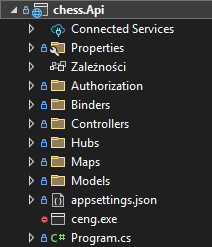
\includegraphics[width=\linewidth]{zdj/struktura_back_api.png}
\end{minipage}
\vspace{0.5cm}

\textbf{Warstwa aplikacji}\\
Moduł .Application zawiera logikę aplikacyjną, w tym definicje przypadków użycia (use cases), które realizują wymagania systemowe. Jest on pośrednikiem między warstwą interfejsu (Api) a rdzeniem systemu, reprezentowanym przez moduł .Core. Dzięki temu logika biznesowa jest chroniona przed szczegółami technicznymi, takimi jak sposób przetwarzania żądań czy dostęp do danych.

\vspace{0.5cm}
\begin{minipage}[t]{0.45\textwidth}
    \vspace{0pt}
    \centering
    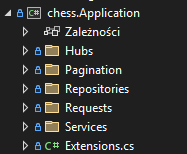
\includegraphics[width=\linewidth]{zdj/struktura_back_application.png} 
\end{minipage}
\hfill
\begin{minipage}[t]{0.45\textwidth}
    \vspace{0pt}
    \raggedright
    Warstwa aplikacji łączy warstwy zewnętrzne z rdzeniem systemu. Zawiera interfejsy dla hubów SignalR (Hubs), repozytoriów (Repositories) i usług (Services), definiujące kluczowe kontrakty. W Requests znajdują się żądania obsługiwane przez MediatR, wspierające wzorzec CQRS. Moduł Pagination dostarcza abstrakcje do paginacji wyników, istotne przy operacjach na dużych zbiorach danych.
\end{minipage}
\vspace{0.5cm}

\textbf{Warstwa dostępu do danych}\\
Moduł .Infrastructure obsługuje szczegóły techniczne, takie jak dostęp do bazy danych, integracje z zewnętrznymi usługami czy komunikacja z innymi systemami. Implementuje on interfejsy zdefiniowane w .Core, zapewniając zgodność z wymogami logiki biznesowej. Dzięki temu warstwa infrastrukturalna może być łatwo modyfikowana lub wymieniana bez wpływu na działanie innych części aplikacji.

\vspace{0.5cm}
\begin{minipage}[t]{0.45\textwidth}
    \vspace{0pt}
    \raggedright
    Warstwa infrastruktury zawiera kluczowe elementy zarządzania danymi i konfiguracji aplikacji. W folderze Contexts znajduje się klasa kontekstu bazy danych, która mapuje encje aplikacji na tabele. W Configuration zapisane są relacje między encjami oraz konfiguracja ich mapowania. Foldery Services i Repositories zawierają implementacje interfejsów zdefiniowanych w warstwie aplikacji, które odpowiadają za dostęp do danych. Workers to klasy odpowiedzialne za zadania cykliczne działające w tle. Migrations natomiast zawiera skrypty migracji bazy danych, umożliwiające zarządzanie zmianami w schemacie bazy danych.
\end{minipage}
\hfill
\begin{minipage}[t]{0.45\textwidth}
    \vspace{0pt}
    \centering
    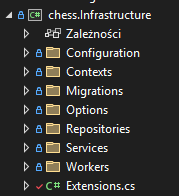
\includegraphics[width=\linewidth]{zdj/struktura_back_infrastructure.png} 
\end{minipage}
\vspace{0.5cm}

\textbf{Warstwa logiki biznesowej}\\
Moduł .Core stanowi serce aplikacji i zawiera jej logikę biznesową oraz kluczowe modele domenowe. Jest to najbardziej niezależna warstwa, która nie zna szczegółów implementacyjnych zewnętrznych warstw. Wszystkie zależności są odwrócone – moduł .Core definiuje interfejsy, które są implementowane przez warstwę infrastrukturalną, co pozwala na łatwą wymianę technologii bez wpływu na rdzeń aplikacji.

\vspace{0.5cm}
\begin{minipage}[t]{0.45\textwidth}
    \vspace{0pt}
    \centering
    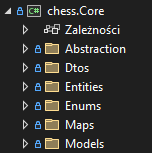
\includegraphics[width=\linewidth]{zdj/struktura_back_core.png} 
\end{minipage}
\hfill
\begin{minipage}[t]{0.45\textwidth}
    \vspace{0pt}
    \raggedright
    Warstwa domenowa stanowi fundament aplikacji, zawierając kluczowe definicje i logikę biznesową. W folderze Entities znajdują się główne encje, które odpowiadają za przechowywanie danych w systemie. Enums zawiera wyliczenia, które definiują stałe wartości. W Abstractions znajdują się abstrakcyjne klasy, które są dziedziczone przez podobne encje. Dtos zawiera obiekty transferu danych zwracane przez zapytania, w tym często wykorzystywane DTO, które są dzielone pomiędzy różnymi zapytaniami. Models przechowuje wspólne modele używane przez różne procesy. W Maps znajduje się logika mapowania danych w postaci słownika, który definiuje operacje pobierania, ustawiania i aktualizowania wartości w encjach..
\end{minipage}
\vspace{0.5cm}

\textbf{Warstwa wspólna }\\
Moduł .Shared zawiera wspólne komponenty i funkcjonalności, które są wykorzystywane przez inne warstwy aplikacji. Celem tej warstwy jest centralizacja użytecznych elementów, które nie są specyficzne dla jednej warstwy, a są wykorzystywane przez różne części systemu. Dzięki temu wspólne elementy, takie jak wyjątki, middleware oraz konfiguracje, są łatwo dostępne, a zarządzanie nimi jest uproszczone. Warstwa ta pełni rolę wspierającą, zapewniając rozwiązania, które mogą być współdzielone przez inne warstwy aplikacji, co zwiększa spójność i ułatwia konserwację systemu.

\begin{minipage}[t]{0.45\textwidth}
    \vspace{0pt}
    \raggedright
    Warstwa wspólna .Shared zawiera wspólne komponenty, które są wykorzystywane przez inne warstwy aplikacji. Folder Exceptions przechowuje wyjątki, które pozwalają na precyzyjne zarządzanie błędami w systemie. Middleware zawiera komponenty pośredniczące, które przechwytują i obsługują błędy HTTP, zapewniając odpowiednie kody statusu oraz komunikaty w odpowiedzi. W folderze Options znajdują się rozszerzenia umożliwiające łatwe pobieranie konfiguracji z pliku appsettings, co zapewnia centralne zarządzanie ustawieniami aplikacji.
\end{minipage}
\hfill
\begin{minipage}[t]{0.45\textwidth}
    \vspace{0pt}
    \centering
    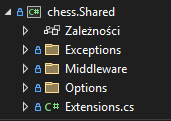
\includegraphics[width=\linewidth]{zdj/struktura_back_shared.png} 
\end{minipage}
\vspace{0.5cm}

\textbf{Warstwa testów integracyjnych}\\
Moduł .Api.Tests zawiera testy integracyjne dla kontrolerów API, zapewniając weryfikację poprawności działania interfejsu API w kontekście integracji z innymi komponentami systemu, takimi jak baza danych czy logika aplikacyjna. Testy te sprawdzają, czy odpowiedzi API są zgodne z oczekiwaniami, weryfikując m.in. poprawność danych wejściowych i wyjściowych oraz obsługę błędów. Każdy folder w tym module odpowiada pojedynczemu kontrolerowi API, umożliwiając modularne testowanie poszczególnych elementów aplikacji. Dzięki testom integracyjnym możliwe jest sprawdzenie, czy aplikacja poprawnie reaguje na różnorodne scenariusze i przypadki brzegowe.

\vspace{0.5cm}
\begin{minipage}[t]{0.45\textwidth}
    \vspace{0pt}
    \centering
    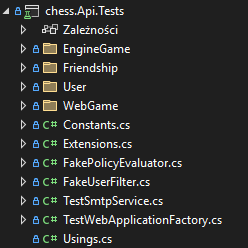
\includegraphics[width=\linewidth]{zdj/struktura_back_api_tests.png} 
\end{minipage}
\hfill
\begin{minipage}[t]{0.45\textwidth}
    \vspace{0pt}
    \raggedright
    Warstwa .Api.Tests zawiera testy integracyjne dla kontrolerów API. Każdy folder w tej warstwie odpowiada jednemu kontrolerowi API, umożliwiając modularne testowanie różnych części aplikacji. Testy wykorzystują narzędzia takie jak FluentAssertions i XUnit do tworzenia środowiska testowego. Testy te sprawdzają integrację kontrolera API z bazą danych oraz logiką aplikacyjną, testując poprawne działanie czy obsługę błędów w przypadku niepoprawnych danych wejściowych.
\end{minipage}
\vspace{0.5cm}

\textbf{Warstwa testów logiki biznesowej}\\
Moduł .Core.Tests zawiera testy jednostkowe dla logiki biznesowej aplikacji. Testy te weryfikują poprawność działania poszczególnych komponentów wewnętrznych systemu, takich jak handled żądań, serwisy, repozytoria oraz inne elementy logiki biznesowej. Dzięki tym testom możliwe jest zapewnienie, że logika aplikacji działa zgodnie z wymaganiami, niezależnie od zewnętrznych zależności. Testy jednostkowe pozwalają na szybsze i łatwiejsze identyfikowanie błędów w samej logice aplikacji, zanim zmiany wpłyną na inne warstwy systemu.

\vspace{0.5cm}
\begin{minipage}[t]{0.45\textwidth}
    \vspace{0pt}
    \raggedright
    Warstwa .Core.Tests zawiera testy jednostkowe dla logiki biznesowej aplikacji. Testy są podzielone na foldery odpowiadające poszczególnym kontrolerom. Celem tych testów jest weryfikacja poprawności działania komponentów aplikacji, takich jak handlerów żądań, serwisów, czy repozytoriów. Testy skupiają się na sprawdzeniu logiki biznesowej, walidacji danych, oraz obsługi wyjątków, wykorzystując narzędzia takie jak mocki, aby izolować testowane jednostki od zewnętrznych zależności. Dzięki temu możliwe jest testowanie samej logiki aplikacji bez potrzeby uruchamiania pełnej infrastruktury.
\end{minipage}
\hfill
\begin{minipage}[t]{0.45\textwidth}
    \vspace{0pt}
    \centering
    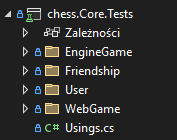
\includegraphics[width=\linewidth]{zdj/struktura_back_core_tests.png} 
\end{minipage}
\vspace{0.5cm}



\newpage
\subsubsection{REST API}

Interfejsy API są najpopularniejszym sposobem interakcji programów i urządzeń w nowoczesnych technologiach obliczeniowych. API to zestaw reguł opisujących, jak jeden program może się łączyć oraz komunikować z innym. Jak sama nazwa wskazuje, API REST przekazuje na każde żądanie stan każdej transakcji, co daje korzyści związane z opracowaniem, wydajnością i zasobami w porównaniu do innych metod. REST rozwija się w ciągu ponad dwóch dekad i jest bardzo powszechnym podejściem do architektur opartych na usługach i architektur rozproszonych.
\\\\
Zasób jest podstawowym pojęciem dla API REST. Zasób jest obiektem, który ma typ, powiązane dane, relacje z innymi zasobami i zestaw metod, które na nim działają. Jest bardzo podobny do idei obiektów w programowaniu, chociaż zdefiniowanych jest tylko kilka standardowych metod, typowych dla HTTP GET, POST, PUT i DELETE. Zasoby mogą istnieć same lub w zbiorach, które same są zasobami.
\\\\
W nowoczesnej informatyce wspólnym modelem - również podstawowym dla API REST - jest klient-serwer, gdzie klient, który potrzebuje zasobu, identyfikuje się i komunikuje z serwerem, który może go dostarczyć. W ten sposób zarządzany jest praktycznie cały ruch w chmurze, gdyż oferuje maksymalną elastyczność licznym klientom i pozwala na dostęp do licznych serwerów. Zasada ta sprawdza się również w przypadku tzw. architektur „bezserwerowych", w których miejsce serwera znanego klientowi zajmuje broker usług.

\newpage

\textbf{Endpointy}
\begin{itemize}
    \item \textbf{UserController}
    \begin{itemize} 
        \item \textbf{POST /api/user/sign-up} - Rejestruje użytkownika i wysyła kod weryfikacyjny e-mailem. 
        \item \textbf{POST /api/user/sign-in} - Loguje użytkownika i generuje token JWT. 
        \item \textbf{POST /api/user/regenerate-code} - Generuje nowy kod weryfikacyjny, usuwając stary, dla użytkowników, którzy jeszcze nie zweryfikowali swojego konta. 
        \item \textbf{PUT /api/user/verify-email} - Weryfikuje adres e-mail użytkownika za pomocą dostarczonego kodu. 
        \item \textbf{PUT /api/user/send-password-code} - Wysyła kod weryfikacyjny do odzyskania hasła. 
        \item \textbf{PUT /api/user/reset-password} - Resetuje hasło użytkownika po podaniu kodu weryfikacyjnego. 
        \item \textbf{PUT /api/user/change-password} - Zmienia hasło użytkownika, dostępne tylko dla użytkowników, którzy są zalogowani i zweryfikowani. 
        \item \textbf{PUT /api/user/profile} - Aktualizuje dane profilu użytkownika. 
        \item \textbf{PUT /api/user/data} - Zmienia dane użytkownika, takie jak imię, nazwisko itp. 
        \item \textbf{PUT /api/user/settings} - Zmienia ustawienia użytkownika, np. preferencje konta. 
        \item \textbf{GET /api/user} - Pobiera podstawowe informacje o użytkowniku. 
        \item \textbf{GET /api/user/full} - Pobiera pełne informacje o użytkowniku, takie jak historia, rankingi, szczegóły profilu. 
        \item \textbf{GET /api/user/{userId}/other} - Pobiera informacje o innym użytkowniku, np. publiczne dane profilu. 
        \item \textbf{GET /api/user/elo} - Pobiera informacje o rankingu Elo użytkownika. 
        \item \textbf{GET /api/user/is-verified} - Sprawdza, czy adres e-mail użytkownika jest zweryfikowany. 
        \item \textbf{GET /api/user/by-email} - Pobiera dane użytkownika na podstawie podanego adresu e-mail. 
        \item \textbf{GET /api/user/configuration} - Pobiera konfigurację rejestracji użytkownika. 
        \item \textbf{GET /api/user/ranking} - Pobiera globalny ranking użytkowników. 
    \end{itemize}
    \begin{figure}[h!]
        \centering
        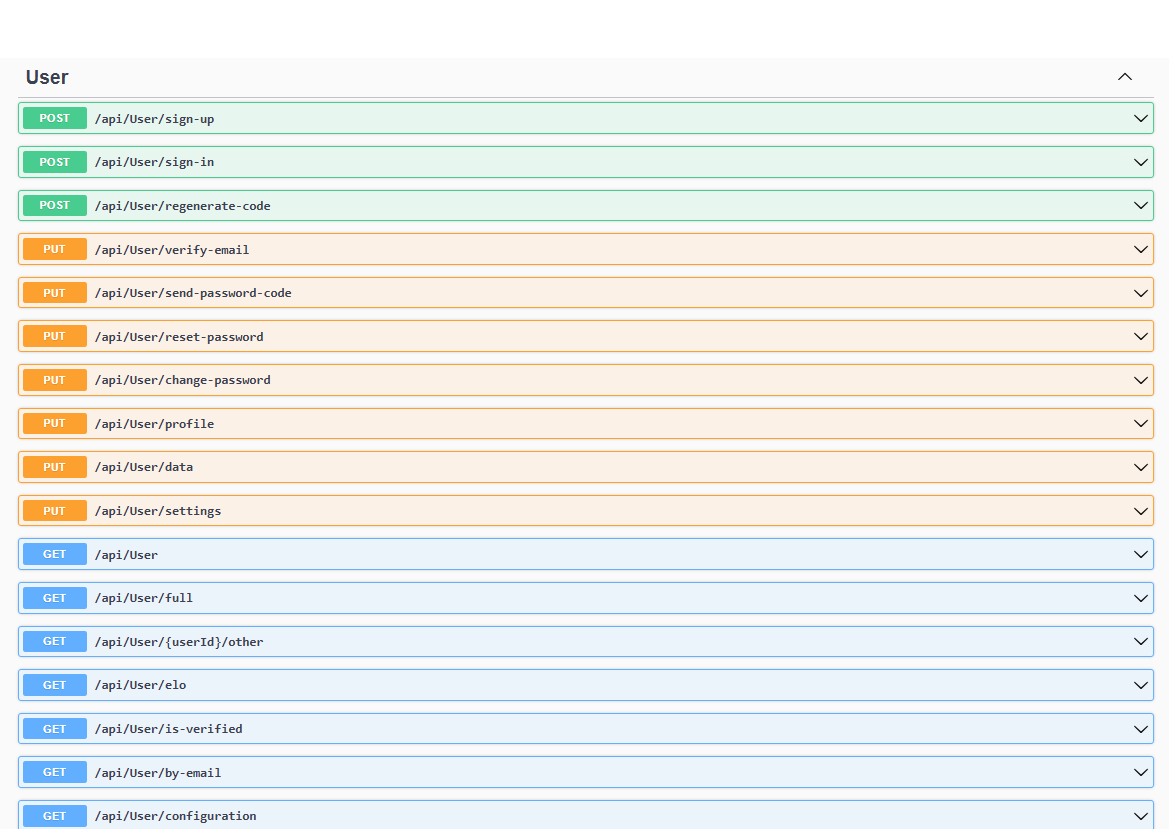
\includegraphics[width=1\textwidth]{zdj/user_controller.png}
        \caption{Punkty końcowe API do rejestracji użytkowników, uwierzytelniania i zarządzania profilami.}
    \end{figure}

    \newpage

    \item \textbf{FriendshipController}
    \begin{itemize} 
        \item \textbf{POST /api/friendship/invite} - Tworzy zaproszenie do znajomości z oczekującym statusem. 
        \item \textbf{POST /api/friendship/block} - Tworzy zaproszenie do znajomości z odrzuconym statusem. 
        \item \textbf{PUT /api/friendship/{friendshipId}/respond} - Zmienia status oczekującej znajomości (akceptacja lub odrzucenie zaproszenia). 
        \item \textbf{GET /api/friendship/all-by-status} - Pobiera wszystkich użytkowników z określonym statusem relacji (np. znajomi, oczekujący). 
        \item \textbf{GET /api/friendship/all-non} - Pobiera wszystkich użytkowników, którzy nie są w relacji z użytkownikiem. 
        \item \textbf{GET /api/friendship/{friendshipId}/profile} - Pobiera profil znajomego na podstawie identyfikatora znajomości. 
        \item \textbf{GET /api/friendship/ranking} - Pobiera ranking użytkowników wśród znajomych na podstawie wybranego modelu. 
        \item \textbf{GET /api/friendship/{friendshipId}/games} - Pobiera listę gier rozegranych w ramach znajomości. 
        \item \textbf{DELETE /api/friendship/{friendshipId}} - Usuwa znajomość i/lub odblokowuje użytkownika. 
    \end{itemize}
    \begin{figure}[h!]
        \centering
        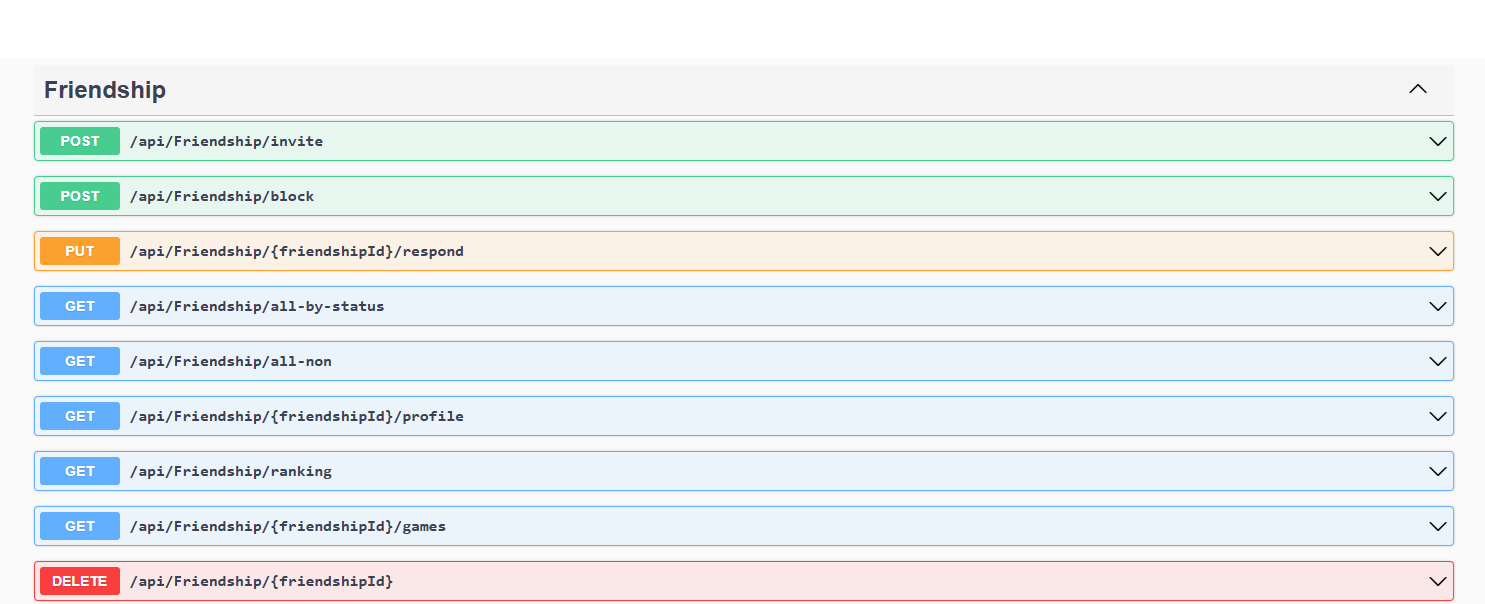
\includegraphics[width=1\textwidth]{zdj/friendship_controller.png}
        \caption{Punkty końcowe API do zarządzania zaproszeniami do znajomych, przyjaźniami i relacjami użytkowników.}
    \end{figure}

    \newpage

    \item \textbf{WebGameController}
    \begin{itemize} 
        \item \textbf{POST /api/webgame/search} - Inicjuje poszukiwanie gry online, tworzy gracza i ustawia czas gry, jeśli nie istnieje. 
        \item \textbf{POST /api/webgame/private} - Tworzy prywatną grę i zwraca jej identyfikator. 
        \item \textbf{POST /api/webgame/email} - Tworzy prywatną grę przez podanie adresu e-mail przeciwnika, zwraca identyfikator gry. 
        \item \textbf{POST /api/webgame/link} - Tworzy prywatną grę z linkiem, który umożliwia dostęp do gry, zwraca identyfikator gry. 
        \item \textbf{GET /api/webgame/is-in-game} - Sprawdza, czy gracz jest już w grze. 
        \item \textbf{GET /api/webgame/{gameId}/update-required} - Sprawdza, czy wymagana jest aktualizacja stanu gry dla gry stworzonej za pomocą linku. 
        \item \textbf{GET /api/webgame/{gameId}} - Pobiera dane jednej gry na podstawie identyfikatora gry. 
        \item \textbf{GET /api/webgame/{gameId}/player} - Pobiera dane gracza w danej grze. 
        \item \textbf{GET /api/webgame/{gameId}/time} - Pobiera czas pozostały dla gracza w danej grze. 
        \item \textbf{GET /api/webgame/{gameId}/opponent} - Pobiera dane przeciwnika z zakończonej gry. 
        \item \textbf{GET /api/webgame/{gameId}/timing} - Pobiera konfigurację czasu gry (timing) dla danej gry. 
        \item \textbf{GET /api/webgame/all-ongoing} - Pobiera wszystkie aktywne gry dla użytkownika. 
        \item \textbf{GET /api/webgame/all-finished} - Pobiera wszystkie zakończone gry dla użytkownika. 
        \item \textbf{GET /api/webgame/type-history} - Pobiera historię gier dla wybranego typu czasu gry. 
        \item \textbf{GET /api/webgame/invitations} - Pobiera wszystkie zaproszenia do gier, które zostały jeszcze nieodebrane. 
        \item \textbf{GET /api/webgame/{gameId}/messages} - Pobiera wszystkie wiadomości z danej gry. 
        \item \textbf{GET /api/webgame/stats} - Pobiera statystyki wszystkich gier rozegranych przez użytkownika. 
        \item \textbf{DELETE /api/webgame/abort} - Anuluje poszukiwanie gry online. 
        \item \textbf{DELETE /api/webgame/{gameId}/cancel} - Anuluje prywatną grę, usuwając graczy. 
    \end{itemize}
    \begin{figure}[h!]
        \centering
        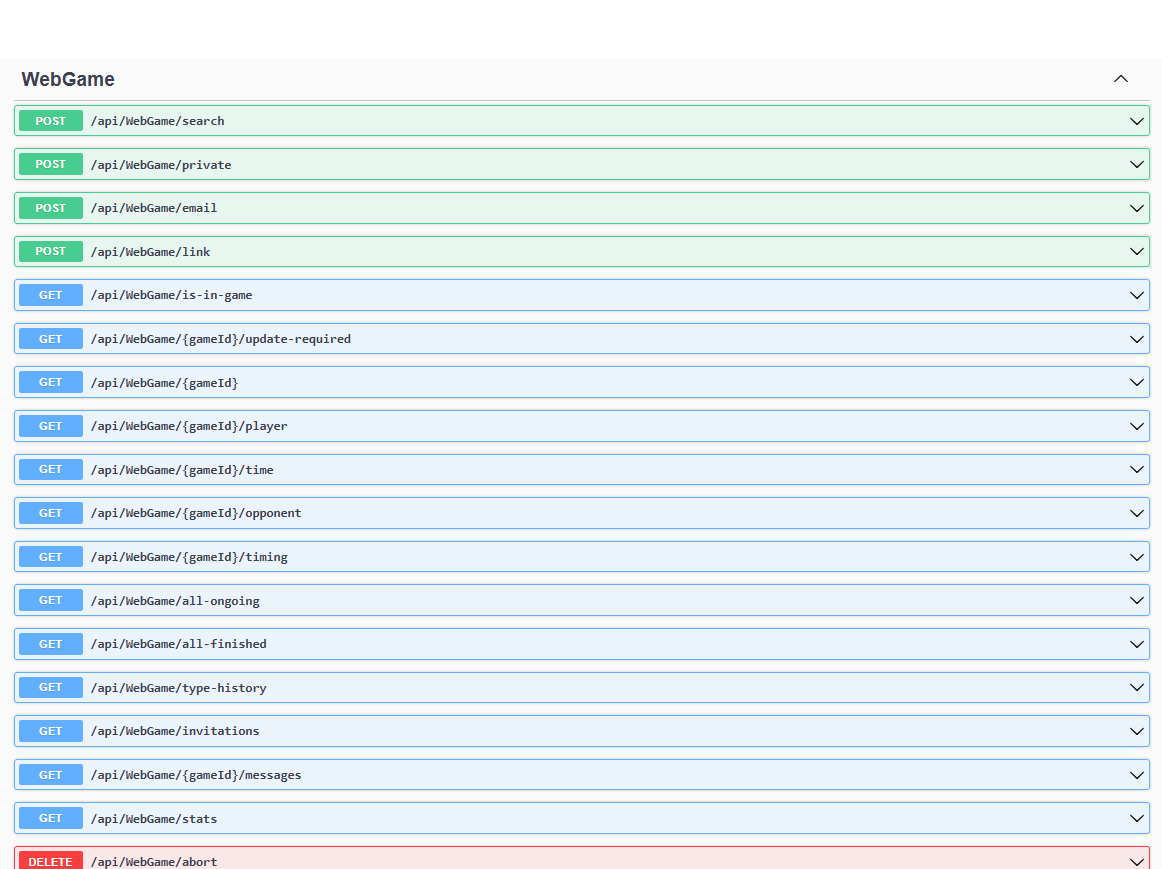
\includegraphics[width=1\textwidth]{zdj/webgame_controller.png}
        \caption{Punkty końcowe API do zarządzania grami sieciowymi, w tym wyszukiwania, tworzenia i sprawdzania statusu graczy w grach publicznych i prywatnych.}
    \end{figure}

    \newpage

    \item \textbf{EngineGameController}
    \begin{itemize} 
        \item \textbf{POST /api/enginegame/start} - Rozpoczyna nową grę z silnikiem szachowym. 
        \item \textbf{POST /api/enginegame/{gameId}/make-move} - Wykonuje ruch w grze, wykonany przez gracza lub silnik.
        \item \textbf{PUT /api/enginegame/{gameId}/end-game} - Kończy grę z silnikiem szachowym. 
        \item \textbf{PUT /api/enginegame/{gameId}/change-engine} - Zmienia poziom trudności silnika szachowego. 
        \item \textbf{PUT /api/enginegame/{gameId}/undo-move} - Cofnięcie ostatniego wykonanego ruchu. 
        \item \textbf{PUT /api/enginegame/update-settings} - Aktualizuje ustawienia związane z grami z silnikiem szachowym. 
        \item \textbf{GET /api/enginegame/{gameId}} - Pobiera wszystkie dane dotyczące gry z silnikiem szachowym.
        \item \textbf{GET /api/enginegame/{gameId}/winner} - Pobiera zwycięzcę gry z silnikiem szachowym. 
        \item \textbf{GET /api/enginegame/{gameId}/engine-move} - Pobiera ruch wykonany przez silnik w grze. 
        \item \textbf{GET /api/enginegame/{gameId}/all-messages} - Pobiera wszystkie wiadomości związane z aktualną grą z silnikiem. 
        \item \textbf{GET /api/enginegame/all-games} - Pobiera wszystkie gry z silnikiem szachowym. 
    \end{itemize}
    \begin{figure}[h!]
        \centering
        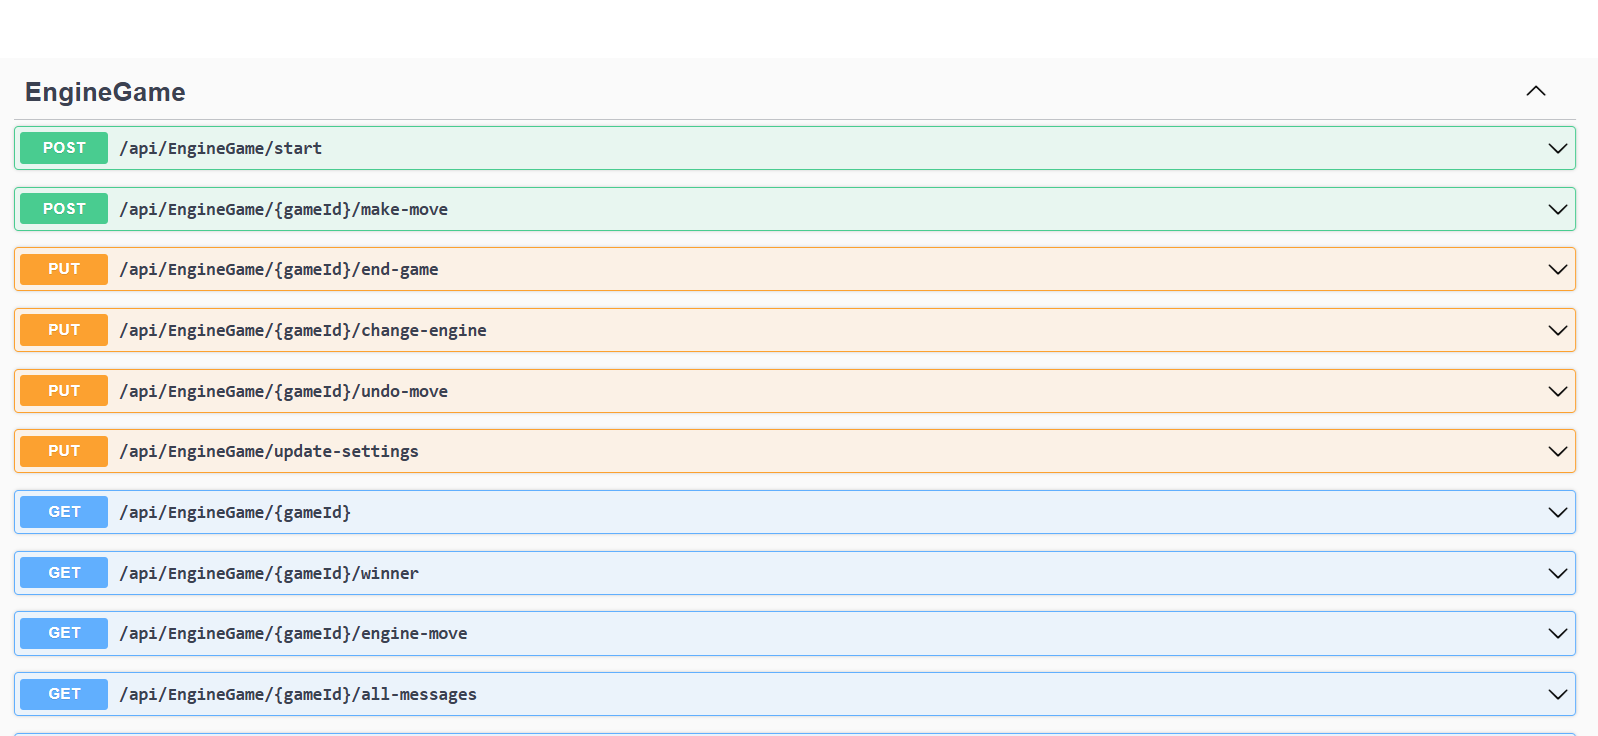
\includegraphics[width=1\textwidth]{zdj/enginegame_controller.png}
        \caption{Punkty końcowe API do zarządzania grami silnika, w tym uruchamiania, wykonywania ruchów, zmiany ustawień i przeglądania danych gry.}
    \end{figure}
\end{itemize}

\newpage
\subsubsection{SignalR}

\newpage
\subsubsection{Komunikacja z silnikiem}
Komunikacja z silnikiem szachowym jest kluczowym elementem w budowie aplikacji, która ma na celu interakcję z popularnymi silnikami szachowymi, takimi jak Stockfish. W przedstawionym przykładzie wykorzystano klasę EngineService, która zapewnia funkcjonalność umożliwiającą komunikację z procesem silnika.

Klasa EngineService implementuje interfejs IEngineService, co zapewnia jednolitość i ułatwia integrację z innymi komponentami aplikacji. W konstruktorze tej klasy tworzony jest obiekt typu Process, który uruchamia silnik szachowy. Proces jest konfigurowany tak, aby nie tworzył okna i umożliwiał przesyłanie danych zarówno do silnika - poprzez standardowe wejście, jak i z silnika - poprzez standardowe wyjście.

\begin{itemize} 
    \item \textbf{Startowanie procesu silnika:} W konstruktorze klasy, obiekt typu Process jest konfigurowany za pomocą klasy ProcessStartInfo. Ustawienia te zapewniają, że silnik będzie działał w tle bez interakcji z interfejsem użytkownika, a komunikacja będzie odbywała się za pomocą strumieni wejścia i wyjścia. 
    \item \textbf{Wysyłanie komend do silnika:} Metoda SendCommand pozwala na wysyłanie komend do silnika. Komendy są przesyłane do standardowego wejścia silnika, a następnie natychmiastowo zapisywane do strumienia wyjściowego. 
    \item \textbf{Odczytywanie wyników:} Metoda ReadOutput służy do odczytywania danych wyjściowych z silnika. Wykorzystuje ona strumień wyjściowy, by zbierać linie tekstu, które są następnie przechowywane w liście. Proces odczytu jest ograniczony czasowo, co zapobiega zablokowaniu aplikacji w przypadku długotrwałych odpowiedzi silnika. 
    \item \textbf{Zamykanie procesu:} Metoda Close wysyła do silnika komendę quit, a następnie zamyka proces, kończąc w ten sposób interakcję z silnikiem. 
\end{itemize}

Dzięki takiej implementacji, aplikacja może komunikować się z silnikiem szachowym w sposób asynchroniczny i kontrolować przebieg gry w czasie rzeczywistym, co jest fundamentem wielu aplikacji szachowych.

\newpage
\subsubsection{Mechanizmy gry i zarządzanie stanem}

\textbf{Tworzenie i dołączanie do gier}\\
Proces tworzenia i dołączania do gier w aplikacji można podzielić na trzy główne typy: gry online z losowym graczem, prywatne gry online oraz gry z komputerem (silnikiem). Każdy z tych typów ma swoją specyficzną logikę, która determinuje sposób, w jaki gracze dołączają do gier oraz jak te gry są inicjowane.

\begin{itemize}
    \item \textbf{Gry online z losowym graczem}\\
    W przypadku gier online z losowym graczem, użytkownik rozpoczyna proces poszukiwania gry, co skutkuje utworzeniem tzw. "gracza". Gracz ten trafia do kolejki oczekujących, gdzie oczekuje na innych graczy. Każde dołączenie nowego gracza do tej samej kolejki wywołuje mechanizm, który zbiera wszystkich oczekujących graczy i sprawdza, czy warunki do rozpoczęcia gry zostały spełnione.
    \\
    Sprawdzanie, czy można rozpocząć grę, odbywa się w sposób sekwencyjny, zaczynając od graczy, którzy oczekują najdłużej. Jeżeli warunki (np. odpowiednia liczba graczy, odpowiednia punktacja lub poziom doświadczenia) zostaną spełnione, gra zostaje utworzona. Wówczas gracz i jego przeciwnik, wybrany na podstawie zbliżonej punktacji, są automatycznie dodawani do gry, rozpoczynając wspólną rozgrywkę.
    
    \item \textbf{Prywatne gry online}\\
    Prywatne gry online różnią się od gier losowych tym, że są one tworzone automatycznie przez graczy, którzy posiadają zaproszenie do wspólnej gry. W tym przypadku gra jest tworzona z góry, a gracze zostają od razu przypisani do tej gry, nie oczekując w kolejce.
    \\
    Prywatne gry mają specyficzną cechę — gracze biorący udział w takich grach są oznaczani jako "prywatni". Tacy gracze nie są uwzględniani w systemie wyszukiwania gier online, co oznacza, że nie mogą brać udziału w losowych dobieraniach graczy (zgodnie z opisanym wcześniej mechanizmem dla gier online). W związku z tym, prywatne gry odbywają się wyłącznie pomiędzy zaproszonymi graczami.

    \item \textbf{Gry z komputerem}\\
    W przypadku gier z komputerem, proces jest najbardziej zautomatyzowany. Gra z komputerem jest tworzona automatycznie, a użytkownik jest jedynym graczem w grze. Gra nie wymaga oczekiwania na innych graczy, ponieważ przeciwnikiem użytkownika jest komputer. W tym przypadku tworzony jest tylko jeden gracz reprezentujący użytkownika, który bierze udział w grze przeciwko sztucznej inteligencji (silnikowi).
\end{itemize}

\textbf{Powiadomienia o zmianach stanu kolejki}\\
Aby zapewnić synchronizację pomiędzy graczami i ich reakcję na zmiany stanu kolejki, aplikacja wykorzystuje technologię SignalR. Jest to narzędzie, które pozwala na natychmiastową synchronizację stanu gry pomiędzy graczami, zapewniając, że każdy gracz jest na bieżąco informowany o tym, czy został dołączony do gry, lub czy otrzymał zaproszenie do prywatnej gry. Dzięki SignalR gracze mogą otrzymywać powiadomienia w czasie rzeczywistym, co umożliwia im płynne przejście do etapu gry bez opóźnień.

\newpage
\textbf{Punktacja ELO}\\
Punktacja ELO to system oceny umiejętności graczy stosowany w aplikacji do określania ich relatywnej siły gry. Mechanizm ten jest dynamiczny, co oznacza, że po każdej zakończonej grze punkty ELO obu graczy są aktualizowane w zależności od wyniku rozgrywki. Wartość zmiany w punktacji jest obliczana na podstawie różnicy punktów między graczami oraz wyniku gry. System ELO uwzględnia pięć kategorii czasowych rozgrywek: bullet, blitz, rapid, classic oraz daily, z których każda ma osobną punktację. Do obliczenie punktacji rozróżnia się trzy główne przypadki:

\begin{itemize}
    \item \textbf{Wygrana lepszego gracza}\\
    Jeśli zwycięzcą gry jest gracz, który przed rozgrywką miał wyższą punktację ELO niż jego przeciwnik, oznacza to, że wynik był bardziej przewidywalny. W takim przypadku zmiana punktacji dla zwycięzcy oraz przegranego jest stosunkowo niewielka, ponieważ potwierdza ona wcześniejsze przypuszczenia o różnicy w umiejętnościach graczy.

    \[ \text{elo}_{\pm} = \lceil \frac{100}{0.1 \cdot \Delta \text{elo} + 10} \rceil \]

    Gdzie $ \text{elo}_{\pm} $ oznacza punkty dodane / odjęte graczom a $ \Delta \text{elo} $ oznacza różnice w punktacji pomiędzy graczami przez rozpoczęciem gry.\\

    Im większa różnica w punktacji ELO między graczami, tym mniejsza zmiana punktów dla zwycięzcy, co odzwierciedla mniejsze znaczenie wygranej dla wyżej punktowanego gracza.
    \item \textbf{Wygrana słabszego gracza}\\
    Jeśli zwycięzcą gry jest gracz z niższą punktacją ELO niż jego przeciwnik, wynik jest bardziej zaskakujący, co prowadzi do większych zmian punktacji. W takim przypadku stosuje się wzór:

    \[ \text{elo}_{\pm} = \lceil 0.1 \cdot \Delta \text{elo} + 10 \rceil \]

    Gdzie $ \text{elo}_{\pm} $ oznacza punkty dodane / odjęte graczom a $ \Delta \text{elo} $ oznacza różnice w punktacji pomiędzy graczami przez rozpoczęciem gry.\\

    W tym przypadku, większa różnica punktów ELO działa na korzyść zwycięzcy, co skutkuje znaczącym wzrostem jego punktacji. Analogicznie, przegrany, który był wyżej punktowany, traci więcej punktów, co odzwierciedla większą wagę niespodziewanego wyniku.

    \item \textbf{Przypadek remisu}\\
    Remis jest traktowany jako sytuacja, w której obaj gracze osiągają równy wynik, co skutkuje mniejszą zmianą punktacji niż w przypadku zwycięstwa jednego z graczy. Zmiana punktacji w przypadku remisu zależy również od różnicy punktów między graczami. Stosowany jest wzór:

    \[ \text{elo}_{\pm} = \lceil 0.05 \cdot \Delta \text{elo} \rceil \]

    Gdzie $ \text{elo}_{\pm} $ oznacza punkty dodane / odjęte graczom a $ \Delta \text{elo} $ oznacza różnice w punktacji pomiędzy graczami przez rozpoczęciem gry.\\

    \newpage
    W tym przypadku:
    \begin{itemize}
        \item Gracz z wyższą punktacją ELO traci punkty, ponieważ wynik jest mniej korzystny dla jego reputacji jako silniejszego gracza.
        \item Gracz z niższą punktacją ELO zyskuje punkty, ponieważ remis z bardziej doświadczonym przeciwnikiem jest dla niego korzystnym rezultatem.
    \end{itemize}
\end{itemize}

Poniższy wykres ilustruje zależność zmiany punktacji ELO, gdzie $ \text{y} = \text{elo}_{\pm} $ od różnicy punktacji między graczami $ \text{x} = \Delta \text{elo} $  w trzech wyżej wymienionych scenariuszach. Każda z tych sytuacji jest modelowana za pomocą odpowiedniej funkcji, co pozwala zobaczyć, jak zmieniają się wartości punktów dodawanych lub odejmowanych w zależności od poziomu graczy.

\begin{figure}[h!]
    \centering
    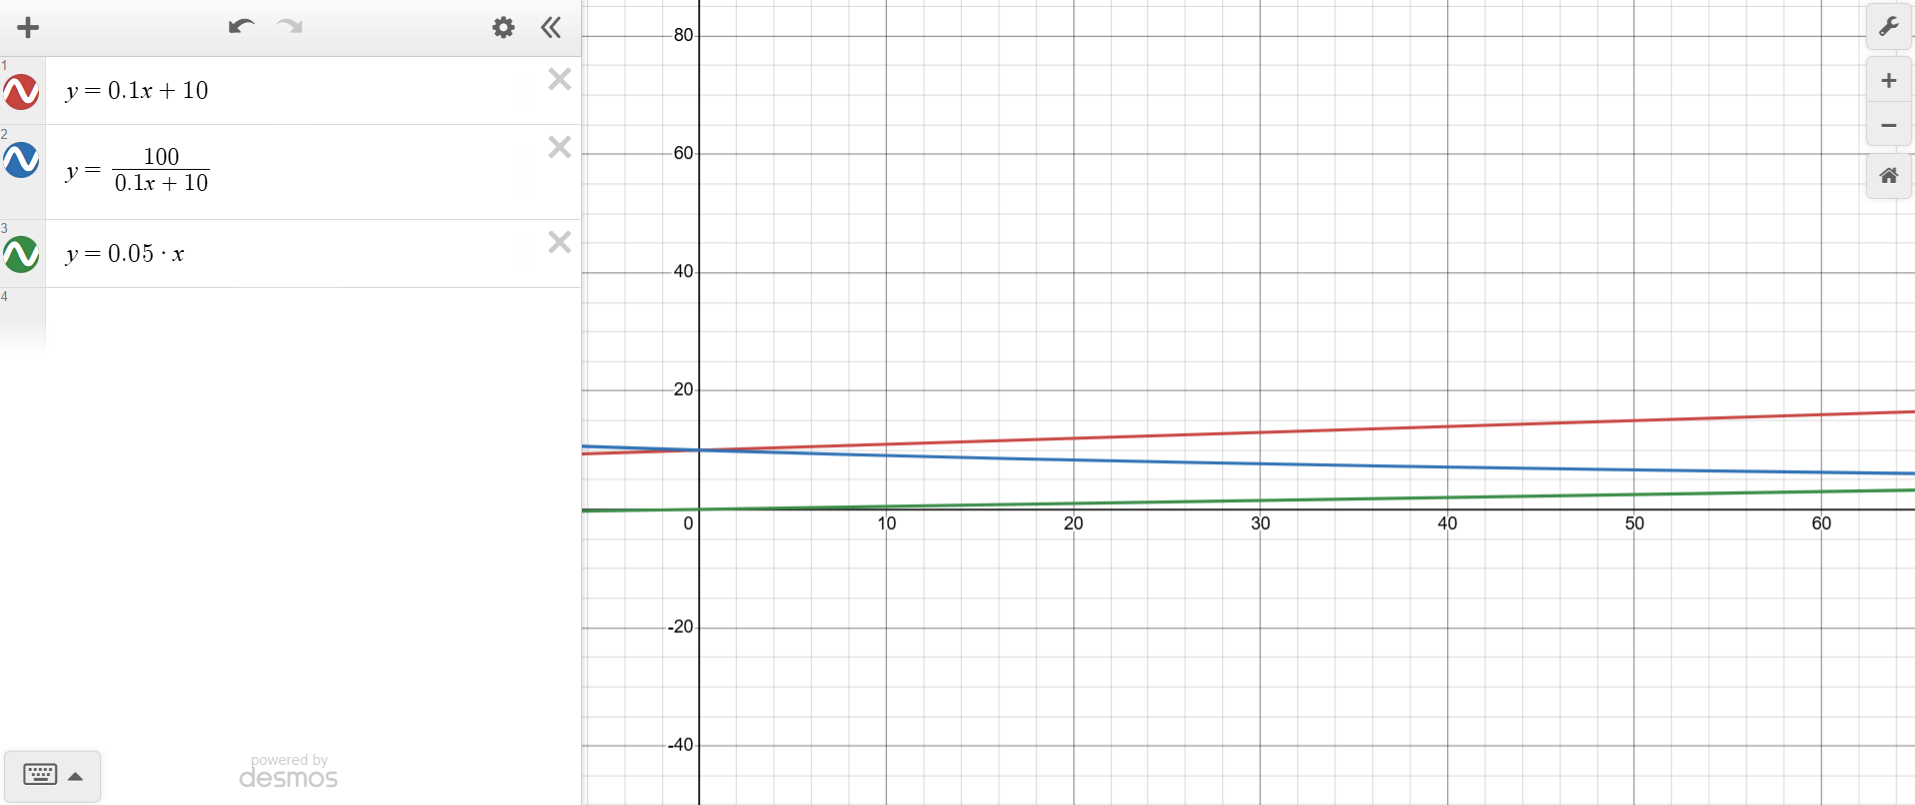
\includegraphics[width=1\textwidth]{zdj/elo_calc.png}
    \caption{Zmiana punktacji ELO w zależności od różnicy poziomu graczy - wykresy utworzone za pomocą strony www.desmos.com}
\end{figure}

System ELO w aplikacji jest zoptymalizowany, aby sprawiedliwie odzwierciedlać wyniki rozgrywek. Wzory uwzględniają różnicę umiejętności między graczami, nagradzając trudniejsze zwycięstwa i minimalizując znaczenie wyników oczekiwanych. Dzięki tym zasadom system punktacji motywuje graczy do rozwoju i rywalizacji, zachowując jednocześnie równowagę w ocenie ich umiejętności.
\\\\

\textbf{Punktacja gry z silnikiem}\\
Punktacja ELO w przypadku gier z silnikiem różni się od tej stosowanej w grach między graczami. Ma ona charakter symboliczny i informacyjny, a jej celem jest głównie odzwierciedlenie wyniku starcia z komputerowym przeciwnikiem. Wyniki z gier z silnikiem nie są uwzględniane w oficjalnych rankingach aplikacji. Mechanizm ten działa w następujący sposób: w zależności od poziomu silnika (od 1 do 20), punktacja jest modyfikowana odpowiednio do wyniku gry. Jeśli gracz przegra z silnikiem, od jego ELO jest odejmowany poziom silnika, natomiast jeśli gracz wygra, do jego ELO jest dodawany poziom silnika. Dzięki temu użytkownicy mogą w przybliżeniu ocenić swoje umiejętności względem różnych poziomów trudności silnika, co może stanowić dla nich dodatkową motywację i wskaźnik postępu.

\newpage
\textbf{Zarządzanie czasem gry}\\
W szachach istnieje kilka różnych typów ustawienia czasu, które mają wpływ na dynamikę gry. W zależności od wybranego typu, gracze mają różne limity czasowe na wykonanie swoich ruchów. Każdy z tych typów jest dostosowany do innego tempa rozgrywki, co pozwala na dopasowanie doświadczenia gry do preferencji graczy. Czas gry w szachach może obejmować różne długości, poczynając od błyskawicznych partii typu "Bullet", po długoterminowe gry "Daily", gdzie gracze wykonują ruchy w ciągu wielu dni.
\\\\
Poniżej przedstawiona jest tabela pokazująca różne typy czasów gry w szachach:

\begin{table}[h!]
    \centering
    \begin{tabular}{|l|m{3cm}|m{3cm}|m{5cm}|}
        \hline
        \textbf{Typ Czasu} & \textbf{Zakres Czasu} & \textbf{Inkrement} & \textbf{Charakterystyka} \\ \hline
        \textbf{Bullet} & 1 - 3 minut & 0 - 60 sek. & Bardzo szybka gra. \\ \hline
        \textbf{Blitz} & 3 - 10 minut & 0 - 60 sek. & Gra o szybkim tempie. \\ \hline
        \textbf{Rapid} & 10 - 60 minut & 0 - 60 sek. & Gra o średnim tempie. \\ \hline
        \textbf{Classic} & 60 - 1440 minut & 0 - 60 sek. & Dużą ilością czasu. \\ \hline
        \textbf{Daily} & $\geq$ 1440 minut & 0 - 60 sek. & Bardzo długi czas gry. \\ \hline
    \end{tabular}
    \caption{Rodzaje czasów gry w szachach}
\end{table}


Podczas pierwszego pobrania gry przez graczy ustalany jest czas rozpoczęcia partii. Następnie, przy każdym wykonanym ruchu, system oblicza, ile czasu minęło od ostatniego zarejestrowanego momentu (czy to od rozpoczęcia gry, czy od ostatniego ruchu). Na podstawie tej różnicy czasu, system aktualizuje pozostały czas dla gracza, odejmując upływający czas od jego pozostałego limitu. Dodatkowo, po każdym ruchu do czasu pozostałego dla gracza dodawany jest inkrement (czas przyznawany za wykonanie ruchu). Czas jest aktualizowany osobno dla każdego z graczy, w zależności od tego, która tura jest aktualnie wykonywana.
\\\\
Aplikacja posiada także zaimplementowane zadanie cykliczne, które jest uruchamiane co minutę, aby monitorować postęp czasu w długoterminowych trybach gry, takich jak "Classic" i "Daily", ale także do pozostałych trybów (np: w przypadkach opuszczenia strony przez użytkownika). Zadanie to sprawdza, czy któremuś z graczy nie skończył się czas, co mogłoby skutkować zakończeniem gry. System analizuje, kiedy ostatni ruch został zarejestrowany i oblicza różnicę między tym czasem a bieżącym czasem. Na tej podstawie, dla każdego gracza obliczany jest pozostały czas, a jeżeli czas gracza którego jest tura upłynie, system uznaje go za przegranego. Jeśli jeden z graczy przekroczy swój limit czasowy, gra jest automatycznie kończona.

\begin{figure}[h!]
    \centering
    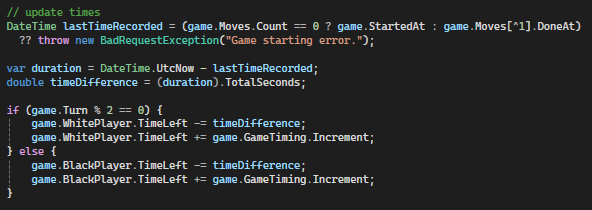
\includegraphics[width=1\textwidth]{zdj/update_times.png}
    \caption{Fragment kodu przedstawiający aktualizacje czasu graczy.}
\end{figure}

\newpage
\subsubsection{Pozostałe kluczowe aspekty}

\textbf{Przetwarzanie zapytań}\\
W systemie przetwarzania zapytań wykorzystywana jest biblioteka MediatR, która umożliwia zarządzanie zapytaniami w sposób przejrzysty i modularny. MediatR opiera się na wzorcu projektowym Mediator, co pozwala na oddzielenie logiki przetwarzania zapytań od innych komponentów aplikacji.
\\\\
W tym systemie każde zapytanie, na przykład żądanie wykonania jakiejś operacji, pobrania danych lub zapisania ich, jest reprezentowane przez obiekt, który dziedziczy po interfejsie IRequest<T>, gdzie T oznacza typ odpowiedzi, którą zapytanie zwróci. Zapytania te są przekazywane do mediatorów, którzy następnie kierują je do odpowiednich handlerów, czyli klas odpowiedzialnych za wykonanie logiki związanej z zapytaniem.
\\\\

\textbf{Przebieg przetwarzania zapytania}
\begin{enumerate}
    \item \textbf{Zgłoszenie zapytania:} Kiedy klient wyśle zapytanie do systemu przez API lub SignalR, zapytanie to jest mapowane na odpowiedni Request, który może zawierać dane wejściowe potrzebne do przetworzenia.
    \item \textbf{Przetwarzanie zapytania:} Zapytanie trafia do MediatR, który przekazuje je do odpowiedniego handlera. Handler jest odpowiedzialny za wykonanie logiki biznesowej.
    \item \textbf{Wykonanie akcji:} Handler wykonuje określoną akcję. Może to być np. zapis do bazy danych, obliczenie wyniku gry, aktualizacja punktacji ELO lub inne działania biznesowe.
    \item \textbf{Zwrócenie odpowiedzi:} Po wykonaniu akcji, handler zwraca odpowiedź (np. dane w formie obiektu, kod statusu, wynik operacji). MediatR przekazuje tę odpowiedź z powrotem do klienta.
\end{enumerate}

W systemie, który obsługuje zapytania, każde zapytanie jest reprezentowane przez osobny obiekt zapytania, który jest mapowany na Request. Każdy Request posiada przypisany handler, który odpowiedzialny jest za realizację zapytania.
\\\\

\textbf{Zalety wykorzystania MediatR:}
\begin{itemize}
    \item \textbf{Separation of Concerns:} MediatR pozwala na oddzielenie logiki przetwarzania zapytań od innych części aplikacji, takich jak kontrolery czy warstwa interfejsu użytkownika.
    \item \textbf{Skalowalność i modularność:} Dzięki wykorzystaniu handlerów, system jest łatwiejszy do rozszerzania i utrzymania. Każda operacja jest odseparowana w osobnym komponencie, co ułatwia zarządzanie kodem.
    \item \textbf{Testowalność:} Każdy handler można testować niezależnie, co ułatwia implementację testów jednostkowych.
    \item \textbf{Centralizacja logiki:} Logika biznesowa jest centralizowana w handlerach, co zapewnia spójność i łatwość w zarządzaniu.
\end{itemize}

\newpage
\textbf{Rezultaty zapytań i paginacja}\\
W systemie, zwracane są także odpowiedzi, które mogą zawierać dane w różnych formach. W przypadku wielu zapytań, szczególnie tych związanych z wyszukiwaniem lub pobieraniem dużej ilości danych, wykorzystuje się specjalne klasy, które umożliwiają mapowanie wyników na odpowiednie modele. Część zapytań zwraca dane w postaci DTO (Data Transfer Object), które są prostymi obiektami przechowującymi dane. Te obiekty są mapowane z encji bazy danych, co pozwala na łatwiejsze i bardziej kontrolowane przekazywanie danych pomiędzy warstwami aplikacji.
\\\\
W przypadku, gdy zapytanie dotyczy wielu elementów (np. listy gier), zastosowana jest paginacja – technika, która pozwala na dzielenie dużych zbiorów danych na mniejsze części (strony), co znacznie poprawia wydajność i doświadczenie użytkownika, ograniczając ilość danych przesyłanych w jednym żądaniu. Dzięki paginacji zamiast zwracać wszystkie dane na raz, system zwraca tylko określoną liczbę elementów na stronie oraz informację o numerze strony. Dzięki temu, gdy liczba elementów jest duża, użytkownik może nawigować po wynikach w sposób bardziej wydajny, ładować tylko potrzebne dane i nie obciążać systemu nadmiernym przesyłaniem informacji.
\\\\
Aby wspierać paginację, w systemie zostały zaimplementowane dwie klasy:
\begin{itemize}
    \item \textbf{PagedRequest:} Ogólna klasa, z której dziedziczą modele i zapytania wymagające paginacji. Zawiera parametry określające numer strony oraz rozmiar strony, które są używane do obliczenia, które elementy mają zostać zwrócone.
    \item \textbf{PagedResult<T>:} Klasa, która jest używana do zwracania wyników zapytania z paginacją. Przyjmuje generyczny typ T, który odpowiada za dane zwracane w odpowiedzi, takie jak DTO. Klasa ta zawiera szczegóły dotyczące wyników: listę elementów, łączną liczbę stron, numerację wyników oraz całkowitą liczbę elementów.
\end{itemize}

\begin{figure}[h!]
    \centering
    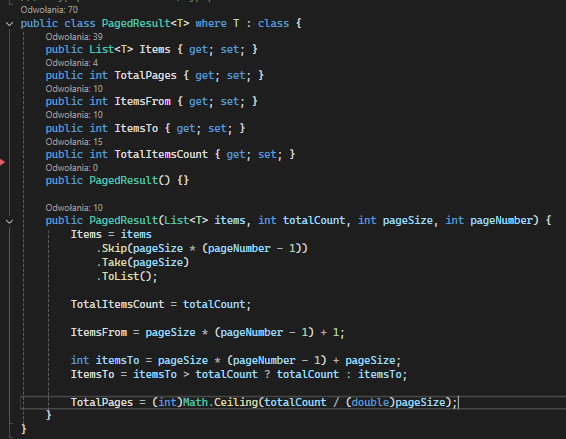
\includegraphics[width=0.7\textwidth]{zdj/pagination.png}
    \caption{Klasa rezultatu paginacji.}
\end{figure}

\newpage
\textbf{Serwis SMTP}\\
Serwis SMTP (Simple Mail Transfer Protocol) jest wykorzystywany w aplikacji do obsługi wysyłania wiadomości e-mail, co obejmuje zarówno proces weryfikacji e-maila użytkowników, jak i powiadamianie o zaproszeniach do gry. W aplikacji implementacja serwisu SMTP umożliwia automatyczne generowanie i wysyłanie e-maili w różnych scenariuszach, takich jak potwierdzenie rejestracji, resetowanie hasła, czy zaproszenia do gier.
\\\\
Serwis SMTP, za pomocą klasy SmtpService, korzysta z biblioteki .NET, która umożliwia konfigurację połączeń z serwerem pocztowym i wysyłanie e-maili. Serwis ten jest skonfigurowany przy użyciu opcji zawartych w appsettings.json, który przechowuje dane potrzebne do połączenia z serwerem SMTP (adres hosta, port, dane logowania, itp.).
\\\\
Serwis implementuje kilka kluczowych metod umożliwiających wysyłkę maili, służących do weryfikacji lub otrzymywania powiadomień. Wszystkie metody w serwisie tworzą wiadomość e-mail, której treść jest zbudowana w formacie HTML, co umożliwia bardziej zaawansowane formatowanie, w tym wstawianie obrazków, linków czy kodów.
\\\\
Wszystkie e-maile są wysyłane przez SmtpClient, który łączy się z odpowiednim serwerem SMTP (na podstawie danych konfiguracyjnych) i wysyła wiadomość do wskazanego odbiorcy. Dzięki asynchroniczności operacji, wysyłanie e-maili nie blokuje głównego wątku aplikacji, co zapewnia płynność działania systemu.
\\\\

\textbf{Serwis JWT}\\
Serwis JWT (JSON Web Token) w aplikacji służy do generowania tokenów autoryzacyjnych, które są wykorzystywane do uwierzytelniania użytkowników oraz zapewnienia dostępu do chronionych zasobów aplikacji. Tokeny JWT są powszechnie stosowane w aplikacjach webowych do obsługi logowania i autoryzacji, a ich głównym celem jest umożliwienie użytkownikowi dostępu do określonych zasobów, bez konieczności ponownego wprowadzania danych logowania przy każdym żądaniu.
\\\\
Implementacja serwisu JWT w aplikacji opiera się na klasie, która zawiera metodę GetJwtToken. Metoda ta przyjmuje obiekt User, który reprezentuje zalogowanego użytkownika, a na podstawie jego danych generuje unikalny token. Serwis ten generuje tokeny uwierzytelniające użytkowników. Na początku tworzy zestaw roszczeń, takich jak identyfikator, nazwa użytkownika, rola i status weryfikacji e-maila. Token jest podpisywany za pomocą klucza przechowywanego w ustawieniach aplikacji, używając algorytmu HMAC-SHA256. Określana jest również data wygaśnięcia tokenu, np. po 7 dniach. Następnie tworzony jest obiekt JwtSecurityToken, który zawiera claims, datę wygaśnięcia i podpisane dane. Token jest serializowany do formatu string i przesyłany w odpowiedzi do klienta.
\\\\
Serwis JWT stanowi kluczowy element systemu autoryzacji w aplikacji, umożliwiając bezpieczne zarządzanie dostępem do chronionych zasobów w systemie. Użytkownicy, którzy zalogują się do aplikacji, otrzymują token JWT, który musi być dołączony do każdego żądania do API, aby potwierdzić tożsamość i autoryzację.

\newpage
\textbf{Entity Framework}\\

\newpage
\subsubsection{Wykorzystane pakiety i biblioteki}

W projekcie zastosowano szereg bibliotek, które wspierają rozwój i funkcjonalność aplikacji. Każda z wymienionych bibliotek została dobrana w celu spełnienia konkretnych wymagań funkcjonalnych i architektonicznych projektu, co pozwala na jego rozwój zgodny z najlepszymi praktykami. Poniżej przedstawiono szczegółowy opis wybranych komponentów:
\begin{itemize} 
    \item \textbf{Swashbuckle.AspNetCore} i \textbf{SignalRSwaggerGen}: Obie biblioteki służą do generowania dokumentacji Swagger, co pozwala na dokumentowanie API REST i SignalR w jednej konfiguracji. 
    \item \textbf{AutoMapper}: Biblioteka umożliwiająca mapowanie obiektów między różnymi warstwami aplikacji, eliminując potrzebę ręcznego mapowania. 
    \item \textbf{MediatR}: Implementuje wzorzec Mediatora, co umożliwia luźne powiązanie komponentów aplikacji i jest powszechnie wykorzystywane w aplikacjach opartych na wzorcu CQRS. 
    \item \textbf{Npgsql.EntityFrameworkCore.PostgreSQL} i \textbf{Microsoft.EntityFrameworkCore}: Npgsql to dostawca dla Entity Framework Core dla bazy danych PostgreSQL, co umożliwia korzystanie z tej bazy danych za pomocą EF Core w aplikacjach .NET. 
    \item \textbf{FluentAssertions}: Biblioteka do tworzenia bardziej czytelnych i wyrażających zamiar asercji w testach jednostkowych. 
    \item \textbf{Microsoft.AspNetCore.SignalR} i \textbf{Microsoft.AspNetCore.Cors}: Obie biblioteki obsługują komunikację w czasie rzeczywistym oraz kontrolują dostęp do zasobów serwera z innych domen w aplikacjach webowych. 
    \item \textbf{Microsoft.AspNetCore.Identity} i \textbf{Microsoft.AspNetCore.Authentication.JwtBearer}: Biblioteki związane z bezpieczeństwem aplikacji, wspierające mechanizmy uwierzytelniania i autoryzacji, w tym logowanie z użyciem JWT. 
    \item \textbf{Microsoft.AspNetCore.Mvc.Core} i \textbf{Microsoft.AspNetCore.Mvc.Testing}: Obie biblioteki są odpowiedzialne za budowanie endpointów API oraz testowanie aplikacji, w tym kontrolerów i routingu. 
    \item \textbf{Microsoft.IdentityModel.Tokens}: Biblioteka do obsługi tokenów, takich jak JWT, niezbędna do tworzenia i weryfikacji tokenów w aplikacjach z uwierzytelnianiem opartym na tokenach. 
    \item \textbf{Microsoft.Extensions.*}: Zestaw bibliotek wspierających konfigurację aplikacji oraz wstrzykiwanie zależności, kluczowy dla budowy skalowalnych aplikacji.
    \item \textbf{Microsoft.NET.Test.Sdk}, \textbf{xUnit}, \textbf{xUnit.runner.visualstudio} i \textbf{Moq}: Zestaw bibliotek do testowania aplikacji, wspierający tworzenie testów jednostkowych i integracyjnych, w tym generowanie mocków i uruchamianie testów w Visual Studio. 
\end{itemize}

\newpage
\subsection{Frontend}
\subsubsection{Architektura}

Struktura frontendu w tym projekcie jest zorganizowana w sposób umożliwiający łatwe zarządzanie kodem, dzięki zastosowaniu odpowiednich folderów i podfolderów, które odpowiadają za różne aspekty aplikacji. W głównym folderze src znajdują się trzy foldery: index, main oraz shared. Każdy z nich ma swoją specyficzną rolę w organizacji kodu.
\\\\
Folder index zawiera router odpowiedzialny za strony ogólnodostępne, takie jak strona główna, rejestracja czy informacje o aplikacji. Folder main jest przeznaczony do zarządzania zasobami dostępnymi tylko dla zalogowanych i zweryfikowanych użytkowników. Dostęp do tych stron jest kontrolowany na podstawie stanu autoryzacji użytkownika, co zapewnia bezpieczeństwo aplikacji. Folder shared natomiast zawiera komponenty i funkcjonalności, które są współdzielone pomiędzy różnymi częściami aplikacji.

\begin{figure}[h!]
    \centering
    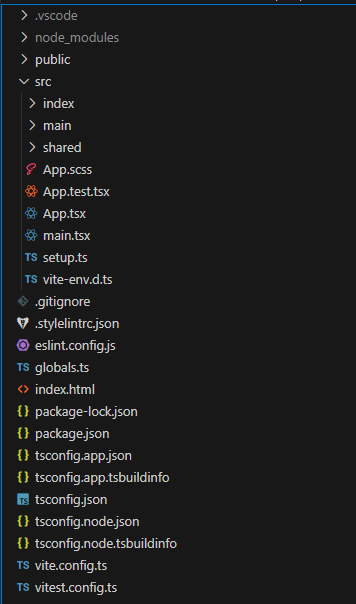
\includegraphics[width=0.5\textwidth]{zdj/struktura_front.png}
    \caption{Struktura projektu.}
\end{figure}


Taka organizacja pozwala na modularność i łatwiejsze utrzymanie aplikacji. Każda z sekcji ma wyraźnie określoną rolę i zakres odpowiedzialności, co sprzyja porządkowi w projekcie i ułatwia pracę.

\newpage
Folder shared w projekcie jest zaprojektowany w sposób, który sprzyja ponownemu wykorzystaniu kodu i organizacji wspólnych zasobów używanych w całej aplikacji. Zawiera on różnorodne podfoldery, które grupują funkcje, komponenty i style, w zależności od ich roli w projekcie.

\begin{itemize}
    \item \textbf{components:} przechowuje małe, wielokrotnie używane komponenty, które są wykorzystywane w różnych miejscach aplikacji. Mogą to być takie elementy jak  przyciski, okna ładowania czy inne fragmenty UI, które są stosowane w różnych częściach aplikacji.
    \item \textbf{styles:} zawiera globalne definicje stylów SCSS. Są tam zdefiniowane zmienne, które ułatwiają zarządzanie kolorami, czcionkami, a także mixiny, które pomagają w definiowaniu jednolitych stylów elementów. Dzięki temu stylowanie jest bardziej spójne i łatwiejsze do modyfikacji w jednym miejscu. Wszystkie współdzielone style są zbierane z różnych plików do jednego - shared.scss, ktory to następnie jest importowany do wszystkich komponentów strony aby umożliwić ich działanie.
    \item \textbf{svgs:} gromadzi wszystkie ikony i mapy ikon, które są wielokrotnie używane w aplikacji. Mapy ikon to funkcje, które na podstawie podanej nazwy ikony zwracają odpowiedni tag svg, co pozwala na łatwe zarządzanie ikonami w projekcie. Do tworzenia ikon stosowany jest specjalny komponent, ktory wymaga podania wybranej mapy oraz nazwy ikon, ktory nastepnie na podstawie tych parametrow zwraca i tworzy odpowiednia ikone.
    \item \textbf{utils:} zawiera dodatkowe narzędzia, które wspomagają działanie aplikacji. Jest podzielony na kilka podfolderów:
    \begin{itemize}
        \item \textbf{functions:} zawiera globalne i współdzielone funkcje, podzielone na pliki w zależności od ich zastosowania. Można tu znaleźć funkcje pomocnicze, które są wykorzystywane w różnych częściach aplikacji.
        \item \textbf{hooks:} zawiera niestandardowe hooki React, które są ponownie wykorzystywane w różnych komponentach. To funkcje, które upraszczają logikę i stan aplikacji.
        \item \textbf{objects:} przechowuje stałe wartości, listy, obiekty i słowniki, które są wykorzystywane w aplikacji. Może to obejmować np. stałe, które odnoszą się do kategorii, statusów czy innych danych, które są wspólne dla różnych części aplikacji.
        \item \textbf{services:} zawiera zbiory funkcji lub klasy odpowiedzialne za konkretne zadania w aplikacji. Na przykład może to być serwis do wysyłania zapytań przez SignalR, który obsługuje komunikację w czasie rzeczywistym. Może także obejmować serwisy do interakcji z backendem lub innymi zewnętrznymi usługami.
        \item \textbf{types:} zawiera wszystkie ogólne typy i interfejsy TypeScript, które są wykorzystywane w aplikacji. Obejmuje to zarówno własne definicje typów, jak i przetłumaczone modele danych i DTO z backendu. Dzięki temu struktura danych w obu aplikacji jest spójna, co minimalizuje ryzyko błędów związanych z niezgodnością typów danych.
    \end{itemize}
\end{itemize}

Cała struktura shared jest zaprojektowana w sposób umożliwiający łatwe zarządzanie wspólnymi zasobami, co ułatwia utrzymanie aplikacji i jej rozwój. Zastosowanie takich podziałów pozwala na organizację kodu, który może być wielokrotnie wykorzystywany w różnych częściach projektu, co prowadzi do mniejszej duplikacji kodu oraz lepszej modularności.


\newpage
\subsubsection{Routing aplikacji}
Routing w aplikacji oparty na bibliotece react-router-dom jest kluczowym elementem zarządzania nawigacją oraz wyświetlaniem odpowiednich komponentów w zależności od adresu URL. Aplikacja jest podzielona na dwie główne sekcje routingu: ogólną i bardziej specyficzną, przeznaczoną dla głównych funkcji aplikacji. Routing w aplikacji jest podzielony na dwie główne sekcje: IndexRouter i MainRouter. Każda z tych sekcji zarządza dostępem do różnych zasobów w zależności od stanu uwierzytelnienia użytkownika.
\\\\

IndexRouter odpowiada za strony ogólnodostępne, które mogą być odwiedzane przez każdego użytkownika, bez konieczności logowania lub weryfikacji. Są to strony takie jak strona główna, rejestracja czy informacje o aplikacji. Użytkownicy mogą swobodnie przeglądać te zasoby, bez jakichkolwiek ograniczeń dostępu.
\begin{figure}[h!]
    \centering
    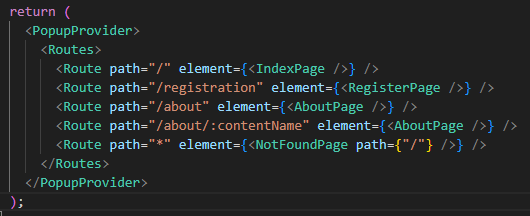
\includegraphics[width=0.7\textwidth]{zdj/index_router.png}
    \caption{Schemat routingu dla ogólnodostępnych stron w aplikacji.}
\end{figure}

MainRouter natomiast obsługuje zasoby, które są dostępne tylko dla zarejestrowanych i zweryfikowanych użytkowników. W tej części aplikacji przed uzyskaniem dostępu do stron, takich jak profil użytkownika, ranking czy gra online, aplikacja przeprowadza weryfikację, czy użytkownik jest odpowiednio zalogowany i posiada uprawnienia do korzystania z tych zasobów. Jeśli użytkownik nie spełnia wymogów autentykacji, zostaje przekierowany do odpowiednich stron, takich jak strona logowania czy rejestracji.
\begin{figure}[h!]
    \centering
    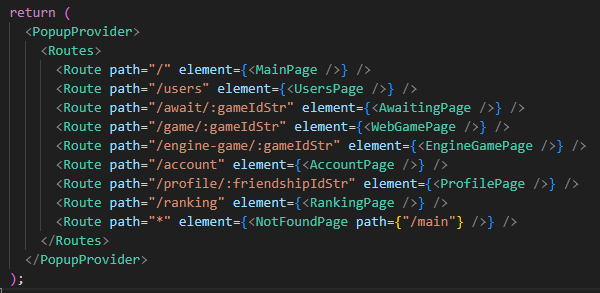
\includegraphics[width=0.7\textwidth]{zdj/main_router.png}
    \caption{Schemat routingu dla zasobów dostępnych tylko dla zalogowanych i zweryfikowanych użytkowników.}
\end{figure}

\newpage

\textbf{Autoryzacja}\\
Autoryzacja w MainRouterze polega na weryfikacji tokena użytkownika oraz stanu jego konta. Przy każdym wejściu na zasoby chronione, aplikacja najpierw sprawdza, czy w localStorage znajduje się token. Jeśli go brak, użytkownik jest przekierowywany do strony rejestracji. Następnie, jeśli token jest obecny, aplikacja sprawdza, czy adres e-mail użytkownika został zweryfikowany. W przypadku braku weryfikacji, użytkownik zostaje przekierowany do strony rejestracji z komunikatem o konieczności weryfikacji konta. Po pomyślnym zweryfikowaniu konta, aplikacja pobiera dane użytkownika, zapisuje je w localStorage i nawiązuje połączenie z serwisem gier. W przypadku jakichkolwiek problemów z autoryzacją, użytkownik jest również kierowany do strony rejestracji z odpowiednim komunikatem o błędzie.

\begin{figure}[h!]
    \centering
    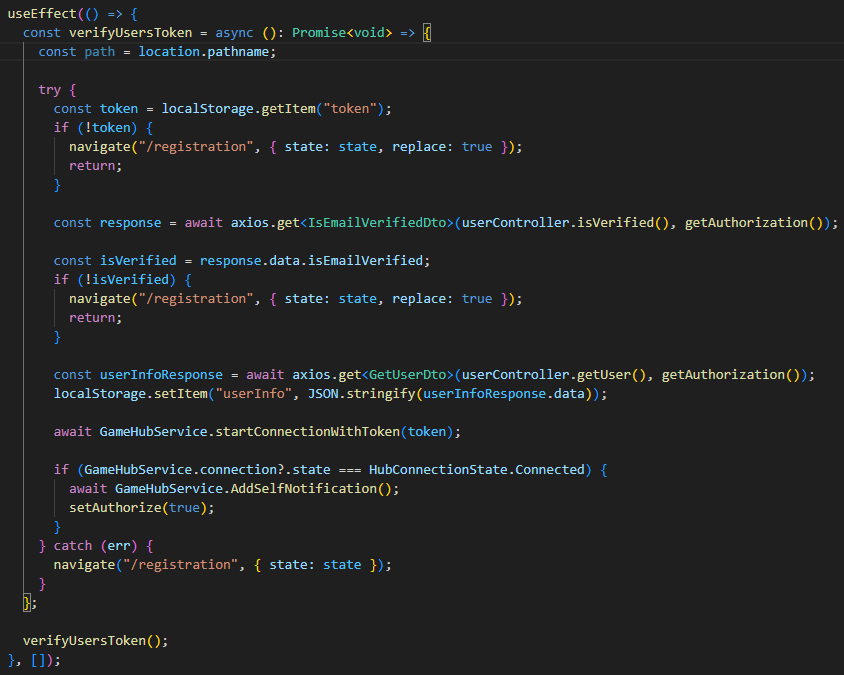
\includegraphics[width=1\textwidth]{zdj/mrouter_authorization.png}
    \caption{Fragment kodu pokazujący proces autoryzacji użytkownika.}
\end{figure}

\newpage
\subsubsection{Komponenty interfejsu użytkownika}

Aplikacja korzysta z dwóch głównych routerów, z których pierwszy obsługuje strony dostępne publicznie, które stanowią wstęp do pełnej aplikacji i są dostępne bez konieczności logowania, zapewniając użytkownikom możliwość zapoznania się z funkcjami platformy przed założeniem konta. Drugi natomiast zarządza stronami, które są dostępne tylko po zalogowaniu się użytkownika i obejmują pełną funkcjonalność aplikacji. Strony te wymagają uwierzytelnienia, aby zapewnić bezpieczeństwo danych użytkowników oraz personalizację doświadczenia, co pozwala na pełne wykorzystanie możliwości aplikacji, takich jak interakcja z innymi graczami czy dostosowywanie ustawień profilu.
\\\\

\textbf{Strona tytułowa (Index)}\\
Strona tytułowa stanowi pierwsze spotkanie użytkownika z aplikacją. Zawiera ona szereg sekcji, które mają na celu zaprezentowanie aplikacji w sposób przejrzysty i zachęcający do dalszej interakcji. Sekcje na tej stronie mogą obejmować ogólne wprowadzenie do gry w szachy, zasady gry, możliwość rozpoczęcia gry online lub offline, a także funkcje aplikacji, takie jak zarządzanie znajomymi, zaproszenia do gry, czy dostęp do rankingów. Celem tej strony jest zainteresowanie użytkownika, zrozumienie, czym jest aplikacja i zachęcenie go do rejestracji lub logowania.
\\

\textbf{Strona informacyjna (About)}\\
Strona informacyjna zawiera szczegółowe informacje na temat aplikacji, jej twórców, celu, zasad działania, jak również warunki korzystania z platformy i politykę prywatności. Jest to miejsce, gdzie użytkownicy mogą zapoznać się z pełnym opisem aplikacji, jej funkcji, zasadami bezpieczeństwa oraz wymaganiami. Dzięki tej stronie użytkownik zyskuje pełen obraz tego, czego może oczekiwać od aplikacji, a także jest informowany o zasadach korzystania z usługi.
\\

\textbf{Strona do rejestracji (Register)}\\
Strona rejestracji i logowania jest kluczowym komponentem, umożliwiającym użytkownikowi utworzenie konta, zalogowanie się lub przejście przez proces weryfikacji. Ta strona składa się z jednego okna, które zmienia się dynamicznie w zależności od podjętej akcji przez użytkownika. Może to obejmować różne stany, takie jak formularz rejestracji, formularz logowania lub okno informacyjne o konieczności weryfikacji konta po jego utworzeniu. Wszystkie te akcje są obsługiwane w ramach jednego komponentu, który dynamicznie przełącza widoki w zależności od wyboru użytkownika.
\\

\textbf{Strona główna (Main)}\\
Strona główna, dostępna zaraz po zalogowaniu, stanowi centrum nawigacji aplikacji. Z jej poziomu użytkownik może rozpocząć grę, zapoznać się z historią swoich poprzednich gier, a także przejść do innych sekcji, takich jak konto użytkownika, znajomi, ranking czy ustawienia. Strona ta pełni rolę wprowadzenia do pełnej funkcjonalności aplikacji, umożliwiając użytkownikowi szybki dostęp do najistotniejszych opcji. Oprócz rozpoczęcia nowych gier i przeglądania starych, użytkownik może również zapraszać znajomych do gry lub przejrzeć dostępne tryby rozgrywki.
\\

\textbf{Strona gry online (WebGame)}\\
Jest to komponent odpowiedzialny za rozgrywki online. Mechanizm gry w tym przypadku oparty jest na interakcji dwóch graczy, którzy mogą rywalizować ze sobą w czasie rzeczywistym. Gra jest synchronizowana na bieżąco za pomocą mechanizmów, takich jak SignalR, co pozwala na natychmiastowe przesyłanie danych o wykonanych ruchach i stanie gry między użytkownikami. Strona ta oferuje interfejs umożliwiający pełną interakcję z planszą szachową, a także daje możliwość korzystania z dodatkowych funkcji, takich jak czat czy podgląd statystyk. Wygląd strony jest zoptymalizowany pod kątem dynamicznej gry online, zapewniając użytkownikowi płynne doświadczenie.
\\

\textbf{Strona gry offline (EngineGame)}\\
Ten komponent odpowiada za tryb gry z komputerem, czyli tryb offline. W tym przypadku użytkownik gra przeciwko sztucznej inteligencji (AI), a rozgrywka jest realizowana w trybie offline, bez potrzeby połączenia z innym graczem. Mechanizmy gry różnią się od tych w trybie online, gdyż cała interakcja odbywa się tylko po stronie użytkownika i aplikacji, bez wymiany danych z zewnętrznymi źródłami. Strona EngineGame jest pod względem wyglądu podobna do strony WebGame, jednak w tym przypadku użytkownik nie ma możliwości zaproszenia znajomych do gry, a interakcja opiera się wyłącznie na grze z komputerem.
\\

\textbf{Strona konta użytkownika (Account)}\\
Strona konta użytkownika to miejsce, w którym użytkownik może przeglądać i edytować swój profil. Zawiera ona informacje na temat użytkownika, takie jak nazwa, e-mail, zdjęcie profilowe oraz inne szczegóły, które można zmieniać. Dodatkowo, użytkownik ma dostęp do ustawień konta, takich jak zmiana hasła czy preferencje dotyczące powiadomień. Strona ta zawiera również sekcję z podsumowaniem statystyk gracza – liczba wygranych gier, ranking, liczba rozegranych partii i inne osiągnięcia.
\\

\textbf{Strona zarządzania znajomymi (Users)}\\
Umożliwia ona użytkownikowi zarządzanie znajomymi i zapraszanie nowych osób do gry. Na tej stronie użytkownik może przeglądać swoich znajomych, wyszukiwać innych graczy, a także zapraszać ich do gry. Jest to także miejsce, gdzie można przeglądać historię zaproszeń i statusy graczy (czy są online, czy dostępni do gry). Użytkownik ma możliwość usuwania znajomych lub zatwierdzania nowych zaproszeń.
\\

\textbf{Strona profilu znajomego (Profile)}\\
Strona ta pozwala na podgląd profili innych użytkowników. Dzięki tej stronie użytkownik może zapoznać się z danymi innych graczy, ich statystykami, historią gier oraz osiągnięciami. Umożliwia to łatwiejsze nawiązanie kontaktu i zaproszenie do gry. Strona ta pełni funkcję informacyjną, pozwalając użytkownikowi lepiej poznać innych graczy i ich styl gry.
\\

\textbf{Strona rankingu (Ranking)}\\
Strona rankingu pokazuje aktualne rankingi graczy, zarówno na poziomie globalnym, jak i wśród znajomych. Użytkownik może przeglądać globalne rankingi, zobaczyć, jak plasuje się w porównaniu do innych graczy na całym świecie, jak również sprawdzić wyniki swoich znajomych. Ranking jest aktualizowany na bieżąco, odzwierciedlając wyniki wszystkich gier rozegranych w aplikacji. Dzięki temu użytkownicy mogą śledzić swoje postępy i starać się poprawić swoją pozycję w rankingu.
\\

\textbf{Strony ładowania (Loading)}\\
Aplikacja zawiera również strony ładowania, które są wyświetlane w sytuacjach, gdy użytkownik musi poczekać na załadowanie zasobów lub wykonanie operacji, takich jak pobieranie danych z serwera. Strony te pełnią rolę informacyjną i zapewniają użytkownikowi feedback na temat aktualnego stanu procesu, na przykład ładowania gry, oczekiwania na odpowiedź z serwera lub innych operacji wymagających czasu.


\newpage
\subsubsection{Zarządzanie stanem aplikacji}
Zarządzanie stanem aplikacji w projekcie opiera się na elastycznym wykorzystaniu kilku mechanizmów w zależności od charakteru stanu i jego zastosowania. Dzięki temu aplikacja jest w stanie skutecznie zarządzać zarówno lokalnym stanem komponentów, jak i bardziej złożonymi danymi związanymi z rozgrywką, zapewniając płynność i responsywność działania aplikacji w grze w szachy.

\begin{itemize}
    \item \textbf{Zarządzanie stanem lokalnym:} Do zarządzania stanem lokalnym, który jest związany z pojedynczymi komponentami, wykorzystywane jest useState. Tego typu stan przechowuje dane dotyczące interakcji użytkownika z interfejsem, na przykład wybór gry, filtrowanie wyników czy przechowywanie tymczasowych danych. Stan ten jest zmieniany w odpowiedzi na działania użytkownika lub pobieranie danych z serwera.
    \item \textbf{Zarządzanie bardziej złożonym stanem:} W przypadku bardziej skomplikowanego stanu, takiego jak stan gry, używa się useReducer. Ta technika pozwala na lepsze zarządzanie złożonymi i dynamicznymi danymi, takimi jak aktualny stan rozgrywki, ruchy graczy, status gry czy zmiany na planszy. Dzięki zastosowaniu reducerów możliwe jest łatwe śledzenie zmian stanu oraz utrzymywanie porządku w logice aplikacji, szczególnie w sytuacjach, gdy wiele akcji może wpływać na jeden obiekt stanu.
    \item \textbf{Globalny stan aplikacji:} Aby zarządzać danymi, które muszą być dostępne w wielu częściach aplikacji, wykorzystywany jest globalny stan oparty na useContext i createContext. Dzięki temu możliwe jest centralne przechowywanie i udostępnianie informacji, które są wykorzystywane w różnych miejscach aplikacji.
    \item \textbf{Przechowywanie danych w localStorage:} Aplikacja wykorzystuje także localStorage do przechowywania niektórych danych, takich jak informacje o użytkowniku czy tokeny logowania. Dzięki temu dane te pozostają dostępne pomiędzy sesjami użytkownika, nawet po odświeżeniu strony lub zamknięciu aplikacji. localStorage zapewnia trwałość przechowywanych danych, co zwiększa komfort użytkownika, umożliwiając m.in. automatyczne logowanie się lub kontynuowanie gry bez potrzeby ponownego logowania.
    \item \textbf{Komunikacja w czasie rzeczywistym z użyciem SignalR:}
    W aplikacji szachowej, gdzie interakcja dwóch graczy musi odbywać się w czasie rzeczywistym, wykorzystano SignalR do synchronizacji stanu gry między graczami. Po wykonaniu ruchu przez jednego gracza, aplikacja natychmiastowo informuje drugiego gracza o zmianach, co pozwala na płynne i bieżące aktualizowanie stanu gry w czasie rzeczywistym. Dzięki SignalR, obaj gracze widzą zmiany na planszy bez opóźnień i mogą natychmiastowo reagować na ruchy przeciwnika.
\end{itemize}

\newpage
\subsubsection{Mechanizm gry w szachy}
Proces zarządzania przebiegiem gry w szachy w aplikacji opiera się na dynamicznym śledzeniu i aktualizowaniu stanu gry w odpowiedzi na interakcje użytkownika. Cała procedura składa się z kilku etapów, które są ze sobą ściśle powiązane, aby zapewnić płynność rozgrywki i zgodność z zasadami szachów.
\\\\

\textbf{Pobranie stanu gry}\\
Pierwszym krokiem jest pobranie aktualnego stanu gry z bazy danych, co pozwala na załadowanie pozycji wszystkich figur na planszy w chwili, gdy użytkownik wchodzi na stronę gry. Stan gry obejmuje pozycję wszystkich figur, informacje o graczach oraz inne dane związane z przebiegiem partii (np. liczba wykonanych ruchów, stan szachowy). Te dane są następnie zapisywane w bieżącym stanie aplikacji, co umożliwia dalsze operacje na szachownicy.
\\
\textbf{Mapowanie pozycji na macierz szachownicy}\\
Po załadowaniu stanu gry, aplikacja przekształca dane dotyczące pozycji figur w odpowiednią macierz, która reprezentuje szachownicę. Dzięki temu można łatwo manipulować danymi i aktualizować widok planszy. Każda figura jest przypisana do konkretnych współrzędnych na planszy, co umożliwia jej wyświetlenie w odpowiednim miejscu. Mapowanie pozycji do macierzy pozwala również na łatwiejsze śledzenie możliwych ruchów dla każdej figury.
\\
\textbf{Kontrolowanie pól}\\
Aplikacja następnie tworzy listy kontrolowanych pól dla obu graczy. Każde pole, na którym może spaść bicie, jest uwzględniane w tych listach. Ponadto, ważnym elementem jest zapewnienie, że król nie może wejść na pole, które jest zagrożone przez przeciwnika (czyli nie może stanąć na polu, które może zostać zaatakowane przez przeciwnika w kolejnej turze). Lista kontrolowanych pól jest dynamicznie aktualizowana po każdym ruchu, aby zapewnić prawidłową grę.
\\
\textbf{Sprawdzanie szacha}\\
Kolejnym istotnym etapem jest sprawdzenie, czy w danej chwili istnieje szach. Szach to sytuacja, w której król jednego z graczy znajduje się pod bezpośrednim atakiem przeciwnika, co oznacza, że gracz musi podjąć działania w celu ochrony swojego króla. Jeśli występuje szach, aplikacja identyfikuje wszystkie pola, które biorą udział w szachu, co pozwala na zmuszenie gracza do podjęcia odpowiednich działań. Oznacza to, że gracz nie może swobodnie poruszać innymi figurami, a ruchy, które mogłyby zwiększyć zagrożenie, są blokowane.
\\
\textbf{Wyczyszczenie wcześniejszych wyborów}\\
Po wykonaniu każdego ruchu lub interakcji z użytkownikiem, aplikacja wyczyści wszelkie wcześniejsze wybory dokonywane przez gracza. Na przykład, jeśli użytkownik wybrał figurę, a następnie nie wybrał jej nowej lokalizacji, poprzedni wybór zostaje anulowany. Zapewnia to, że nie pozostają żadne błędne lub nieaktualne dane, które mogłyby wpłynąć na dalszą grę.
\\
Zanim gracz będzie mógł dokonać wyboru figury, aplikacja sprawdza, czy istnieje jakikolwiek możliwy ruch, który można wykonać. Jeśli żaden ruch nie jest możliwy (np. w przypadku "matu" lub "patu"), gra zostaje zakończona. W przypadku matu (zamatowanie króla) jedna ze stron wygrywa, natomiast w przypadku pata (niemożliwość wykonania ruchu, ale król nie jest w szachu) gra kończy się remisem. Aplikacja automatycznie wykrywa te sytuacje i odpowiednio kończy grę.
\\
\textbf{Wybór figury i koordynat}\\
Po sprawdzeniu dostępnych ruchów, gracz może wybrać figurę, którą chce ruszyć. Po dokonaniu wyboru, aplikacja zapisuje wybraną figurę oraz jej koordynaty na planszy. Następnie, użytkownik wybiera pole, na które chce wykonać ruch. W tym momencie aplikacja uruchamia procedurę obliczania wszystkich możliwych ruchów, jakie figura może wykonać na podstawie aktualnych zasad gry (np. ruchy dla pionka, wieży, gońca, itp.).
\\
\textbf{Podświetlanie dostępnych pól}\\
Po obliczeniu dostępnych ruchów, aplikacja aktualizuje widok planszy, podświetlając odpowiednie pola, na które wybrana figura może się poruszyć. Dzięki temu użytkownik ma pełną widoczność swoich opcji i może łatwiej podjąć decyzję. Podświetlone są tylko te pola, które są zgodne z zasadami ruchów danej figury, co eliminuje możliwość wykonania błędnego ruchu.
\\
\textbf{Wykonanie ruchu}\\
Po dokonaniu wyboru pola przez użytkownika, aplikacja sprawdza, czy ruch jest dozwolony. Jeśli tak, wykonuje ruch, przenosząc figurę na nowe pole. Jeżeli ruch jest nielegalny (np. figura nie może poruszyć się na to pole zgodnie z zasadami gry), aplikacja anuluje wybór i pozwala graczowi ponownie wybrać figurę i cel ruchu.
\\
\textbf{Aktualizacja stanu gry}\\
Po wykonaniu ruchu aplikacja zapisuje nowy stan gry w bazie danych, co pozwala na kontynuowanie gry od tego punktu w przyszłości. Zmiany w stanie gry obejmują aktualizację pozycji figur, liczbę wykonanych ruchów oraz ewentualne zmiany w statusie gry (np. wprowadzenie szacha, matu lub pata). Dzięki temu stan gry jest synchronizowany i zabezpieczony na wypadek przerwania gry lub ponownego załadowania strony.
\\
\textbf{Powiadomienie drugiego gracza}\\
Na końcu, po zapisaniu zmian w bazie, aplikacja powiadamia drugiego gracza o wykonanym ruchu, aby umożliwić mu podjęcie swojej tury. Powiadomienie jest realizowane za pomocą technologii SignalR, która zapewnia natychmiastową synchronizację stanu gry pomiędzy graczami. To kluczowy element umożliwiający grę online w czasie rzeczywistym, gdzie każdy ruch jednego gracza jest natychmiastowo widoczny dla drugiego gracza.
\\\\
Poniżej przedstawiony został diagram blokowy ilustrujący proces działania mechanizmu gry w szachy. Diagram prezentuje kolejne etapy, począwszy od inicjalizacji stanu gry, przez interakcje użytkownika, aż po synchronizację stanu gry pomiędzy graczami. Każdy etap jest odzwierciedleniem opisanego wcześniej przebiegu logiki gry, uwzględniając kluczowe decyzje i akcje, takie jak obliczanie możliwych ruchów, weryfikacja poprawności ruchu czy zakończenie gry.

\newpage

\begin{figure}[h!]
    \centering
    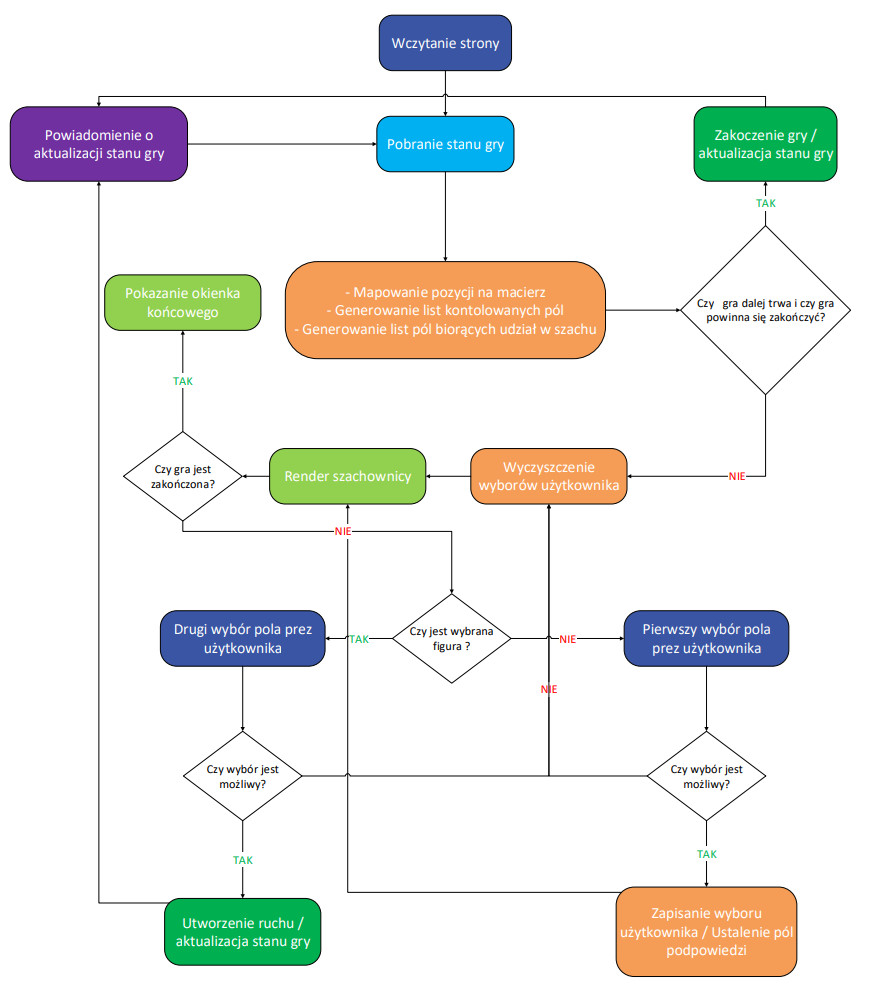
\includegraphics[width=1\textwidth]{zdj/diagram_gry.png}
    \caption{Diagram blokowy mechanizmu gry w szachy.}
\end{figure}

\newpage
\subsubsection{Kluczowe aspekty gry}
\textbf{Pozycja FEN}\\
Pozycja FEN (Forsyth-Edwards Notation) to sposób zapisywania aktualnej sytuacji na szachownicy, który pozwala na jednoznaczne odtworzenie pozycji w dowolnym momencie gry. Zawiera wszystkie istotne informacje o rozmieszczeniu figur, kolorze gracza, który ma wykonać ruch, stanie roszady, liczbie ruchów od ostatniego bicia lub ruchu pionkiem, oraz liczbie pełnych ruchów.
\\\\
W kontekście aplikacji, zapis FEN jest wykorzystywany do przechowywania stanu gry w bazie danych. Dzięki temu możliwe jest zapisanie aktualnej pozycji w dowolnym momencie, a następnie jej odczytanie i przywrócenie, co pozwala na wznowienie gry lub analizę wcześniejszych stanów.

\begin{center}
    \texttt{rnbqkbnr/pppppppp/8/8/8/8/PPPPPPPP/RNBQKBNR w KQkq - 0 1}
\end{center}

Przedstawioną przykładową pozycje można podzielić kolejno na części oznaczające:
\begin{itemize}
    \item Rozmieszczenie figur na szachownicy, z użyciem liter oraz liczb wskazujących puste pola.
    \item Kolor gracza, który ma wykonać ruch.
    \item Informacja o dostępności roszady dla obu graczy.
    \item Pozycja pionka, który może wykonać ruch en passant.
    \item Liczba ruchów od ostatniego bicia lub ruchu pionkiem.
    \item Liczba pełnych ruchów.
\end{itemize}

\textbf{Macierz szachownicy}\\
W pierwszej części zapisu pozycji FEN znajdują się informacje o rozmieszczeniu figur na szachownicy. Program przetwarza ten zapis, mapując go na macierz 8x8, co umożliwia łatwiejsze operowanie na koordynatach. Dzięki tej mapie, każdy element (pole) szachownicy może być odwoływany za pomocą indeksów, co ułatwia implementację ruchów, sprawdzanie stanu gry, a także operacje na poszczególnych figurach. Na przykład, każdemu polu szachownicy przypisane są współrzędne (x, y), gdzie x to numer kolumny (od A do H), a y to numer wiersza (od 1 do 8). Taki sposób reprezentacji umożliwia wygodną manipulację i analizowanie stanu gry.

\begin{figure}[h!]
    \centering
    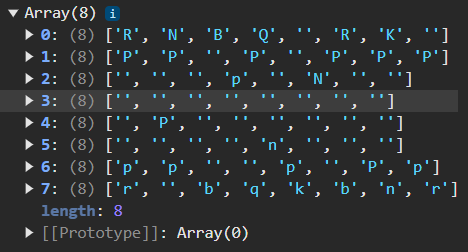
\includegraphics[width=0.7\textwidth]{zdj/matrix.png}
    \caption{Przykładowa macierz pozycji gry.}
\end{figure}

\newpage
\textbf{Szach}\\
Jest to sytuacja w grze w szachy, w której król jednego z graczy znajduje się pod atakiem przeciwnika, co oznacza, że przeciwnik mógłby zbić króla w swoim kolejnym ruchu, gdyby nie został on obroniony. W odpowiedzi na szach gracz musi podjąć ruch eliminujący zagrożenie dla króla. Istnieją trzy możliwe sposoby na uniknięcie szacha:

\begin{itemize}
    \item Przesunięcie króla na pole, które nie jest zagrożone przez przeciwnika.
    \item Zasłonięcie króla inną figurą, jeśli zagrożenie pochodzi z linii działania.
    \item Zbicie atakującej figury, jeśli jest to możliwe.
\end{itemize}

Nieodpowiedzenie na szach jest niedozwolone, ponieważ król nigdy nie może pozostawać na szachowanym polu. Jeśli gracz nie ma możliwości zneutralizowania szacha, partia kończy się matem.
\\\\
W projekcie sytuacja szachu została rozwiązana poprzez tworzenie dwóch par list. Pierwsza z nich obejmuje pola kontrolowane, czyli te, na które figury przeciwnika mogą wykonać bicie. Pola te są wykorzystywane do zapewnienia, że król nie może wejść na pole, na którym byłby zagrożony zbiciem, a także do sprawdzania, czy aktualnie znajduje się w szachu, jeśli stoi na takim polu.
\\\\
Druga para to listy pól biorących udział w szachu. Obejmują one pole zajmowane przez figurę szachującą oraz wszystkie pola, przez które szach jest „przekazywany” (na przykład w przypadku szachów liniowych, takich jak atak wieży, gońca czy hetmana). Pola te są wykorzystywane do ograniczenia możliwych ruchów innych figur, tak aby uniemożliwić wykonanie ruchu niezapewniającego zakończenia szachu. Dzięki temu mechanizmowi tylko ruchy ratujące króla są dopuszczalne w trakcie szachu, co w pełni odwzorowuje zasady gry w szachy.

\vspace{1cm}

\begin{minipage}[t]{0.45\textwidth} 
    \vspace{0pt} 
    \centering 
    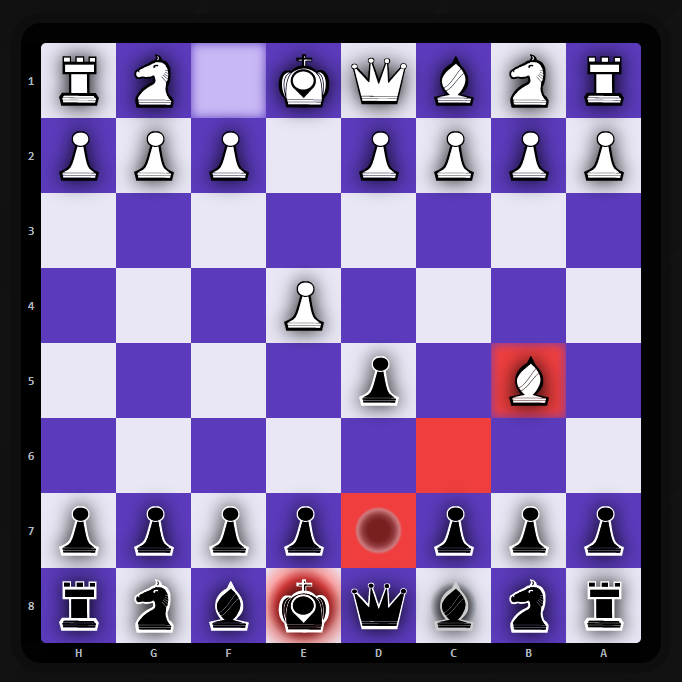
\includegraphics[width=\linewidth]{zdj/check_areas.png} 
    Wizualizacja pól szachu.
\end{minipage} 
\hfill 
\begin{minipage}[t]{0.45\textwidth} 
    \vspace{0pt} 
    \centering 
    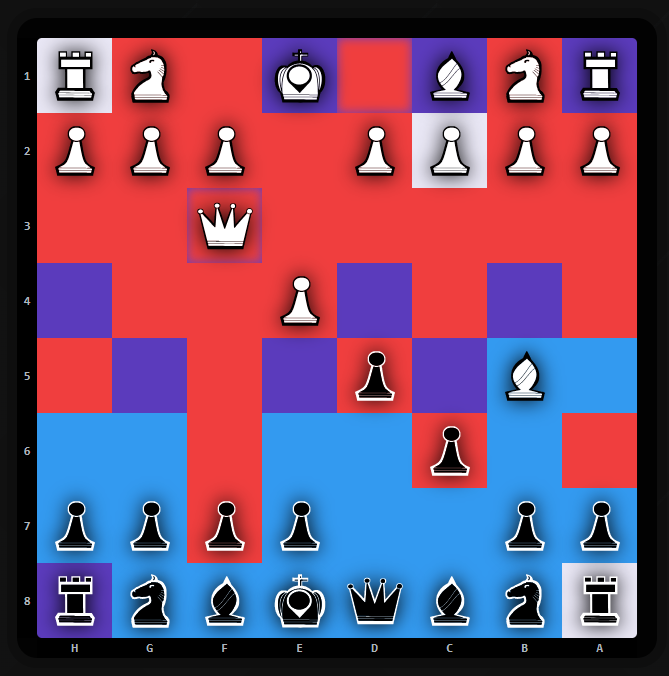
\includegraphics[width=\linewidth]{zdj/controlled_areas.png} 
    Wizualizacja kontrolowanych pól.
\end{minipage}

\newpage
\textbf{Mat i Pat}\\
W szachach mat i pat to dwie podstawowe sytuacje kończące grę. Mat oznacza, że król jednego z graczy jest w szachu i nie ma żadnych dostępnych ruchów, które mogłyby go uratować. Gra kończy się zwycięstwem przeciwnika. Pat, z kolei, ma miejsce wtedy, gdy gracz nie jest w szachu, ale nie ma żadnego legalnego ruchu, który mógłby wykonać. W takiej sytuacji gra kończy się remisem.
\\\\
W implementacji gry, te dwa scenariusze są rozwiązywane poprzez sprawdzanie dostępnych ruchów dla gracza, który jest aktualnie w turze. Gdy gracz próbuje wykonać ruch, najpierw sprawdzane jest, czy istnieje jakikolwiek możliwy ruch. Jeśli gracz nie ma żadnego dostępnego ruchu, program przechodzi do dalszej analizy.
\\\\
Jeśli po sprawdzeniu okazuje się, że gracz nie ma żadnych możliwych ruchów, następnie sprawdzane jest, czy jego król znajduje się w szachu. Jeśli król jest w szachu, oznacza to, że gra kończy się matem, a zwycięzcą zostaje przeciwnik. W przeciwnym przypadku, jeżeli gracz nie ma ruchu, ale jego król nie jest w szachu, oznacza to, że mamy do czynienia z patem, a gra kończy się remisem.

\begin{figure}[h!]
    \centering
    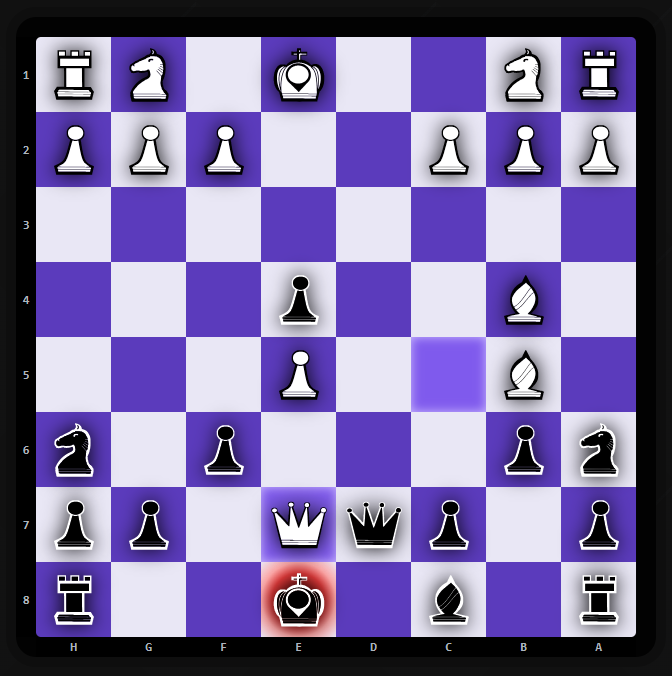
\includegraphics[width=0.7\textwidth]{zdj/checkmate.png}
    \caption{Przykładu zakończenia gry matem.}
\end{figure}

Tego rodzaju mechanizm pozwala na prawidłowe rozpoznawanie zakończenia gry w sytuacjach, kiedy gracz nie ma już możliwości wykonania ruchu, a także zapewnia zgodność z zasadami gry.

\newpage
\textbf{Pin (Przypięcie)}\\
W szachach ruchy dzielą się na liniowe i nieliniowe. Liniowe obejmują ruchy prostoliniowe oraz diagonalne. Figury poruszające się liniowo to wieża, goniec i hetman. Nieliniowe ruchy charakteryzują się bardziej złożonymi trajektoriami, jak w przypadku skoczka.
\\\\
W implementacji gry mechanizm wykrywania pina opiera się na analizie linii prostych i diagonalnych między królem a wybraną figurą. Sprawdzane jest, czy w tej samej linii znajduje się figura przeciwnika, zdolna do wykonania ruchu liniowego (wieża, goniec lub hetman). Jeśli taka sytuacja występuje, to ruchy wybranej figury są ograniczone do kierunku pina – figura może się poruszać jedynie w linii między królem a figurą przeciwnika, o ile jej natura pozwala na ruch w tym kierunku.
\\\\
Mechanizm pina może być zastosowany wyłącznie przez figury poruszające się liniowo: wieżę, gońca i hetmana. Ich zdolność do kontroli dużej liczby pól sprawia, że pin jest jednym z kluczowych narzędzi taktycznych w szachach, zarówno w ataku, jak i w obronie. Implementacja tego mechanizmu zapewnia zgodność z regułami gry, jednocześnie dodając istotną warstwę realizmu i taktyki do systemu.

\vspace{1cm}
\begin{minipage}[t]{0.45\textwidth} 
    \vspace{0pt} 
    \centering 
    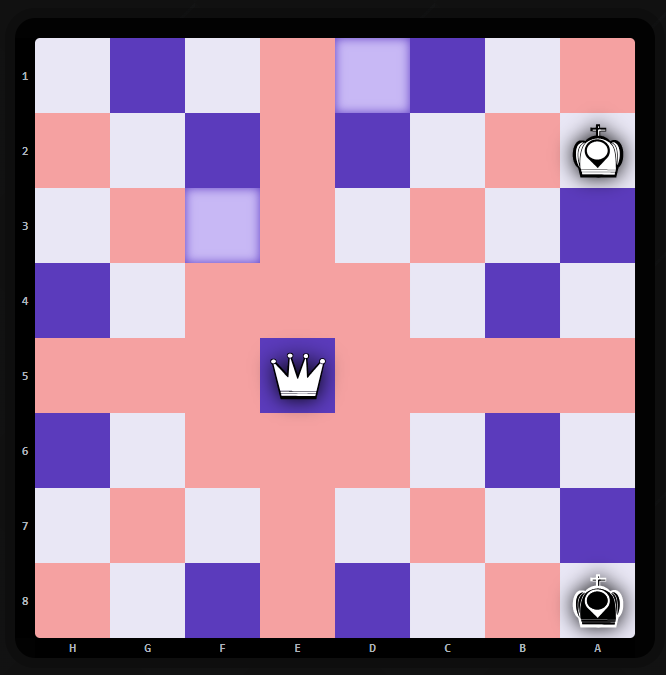
\includegraphics[width=\linewidth]{zdj/linear.png} 
    Wizualizacja ruchów liniowych na przykładzie ruchów hetmana.
\end{minipage} 
\hfill 
\begin{minipage}[t]{0.45\textwidth} 
    \vspace{0pt} 
    \centering 
    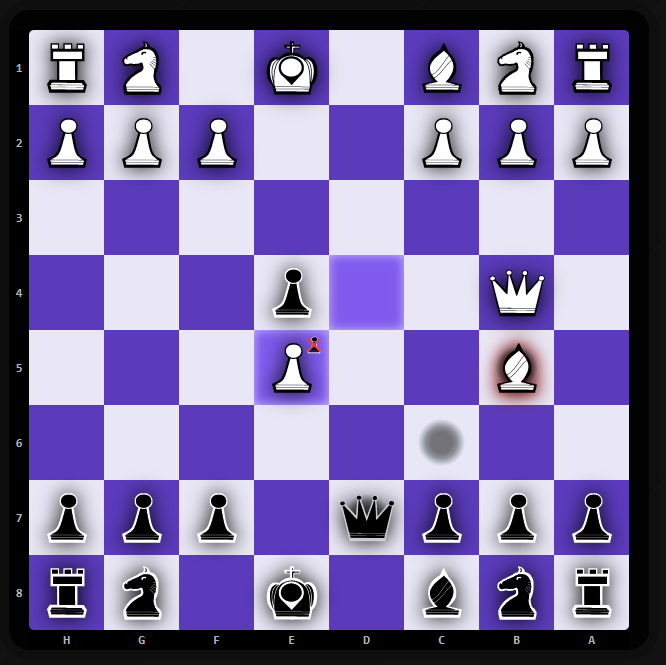
\includegraphics[width=\linewidth]{zdj/pin.png} 
    Wizualizacja przykładowego pinu na hetmanie.
\end{minipage}
\vspace{1cm}

Ponadto, w kontekście końca gry, piny odgrywają istotną rolę w decydowaniu, czy gra powinna się zakończyć. Mogą one ograniczać dostępne ruchy i zmuszać gracza do wykonania ruchu, który może prowadzić do matu lub patu. Gdy pionki, figury lub król zostają "przypięte", ich możliwości manewru są ograniczone, co znacząco wpływa na dalszy przebieg rozgrywki. Dodatkowo, jeśli przypięta figura nie może się poruszyć, może to prowadzić do sytuacji, w której gracz nie ma wystarczającej ilości ruchów do obrony, co przyczynia się do ostatecznego zwycięstwa.

\newpage
\textbf{Ruchy specjalne}\\
Ruchy specjalne w szachach, są przetwarzane za pomocą zapisanych specjalnych stanów w bazie danych. Na przykład, system przechowuje informacje o tym, czy roszada może zostać wykonana, bazując na wcześniejszych ruchach króla i wieży oraz innych warunkach, takich jak brak przeszkód na drodze. Ponadto, wykorzystywane są stałe wartości, takie jak pozycja pionka (tzw. ranga), które decydują o tym, kiedy dochodzi do promocji pionka, czy też kiedy pionek ma możliwość poruszenia się o dwa pola do przodu.

\vspace{1cm}
\begin{minipage}[t]{0.6\textwidth} 
    \vspace{0pt} 
    \raggedright 
    \textbf{Roszada}\\
    Roszada jest specjalnym ruchem, który polega na jednoczesnym przesunięciu króla i wieży. Aby ten ruch był możliwy, muszą być spełnione określone warunki, takie jak brak wcześniejszych ruchów króla i wieży oraz brak przeszkód między nimi. Dodatkowo, król nie może być w szachu ani przechodzić przez pole, które jest zagrożone.
\end{minipage} 
\hfill 
\begin{minipage}[t]{0.3\textwidth} 
    \vspace{0pt} 
    \centering 
    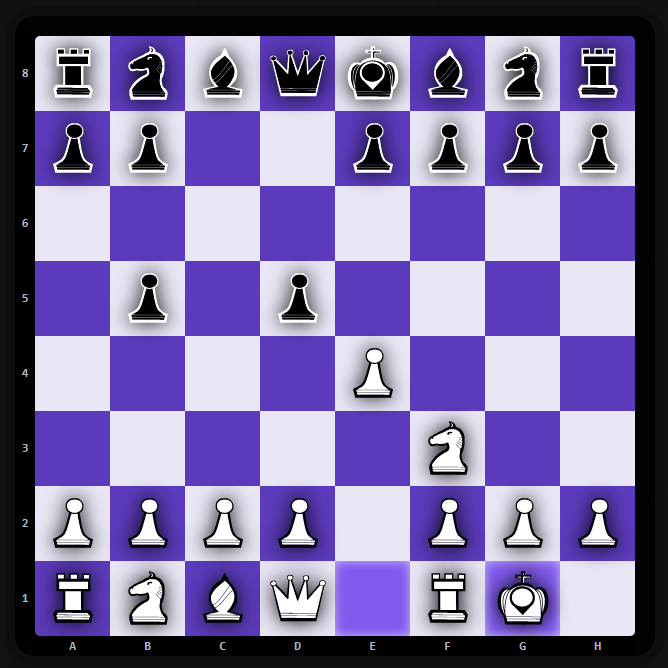
\includegraphics[width=\linewidth]{zdj/castling.png} 
\end{minipage}
\vspace{1cm}
\begin{minipage}[t]{0.3\textwidth} 
    \vspace{0pt} 
    \centering 
    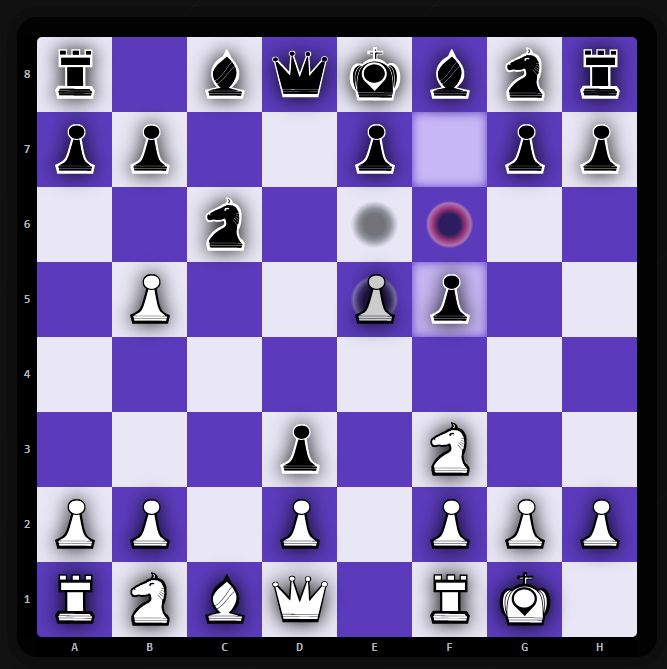
\includegraphics[width=\linewidth]{zdj/enpassant.png} 
\end{minipage} 
\hfill 
\begin{minipage}[t]{0.6\textwidth} 
    \vspace{0pt} 
    \raggedright 
    \textbf{Bicie w przelocie}\\
    Bicie w przelocie jest specyficznym przypadkiem, który może wystąpić, gdy pionek przeciwnika poruszy się o dwa pola do przodu, a nasz pionek znajduje się na sąsiednim polu. W takim przypadku nasz pionek może zbić pionka przeciwnika, jakby poruszył się tylko o jedno pole. System zapisuje koordynat, na którym może paść to bicie w stanie gry.
\end{minipage}
\vspace{1cm}
\begin{minipage}[t]{0.6\textwidth} 
    \vspace{0pt} 
    \raggedright 
    \textbf{Promocja pionka}\\
    Promocja pionka ma miejsce, gdy pionek dotrze do ostatniej linii planszy. Wtedy gracz ma możliwość wymiany pionka na inną figurę, najczęściej na hetmana, ale także na wieżę, gońca lub skoczka. Promocja jest obsługiwana przez system na podstawie pozycji pionka na planszy, czyli tzw. rangi, która determinuje moment jej wykonania.
\end{minipage} 
\hfill 
\begin{minipage}[t]{0.3\textwidth} 
    \vspace{0pt} 
    \centering 
    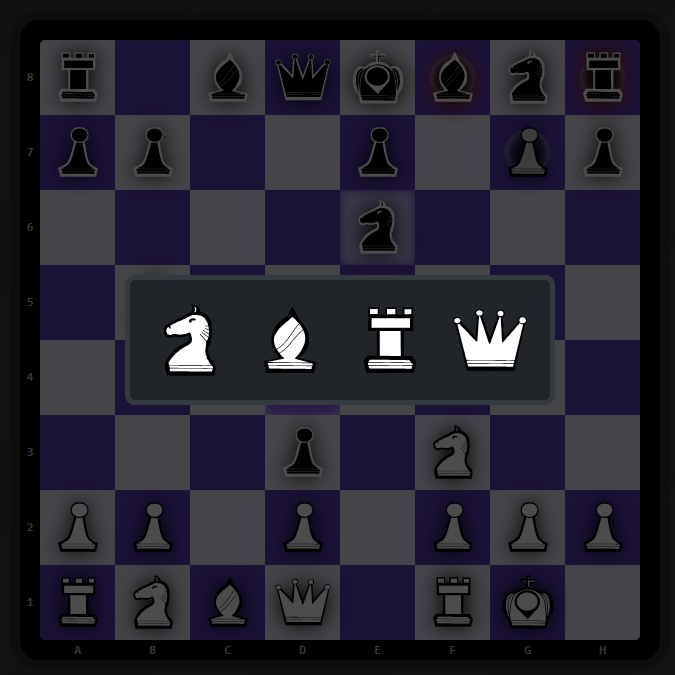
\includegraphics[width=\linewidth]{zdj/promotion.png} 
\end{minipage}

\newpage
\textbf{Pozostałe zasady końca gry}\\
W szachach istnieje kilka innych zasad, które mogą prowadzić do zakończenia gry przed standardowym zwycięstwem lub remisem. Oprócz klasycznego szacha-mata, są to zasady, które umożliwiają ogłoszenie remisu, nawet jeśli nie ma bezpośredniego zagrożenia dla króla. System ten wymaga od aplikacji precyzyjnego śledzenia przebiegu gry oraz różnych warunków, które mogą prowadzić do remisu. Oto szczegóły niektórych z tych zasad:


\begin{itemize}
    \item \textbf{Zasada trzykrotnego powtórzenia pozycji}\\
    Zasada ta pozwala ogłosić remis, jeśli ta sama pozycja na szachownicy wystąpiła trzykrotnie podczas gry, pod warunkiem, że pozycje te miały tę samą możliwość wykonania ruchu. W programie realizuje się to przez zapisanie wszystkich wykonanych ruchów oraz ich stanów w bazie danych. Program porównuje zapisaną historię i sprawdza, czy dana pozycja pojawiła się już co najmniej trzykrotnie. Jeśli tak, gra kończy się remisem.
    \item \textbf{Zasada 50 ruchów}\\
    Zasada 50 ruchów oznacza, że jeśli przez 50 kolejnych ruchów nie została wykonana żadna akcja, taka jak ruch pionka lub bicie figury, to gra kończy się remisem. W aplikacji ten stan jest śledzony za pomocą specjalnej zmiennej, która liczy tzw. "halfmove" (połowa ruchu). Zwiększa się ona o 1 za każdym razem, gdy nie został wykonany ruch pionka lub nie doszło do bicia. Jeśli liczba ta osiągnie 50, program uznaje, że zasada została spełniona i gra kończy się remisem. Jeśli w tym czasie wykonany zostanie ruch pionka lub dojdzie do bicia, licznik jest zerowany.
    \item \textbf{Niewystarczający ilość materiału}\\
    Jeśli na szachownicy nie ma wystarczającej ilości figur, aby móc wykonać mat, gra kończy się remisem. Na przykład, jeśli jeden z graczy ma tylko króla, a drugi gracz ma jedynie króla i jakąkolwiek inną figurę, nie będzie już możliwe zrealizowanie matu. W takim przypadku aplikacja analizuje całą planszę i sprawdza, czy występuje wystarczający materiał do wykonania matu. Jeżeli materiał jest niewystarczający, program ogłasza remis.
\end{itemize}

\textbf{Upłynięcie czasu}\\
W przypadku gry z czasem, aplikacja śledzi czas pozostały dla obu graczy i przechowuje te informacje w bazie danych. Czas jest odliczany dla każdego gracza indywidualnie, a po wykonaniu ruchu przez jednego z graczy, zegar zostaje zaktualizowany. Czas jest inkrementowany na podstawie zadanego interwału, który może być ustalony na początku gry. Kiedy jeden gracz wykonuje ruch, czas zostaje zaktualizowany o odpowiedni inkrement, a zegar drugiego gracza zaczyna odliczać swój czas. Cały proces jest realizowany poprzez zapisywanie stanu czasu w bazie danych oraz bieżące odliczanie dla aktywnego gracza. Jeśli czas któregokolwiek z graczy dobiegnie końca, gra automatycznie kończy się, a przegrany zostaje ogłoszony przegranym z powodu przekroczenia czasu. Tego typu funkcjonalność jest szczególnie przydatna w trybach szybkich gier, gdzie gracze mają określoną ilość czasu na wykonanie swoich ruchów.

\newpage
\subsubsection{Wykorzystane biblioteki}

\begin{itemize} 
    \item \textbf{react} i \textbf{react-dom}: React to biblioteka do tworzenia dynamicznych komponentów UI, a react-dom pozwala na renderowanie tych komponentów w DOM, integrując aplikację React z przeglądarką. 
    \item \textbf{typescript}: Typowanie statyczne dla JavaScript, które pomaga unikać błędów w kodzie oraz poprawia jego skalowalność.
    \item \textbf{@microsoft/signalr}: Biblioteka umożliwiająca komunikację w czasie rzeczywistym między aplikacjami frontendowymi a serwerem. Jest kluczowa do implementacji funkcji czatu, powiadomień lub innych aplikacji wymagających bieżącej wymiany danych w czasie rzeczywistym.
    \item \textbf{axios} i \textbf{msw}: Axios to klient HTTP do wysyłania zapytań do API, a MSW umożliwia mockowanie tych zapytań w trakcie rozwoju lub testowania aplikacji bez potrzeby aktywnego backendu. 
    \item \textbf{history} i \textbf{react-router-dom}: History umożliwia zarządzanie historią przeglądarki, a react-router-dom korzysta z tej biblioteki do obsługi routingu i nawigacji w aplikacjach SPA. 
    \item \textbf{jsonwebtoken} i \textbf{jwt-decode}: Biblioteki związane z uwierzytelnianiem. `jsonwebtoken` służy do tworzenia i weryfikacji tokenów JWT, które są używane do autoryzacji użytkowników, a `jwt-decode` umożliwia dekodowanie tych tokenów, pozwalając na ekstrakcję danych, takich jak dane użytkownika lub czas wygaśnięcia tokenu.
    \item \textbf{guid-typescript} i \textbf{uuid}: Obie biblioteki umożliwiają generowanie unikalnych identyfikatorów, które mogą być używane w aplikacjach do identyfikowania elementów, sesji lub użytkowników. 
    \item \textbf{vite} i \textbf{vitest}: Vite to bundler i serwer deweloperski, który wspiera nowoczesne technologie, a vitest to framework testowy zoptymalizowany pod kątem ekosystemu Vite, umożliwiający szybkie uruchamianie testów jednostkowych. 
    \item \textbf{@testing-library/dom} i \textbf{@testing-library/react}: Biblioteki do testowania DOM i komponentów React, umożliwiające tworzenie testów jednostkowych i integracyjnych w aplikacjach frontendowych. 
    \item \textbf{eslint} i \textbf{@eslint/js}: Narzędzia do statycznej analizy kodu w celu zapewnienia jakości i spójności kodu JavaScript, zgodnie z określonymi zasadami. 
    \item \textbf{stylelint}: Narzędzie do analizy jakości CSS i SCSS, zapewniające porządek w kodzie stylów. 
    \item \textbf{sass} i \textbf{scss}: Obie biblioteki to preprocesory CSS, gdzie SCSS jest bardziej zbliżoną do standardowego CSS wersją SASS. Używa się ich do organizowania i modularnego pisania stylów. 
\end{itemize}

\newpage
\section{Instrukcja obsługi}
\subsection{Strona startowa}
Strona tytułowa aplikacji do gry w szachy została zaprojektowana jako intuicyjny i funkcjonalny punkt startowy dla użytkowników. Umieszczono na niej wszystkie kluczowe elementy, które pozwalają na łatwe rozpoczęcie korzystania z platformy. W górnej części strony znajdują się przyciski umożliwiające logowanie oraz rejestrację, co pozwala zarówno nowym użytkownikom, jak i tym posiadającym konto na szybki dostęp do zasobów aplikacji.
\\\\
Centralna część strony prezentuje krótki opis funkcjonalności aplikacji. Zwrócono uwagę na najważniejsze elementy, takie jak możliwość gry online z innymi użytkownikami, rozbudowane narzędzia treningowe, tryb rozwiązywania łamigłówek szachowych oraz funkcje organizowania i uczestnictwa w turniejach. Wszystko to ma na celu wprowadzenie użytkownika w możliwości, jakie oferuje aplikacja, oraz zachęcenie do eksplorowania dostępnych funkcji.
\\\\
Na stronie znajduje się również sekcja umożliwiająca przejście do bardziej szczegółowego opisu zawartości aplikacji. Dzięki niej można zapoznać się z opisem poszczególnych funkcji oraz dowiedzieć się więcej o opcjach gry i trybach nauki. Dodatkowo zamieszczono odnośnik do działu FAQ, w którym zebrano odpowiedzi na najczęściej zadawane pytania, ułatwiając użytkownikom szybkie rozwiązanie ewentualnych wątpliwości.
\\\\
Całość zaprojektowano w sposób przejrzysty i estetyczny, aby zapewnić pozytywne pierwsze wrażenie oraz łatwość w poruszaniu się po stronie. Strona tytułowa pełni rolę wizytówki aplikacji, jednocześnie oferując dostęp do najważniejszych zasobów i funkcji.

\begin{figure}[h!]
    \centering
    
\includegraphics[width=1\textwidth]{zdj/ins_hero.png}
    \caption{Widok strony startowej.}
\end{figure}

\newpage
\subsection{Strona rejestracji}
Strona rejestracji w aplikacji łączy w sobie wszystkie kluczowe funkcje niezbędne do zarządzania kontem użytkownika. Pozwala na założenie nowego profilu, zalogowanie się na istniejące konto, odzyskanie dostępu w przypadku utraty hasła oraz potwierdzenie adresu e-mail jako element weryfikacji konta. Wszystkie te opcje zostały zaprojektowane w sposób intuicyjny i łatwy w obsłudze, aby zapewnić jak najlepsze doświadczenie użytkownika.
\\\\
Proces rejestracji umożliwia szybkie i bezproblemowe utworzenie konta. Po podaniu podstawowych danych, takich jak adres e-mail, nawa użytkownika oraz hasło, użytkownik otrzymuje wiadomość e-mail z linkiem aktywacyjnym, który potwierdza poprawność podanych informacji i zabezpiecza konto przed nieautoryzowanym dostępem. Logowanie do istniejącego konta odbywa się poprzez wprowadzenie e-maila lub nazwy uzytkownika i hasła.
\\\\
W przypadku zapomnianego hasła, strona oferuje funkcję jego odzyskania. Po podaniu adresu e-mail użytkownik otrzymuje szczegółowe instrukcje dotyczące resetowania hasła, co pozwala w bezpieczny sposób odzyskać dostęp do konta. Proces jest prosty i zabezpieczony dodatkowymi krokami weryfikacyjnymi.

\begin{figure}[h!]
    \centering
    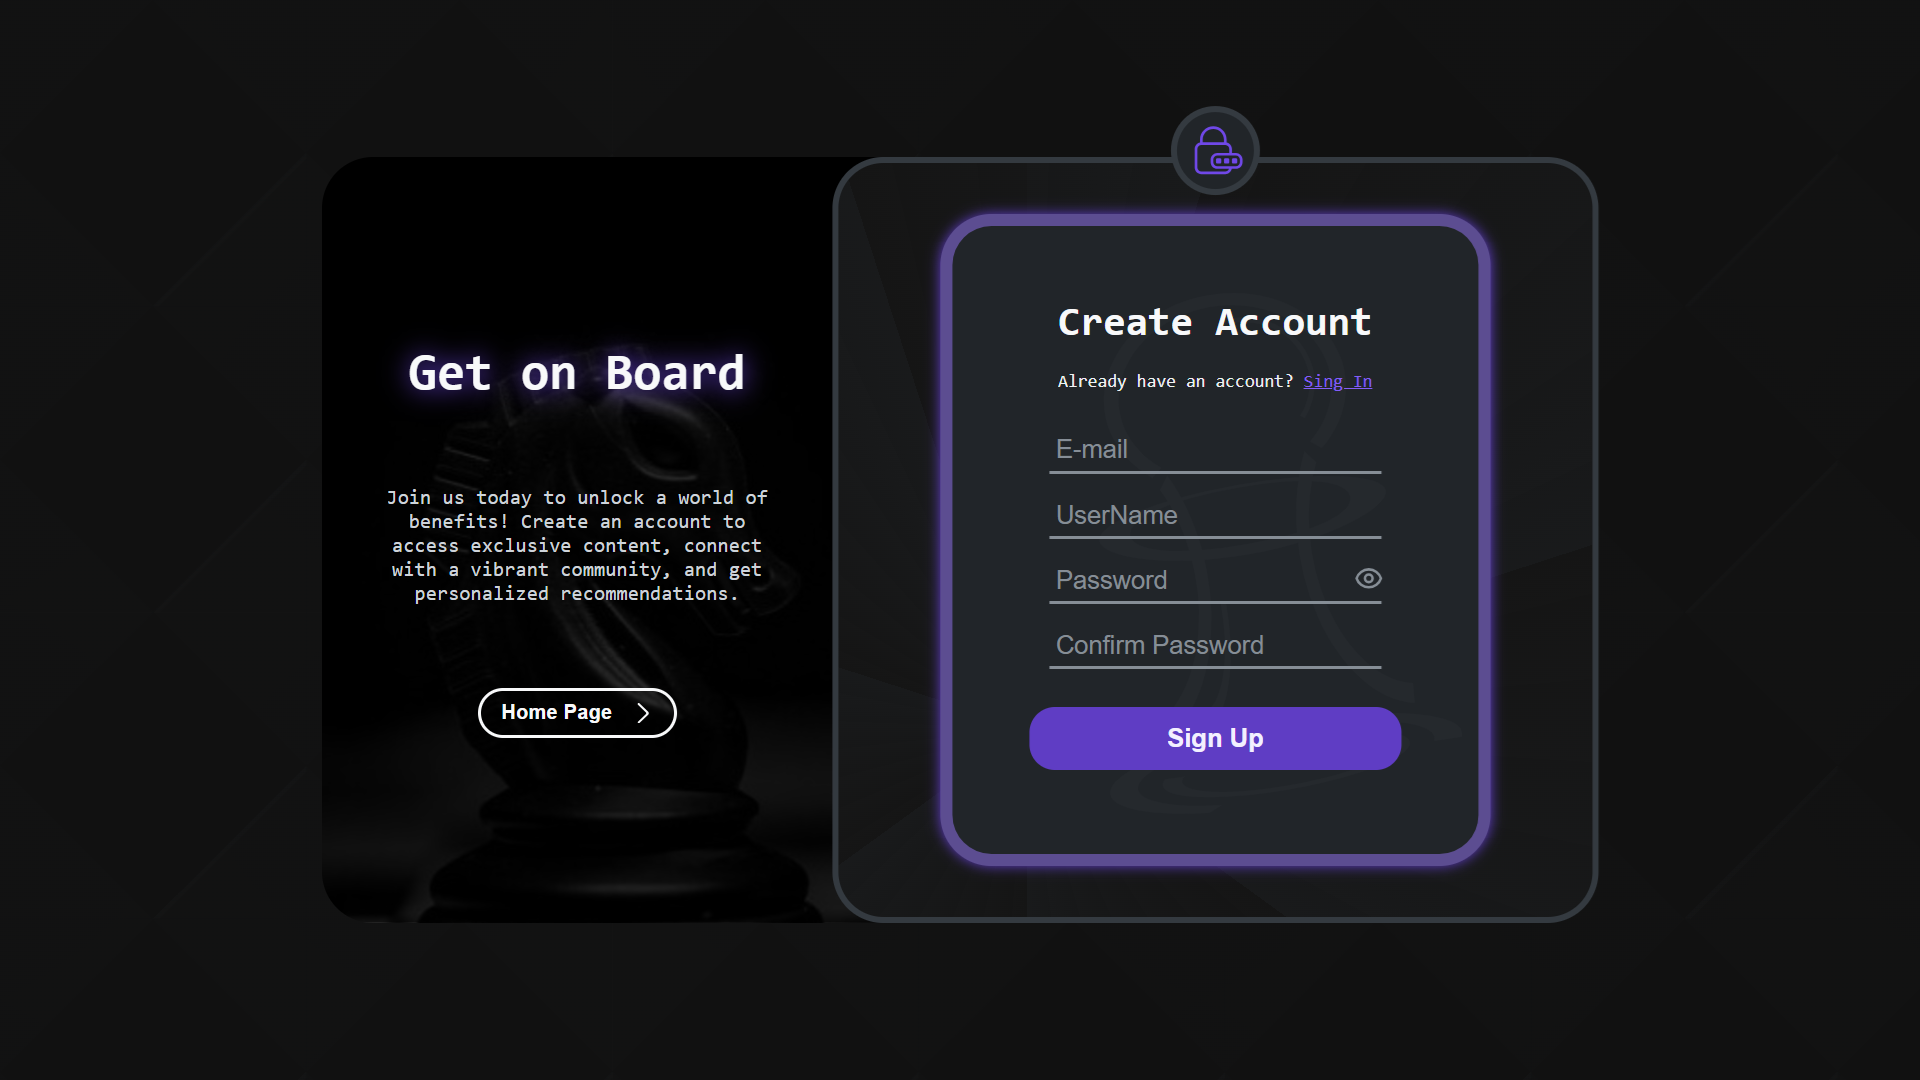
\includegraphics[width=1\textwidth]{zdj/ins_reg.png}
    \caption{Widok strony startowej.}
\end{figure}

Strona rejestracji jest zaprojektowana z myślą o czytelności i łatwości obsługi, dzięki czemu użytkownicy mogą bez przeszkód korzystać z jej funkcji niezależnie od poziomu zaawansowania. Wszystkie kroki są jasno opisane, a interfejs dostosowano do potrzeb zarówno nowych, jak i stałych użytkowników aplikacji.

\newpage
\subsection{Weryfikacja konta}

\begin{minipage}[t]{0.45\textwidth} 
    \vspace{0pt} 
    \raggedright 
    Weryfikacja konta to jeden z kluczowych etapów rejestracji, mający na celu zapewnienie bezpieczeństwa danych użytkowników oraz ochronę przed nieuprawnionym dostępem. Po zakończeniu procesu rejestracji aplikacja automatycznie generuje wiadomość e-mail, która zawiera wszystkie informacje niezbędne do ukończenia weryfikacji. System weryfikacyjny nie tylko wspiera proces zakładania konta, ale również jest wykorzystywany przy odzyskiwaniu hasła, co zapewnia spójność działania i zwiększa bezpieczeństwo użytkowników. 
\end{minipage} 
\hfill 
\begin{minipage}[t]{0.45\textwidth} 
    \vspace{0pt} 
    \centering 
    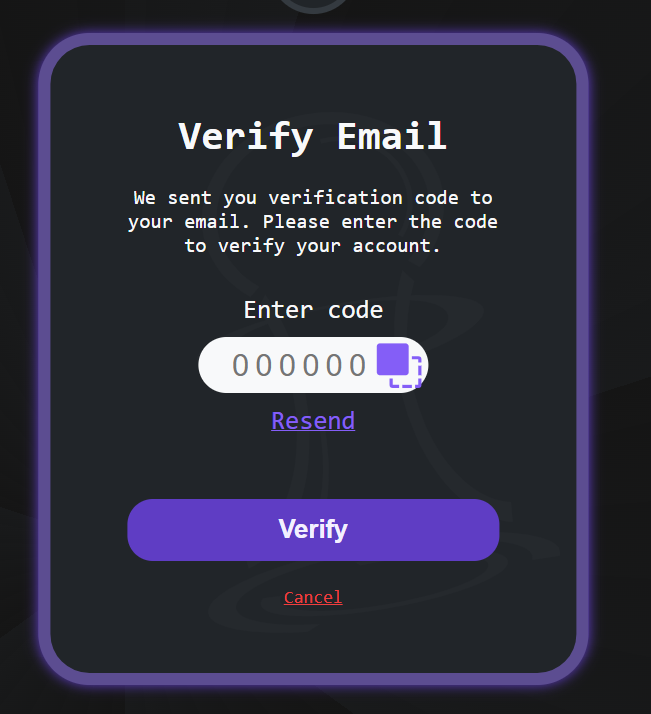
\includegraphics[width=\linewidth]{zdj/ins_min_ver.png} 
\end{minipage}
\vspace{1cm}
\begin{minipage}[t]{0.45\textwidth} 
    \vspace{0pt} 
    \centering 
    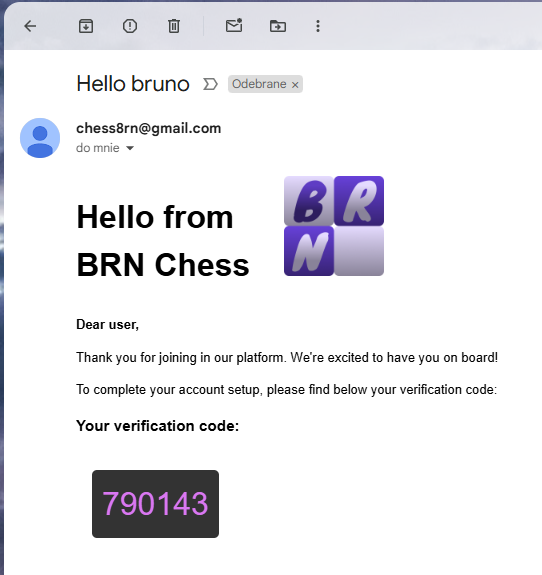
\includegraphics[width=\linewidth]{zdj/ins_min_mail.png} 
\end{minipage} 
\hfill 
\begin{minipage}[t]{0.45\textwidth} 
    \vspace{0pt} 
    \raggedright 
    Wiadomość e-mail, zatytułowana "Hello from BRN Chess", zawiera przyjazne powitanie, a także unikalny kod weryfikacyjny przypisany do konkretnego konta użytkownika. Treść e-maila została zaprojektowana tak, aby była czytelna i estetyczna, co pozwala na szybkie odnalezienie wymaganych informacji. Kod weryfikacyjny, przedstawiony w formie wyróżnionego tekstu, należy skopiować i wkleić w dedykowane pole tekstowe w oknie weryfikacji w aplikacji. Po wprowadzeniu kodu i jego zatwierdzeniu konto zostaje w pełni aktywowane, a użytkownik może rozpocząć korzystanie z platformy. 
\end{minipage}
\vspace{1cm}

Cały proces został opracowany z myślą o wygodzie użytkownika. Okno weryfikacyjne w aplikacji jest intuicyjne, zawiera czytelne instrukcje oraz widoczne przyciski umożliwiające wprowadzenie kodu. Dodatkowo w przypadku problemów, takich jak brak dostarczenia wiadomości e-mail, aplikacja oferuje możliwość ponownego wysłania kodu weryfikacyjnego za pomocą jednego kliknięcia.
\\\\
Weryfikacja konta to proces szybki i bezproblemowy, a dzięki jasnym instrukcjom użytkownicy mogą sprawnie zakończyć konfigurację swojego konta i skupić się na odkrywaniu możliwości aplikacji.

\newpage
\subsection{Strona główna}
Strona główna aplikacji szachowej została zaprojektowana z myślą o intuicyjnej nawigacji i szybkim dostępie do kluczowych funkcji, aby zapewnić użytkownikom wygodę i efektywność. Po prawej stronie ekranu znajduje się pasek nawigacji, który umożliwia łatwe przechodzenie między różnymi stronami aplikacji, zapewniając dostęp do wszystkich istotnych sekcji. Pasek został umieszczony w widocznym miejscu, dzięki czemu poruszanie się po aplikacji jest szybkie i płynne.
\\\\
Obok paska nawigacji umieszczono główne przyciski, które prowadzą do najważniejszych funkcji aplikacji. Każdy z nich odpowiada za inną czynność:
\begin{itemize}
    \item \textbf{Gra online:} umożliwia rozpoczęcie partii z innym graczem przez internet.
    \item \textbf{Gra z komputerem:} pozwala zmierzyć się z silnikiem szachowym.
    \item \textbf{Gra ze znajomymi:} umożliwia zapraszanie znajomych do wspólnej gry.
    \item \textbf{Wgląd w gry użytkownika:} pokazujące zakończone jak i wciąż trwające partie.
    \item \textbf{Zaproszenia do gier:} wyświetla listę otrzymanych zaproszeń do rozgrywek.
\end{itemize}

Pozostałą przestrzeń zajmują okna szybkiego dostępu, takie jak podgląd konta użytkownika, szybka gra online z wyborem trzech trybów czasowych (1 min, 3 min, 10 min), a także widok trzech ostatnich zakończonych i trzech aktywnych gier. Całość jest intuicyjna, zapewniając wygodne korzystanie z aplikacji.

\begin{figure}[h!]
    \centering
    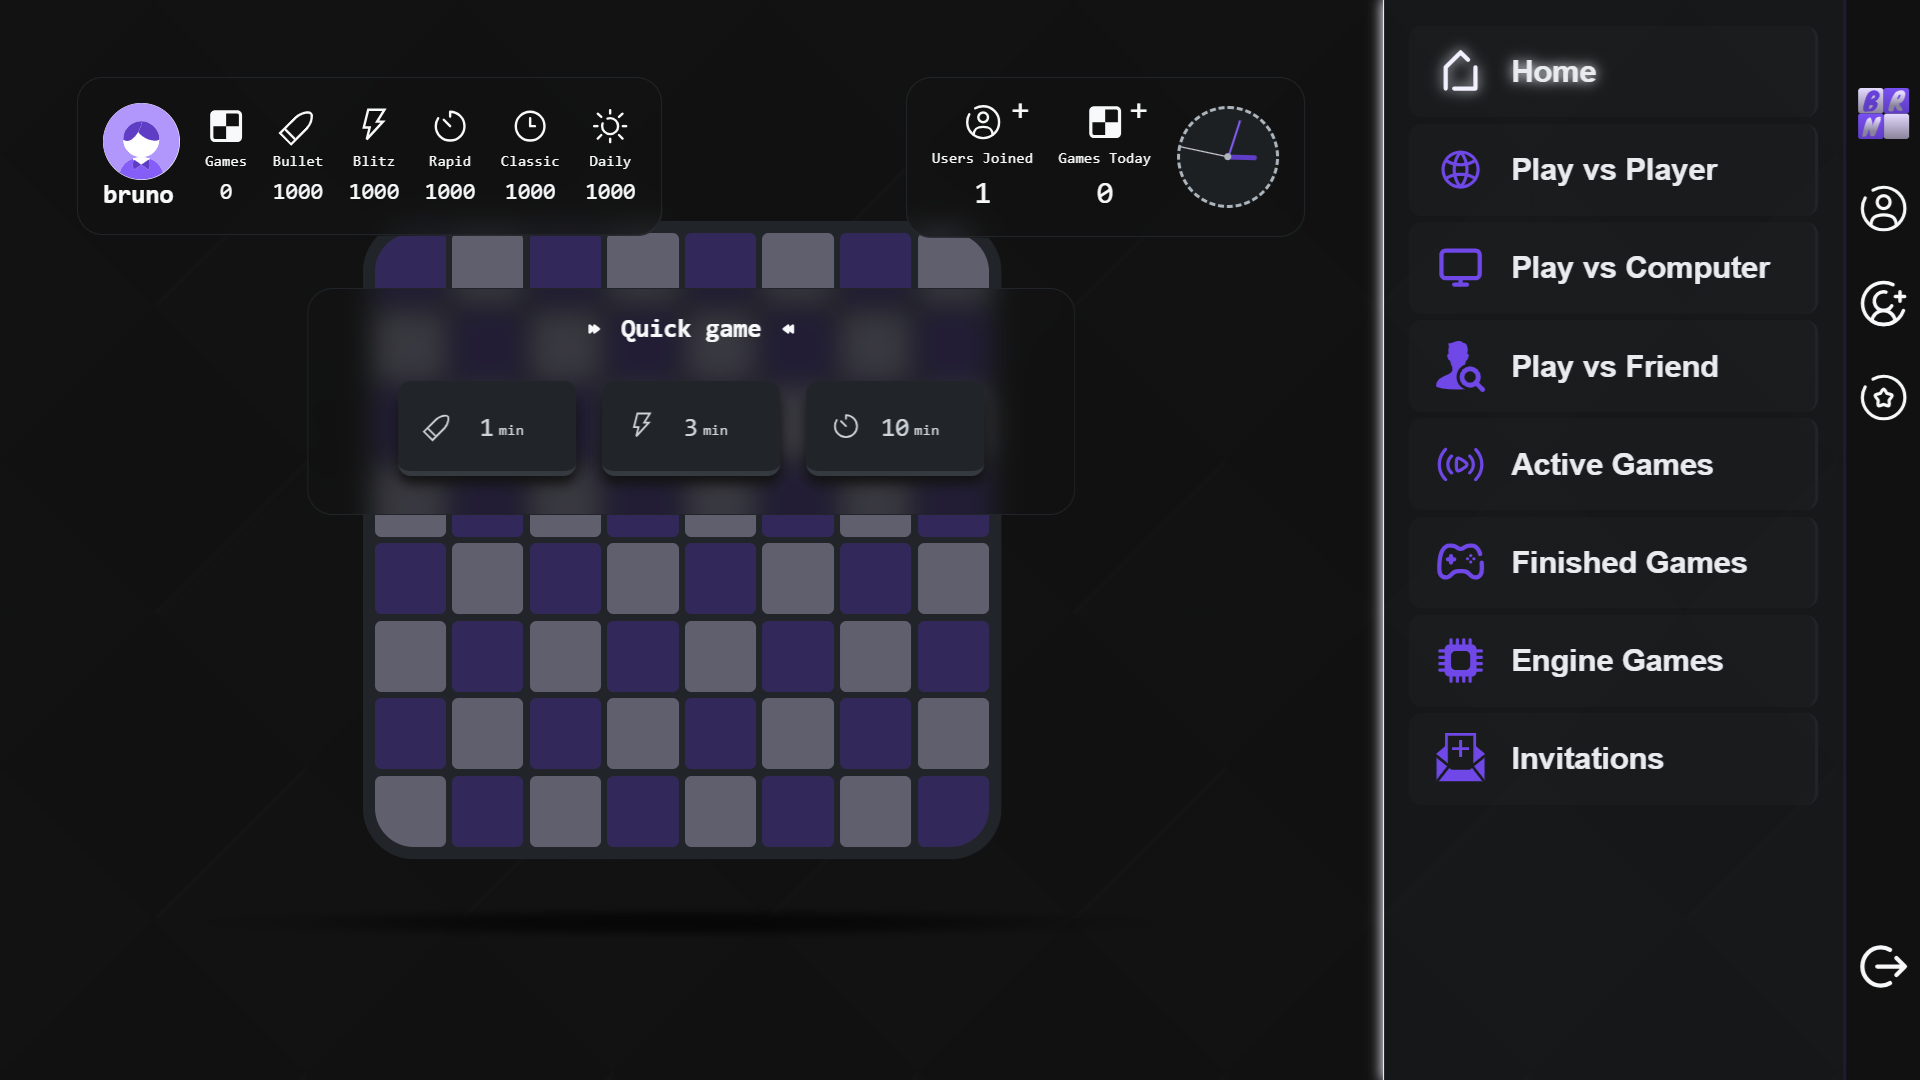
\includegraphics[width=1\textwidth]{zdj/ins_main.png}
    \caption{Widok strony głównej.}
\end{figure}

\newpage
\subsection{Gra online}
Po kliknięciu na przycisk gry online, użytkownik zostaje przeniesiony do okna, które pozwala na wybór odpowiedniego trybu kontroli czasowej dla gry. W zależności od preferencji, dostępne są różne opcje czasowe, zgrupowane w kategorie, takie jak bullet, blitz, rapid, classic oraz daily.
\\\\
W sekcji bullet użytkownik ma do wyboru bardzo szybkie tryby, takie jak 1 minuta bez dodatkowego czasu (1min), z dodatkowymi sekundami (1m|1s), lub 2 minuty z opcją 1 sekundy dodatkowego czasu (2m|1s). Dla blitz oferowane są opcje 3 minuty, 3 minuty z 5 sekundami dodatkowego czasu, 5 minut, oraz 5 minut z 10 sekundami dodatkowymi. W przypadku rapid dostępne są opcje 10 minut, 15 minut oraz 30 minut. Tryby classic pozwalają na bardzo długie partie z czasem od 1 godziny do 5 godzin, w zależności od preferencji gracza. Ostatnia kategoria, daily, oferuje najbardziej rozciągnięte w czasie partie, gdzie każdy gracz ma od 1 do 30 dni na rozegranie partii.
\\\\
Po dokonaniu wyboru jednego z powyższych trybów, ekran zmienia się na widok wyszukiwania przeciwnika. W tym momencie system zaczyna szukać dostępnego gracza o podobnym czasie reakcji, aby rozpocząć rozgrywkę. Użytkownik może na bieżąco śledzić postęp tego procesu, a po znalezieniu przeciwnika następuje połączenie i rozpoczęcie gry.

\begin{figure}[h!]
    \centering
    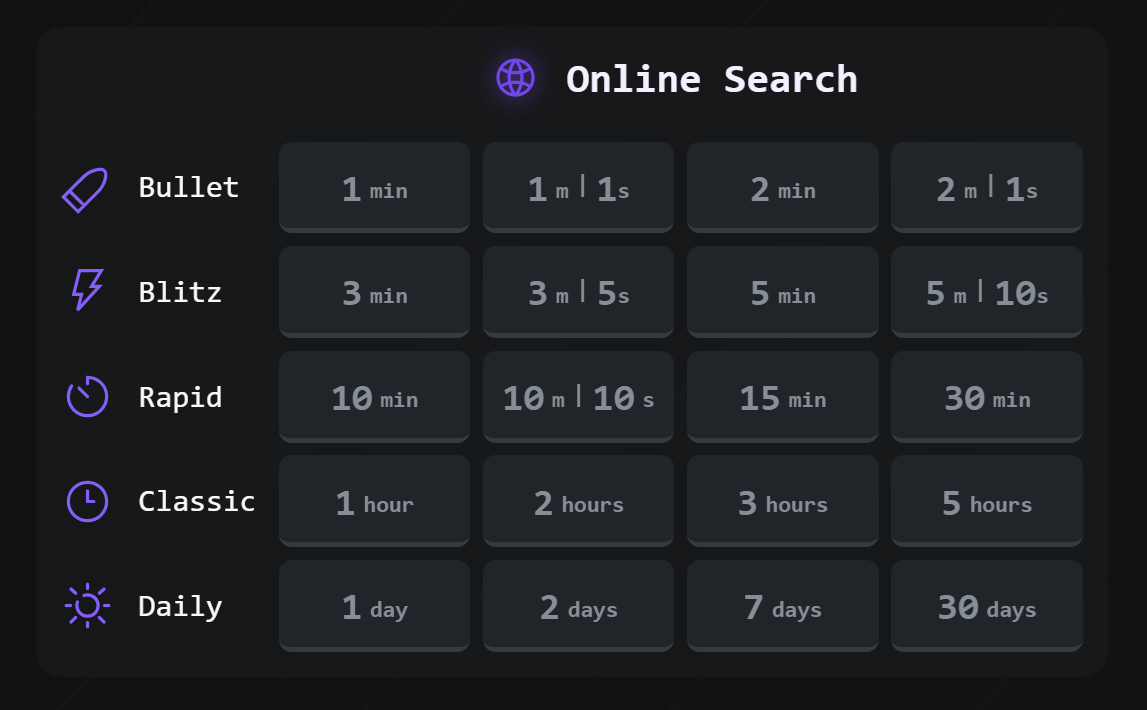
\includegraphics[width=1\textwidth]{zdj/ins_min_pvp.png}
    \caption{Widok wyboru gry online.}
\end{figure}

\newpage
\subsection{Gra offline}
Po kliknięciu na przycisk "Gra z komputerem", użytkownik zostaje poproszony o wybór poziomu trudności silnika. Istnieje 20 poziomów, które symbolicznie podzielono na cztery kategorie: standard, intermediate, advanced oraz master. Należy jednak podkreślić, że podział ten ma charakter jedynie orientacyjny i nie wpływa w żaden sposób na faktyczny sposób działania silnika. Jest to tylko sposób ułatwiający użytkownikowi poruszanie się po dostępnych opcjach, a wybór konkretnego poziomu zależy od indywidualnych preferencji gracza.
\\\\
Po dokonaniu wyboru poziomu silnika gra uruchamia się natychmiastowo, a użytkownik może zacząć rywalizować z komputerowym przeciwnikiem. Warto dodać, że w przypadku gry z komputerem nie ma zastosowanej kontroli czasowej, co oznacza, że gracz może spokojnie analizować ruchy bez presji czasu.
\\\\
Dodatkowo, podczas gry z komputerem istnieje opcja oszukiwania, czyli możliwość cofania ruchów lub zmiany poziomu silnika w trakcie rozgrywki. Ta funkcja daje graczowi elastyczność i pozwala na dostosowanie poziomu trudności w trakcie gry, jeśli uzna to za konieczne. Opcja ta jest jednak dostępna tylko w tej formie w grze z komputerem. Użytkownik może także zmienić preferencje dotyczące oszukiwania, a także inne ustawienia, na stronie swojego profilu, którą opisujemy w dalszej części instrukcji.

\begin{figure}[h!]
    \centering
    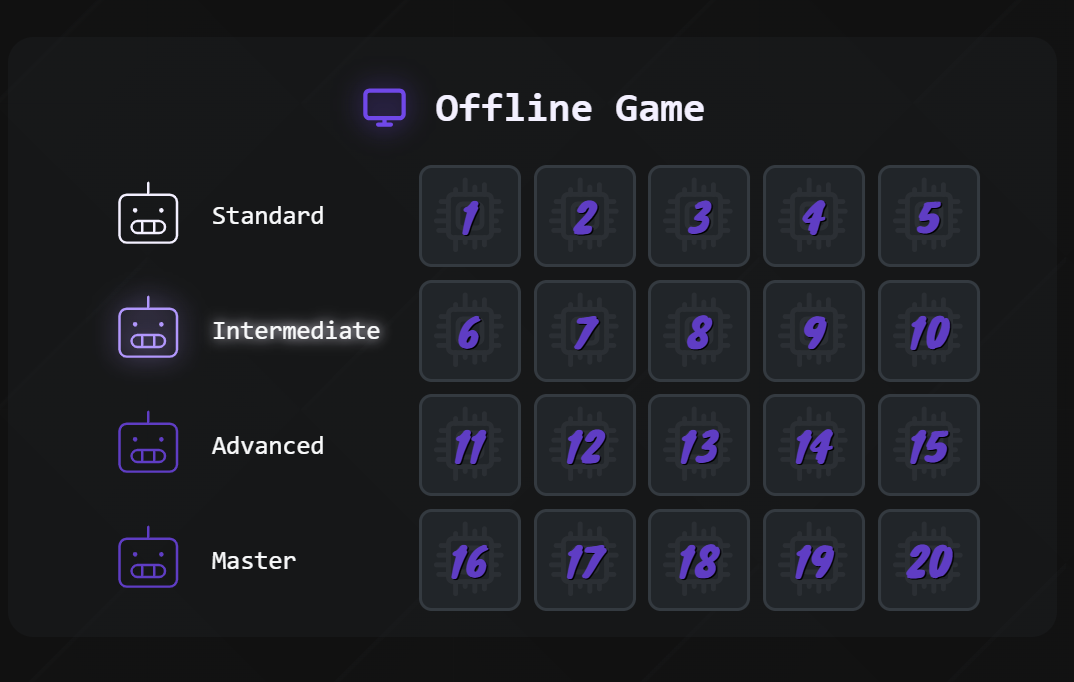
\includegraphics[width=1\textwidth]{zdj/ins_min_pvc.png}
    \caption{Widok wyboru gry offline.}
\end{figure}

\newpage
\subsection{Gra ze znajomymi}
Po kliknięciu na przycisk „Gra ze znajomymi”, użytkownik zostaje przeniesiony do okna, gdzie po lewej stronie znajduje się opcje zapraszania do gry, a po prawej widoczna jest lista wszystkich znajomych, którzy mają konto w aplikacji. Po kliknięciu na kartę znajomego użytkownik zostaje przekierowany do ekranu wyboru czasu gry, podobnie jak w przypadku gry online z losowym przeciwnikiem, gdzie wybiera się jedną z dostępnych opcji czasowych. Po dokonaniu wyboru czasu, gra natychmiast przechodzi do strony oczekiwania na dołączenie drugiego gracza, użytkownik będzie czekał, aż zaproszona osoba zaakceptuje zaproszenie i dołączy do gry.
\\\\

\begin{figure}[h!]
    \centering
    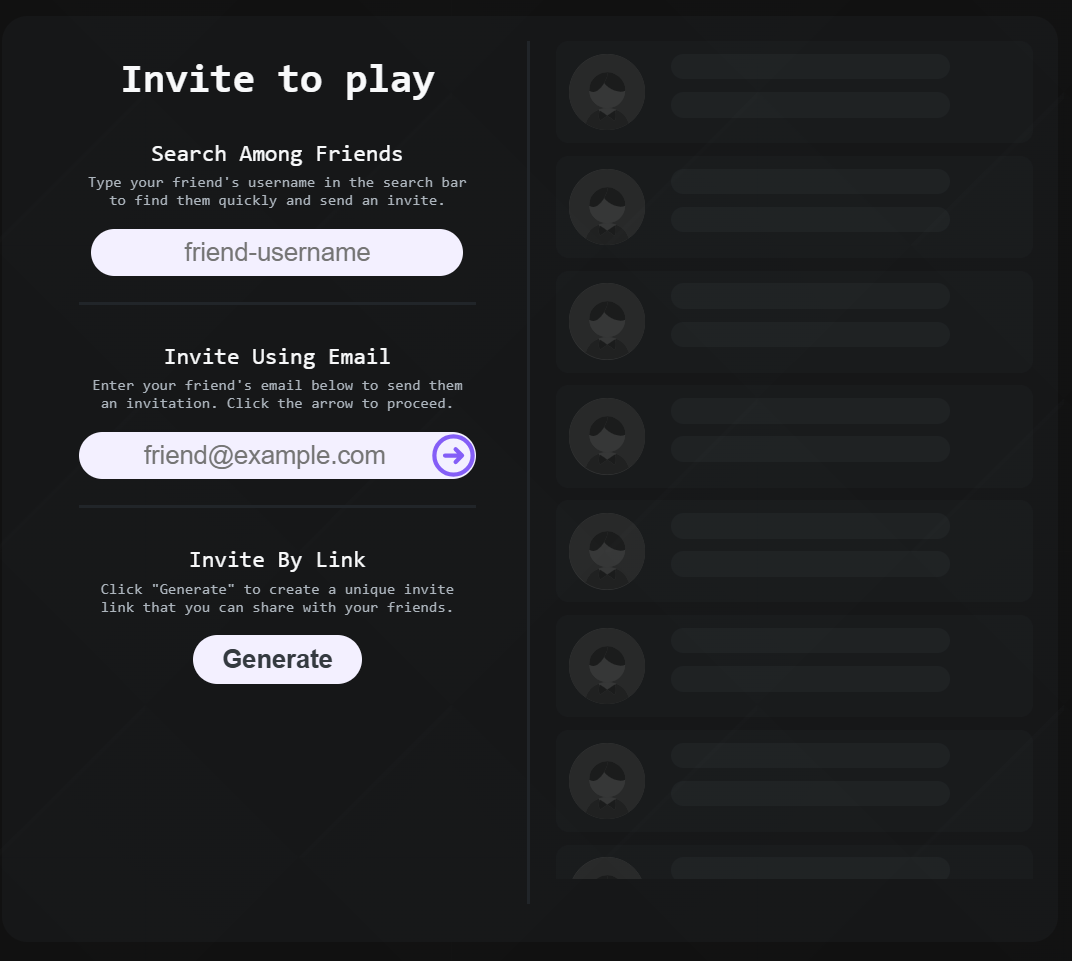
\includegraphics[width=1\textwidth]{zdj/ins_min_pvf.png}
    \caption{Widok wyboru gry ze znajomym.}
\end{figure}

\newpage
Po prawej stronie ekranu znajdują się trzy główne opcje umożliwiające zapraszanie do gry. Pierwsza z nich pozwala na filtrowanie znajomych po nazwie użytkownika. Dzięki temu, w przypadku długiej listy znajomych, łatwiej można znaleźć konkretnego gracza. Druga opcja to bezpośrednie zaproszenie przez e-mail. Po podaniu prawidłowego adresu e-mail użytkownik zostaje przekierowany do wyboru czasu gry, tak jak ma to miejsce w przypadku zapraszania znajomego z listy. Jeśli jednak wprowadzony adres e-mail jest niepoprawny lub nie istnieje w systemie, aplikacja wyświetli komunikat informujący, że taki użytkownik nie istnieje. Dzięki tej funkcji użytkownicy mogą zapraszać do gry nie tylko swoich znajomych, ale także osoby spoza listy znajomych, wystarczy, że podadzą poprawny adres e-mail. Jeśli podany adres jest prawidłowy i istnieje w systemie, zaproszenie zostaje wysłane, a użytkownik zostaje przekierowany do wyboru czasu gry.
\\\\
Trzecia opcja, „Gra za pomocą wygenerowanego linka”, pozwala na zaproszenie do gry gracza, który nie jest bezpośrednio na liście znajomych. Po dokonaniu wyboru kontroli czasowej, wyświetla się zmodyfikowane okno oczekiwania, w którym pojawi się unikalny link. Link ten jest kluczowy dla całej procedury – to za jego pomocą zapraszający gracz będzie mógł zaprosić innego użytkownika do dołączenia do gry. W celu rozpoczęcia gry, zapraszający użytkownik musi skopiować wygenerowany link i wysłać go znajomemu za pomocą dowolnego komunikatora, na przykład e-maila, messengera lub innej aplikacji. Po kliknięciu w link przez zaproszonego gracza, następuje przekierowanie na specjalną stronę, która automatycznie dołączy tego gracza do gry. Kiedy obaj gracze wejdą na tę stronę, będą przekierowani do samej gry, gdzie rozgrywka się rozpocznie. Jeśli jednak zapraszający kliknie w link, aby dołączyć do gry, otrzyma komunikat o błędzie, ponieważ nie może dołączyć do własnej gry. System wyświetli informację, że musi to być inny gracz, który kliknie w link, aby rozpocząć rozgrywkę. Dzięki temu proces zapraszania i dołączania do gry jest prosty, a użytkownik zapraszający ma pełną kontrolę nad wysłaniem linku do odpowiedniej osoby.

\begin{figure}[h!]
    \centering
    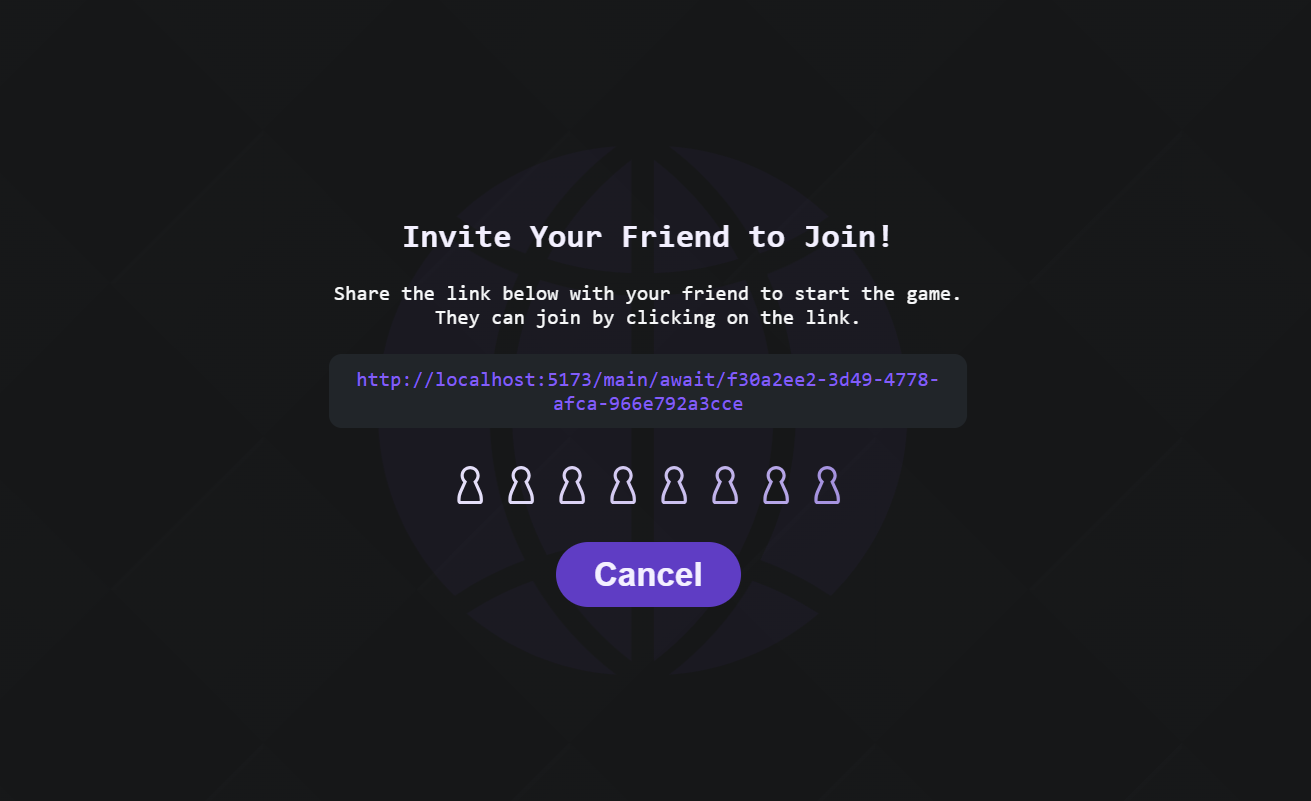
\includegraphics[width=1\textwidth]{zdj/ins_min_link.png}
    \caption{Widok rozpoczynania gry przez link.}
\end{figure}

\newpage
\subsection{Gry użytkownika}
Po kliknięciu na przyciski wyświetlające gry, użytkownik zostaje przeniesiony do sekcji, w której pojawiają się karty gier. W zależności od wybranego przycisku, wyświetlane są gry w różnych stanach. W sekcji „Wciąż aktywne gry” znajdują się partie, które są w trakcie rozgrywki. Jest to szczególnie użyteczne przy długich czasach gry, gdyż gracze mogą wrócić do nierozgrywanych jeszcze partii, kontynuując je w dowolnym momencie. Sekcja „Zakończone gry” pozwala na przeglądanie gier, które już się zakończyły. Użytkownicy mogą sprawdzić, jak przebiegały rozgrywki, jakie strategie były stosowane i jakie były wyniki. Sekcja „Gry z komputerem” oferuje podobną funkcjonalność, umożliwiając przegląd zakończonych gier przeciwko komputerowemu przeciwnikowi. Dzięki temu gracze mogą łatwo wrócić do swoich partii, analizować je i śledzić postępy w grze. Aby powrocic do gry, użytkownik musi zwyczajnie kliknąć w wybraną kartę.
\\\\
Dodatkowo, we wszystkich tych sekcjach istnieją filtry, które umożliwiają łatwiejsze sortowanie gier. Gracze mogą filtrować partie po różnych kryteriach, takich jak rodzaj kontroli czasowej, co pozwala szybko znaleźć gry o określonym czasie, czy wynik gry, umożliwiając sortowanie na podstawie zwycięstw, porażek lub remisów. Filtry te ułatwiają przeglądanie dużej liczby gier, pomagając użytkownikom szybko odnaleźć interesujące ich rozgrywki i dostosować widok do swoich potrzeb.

\begin{figure}[h!]
    \centering
    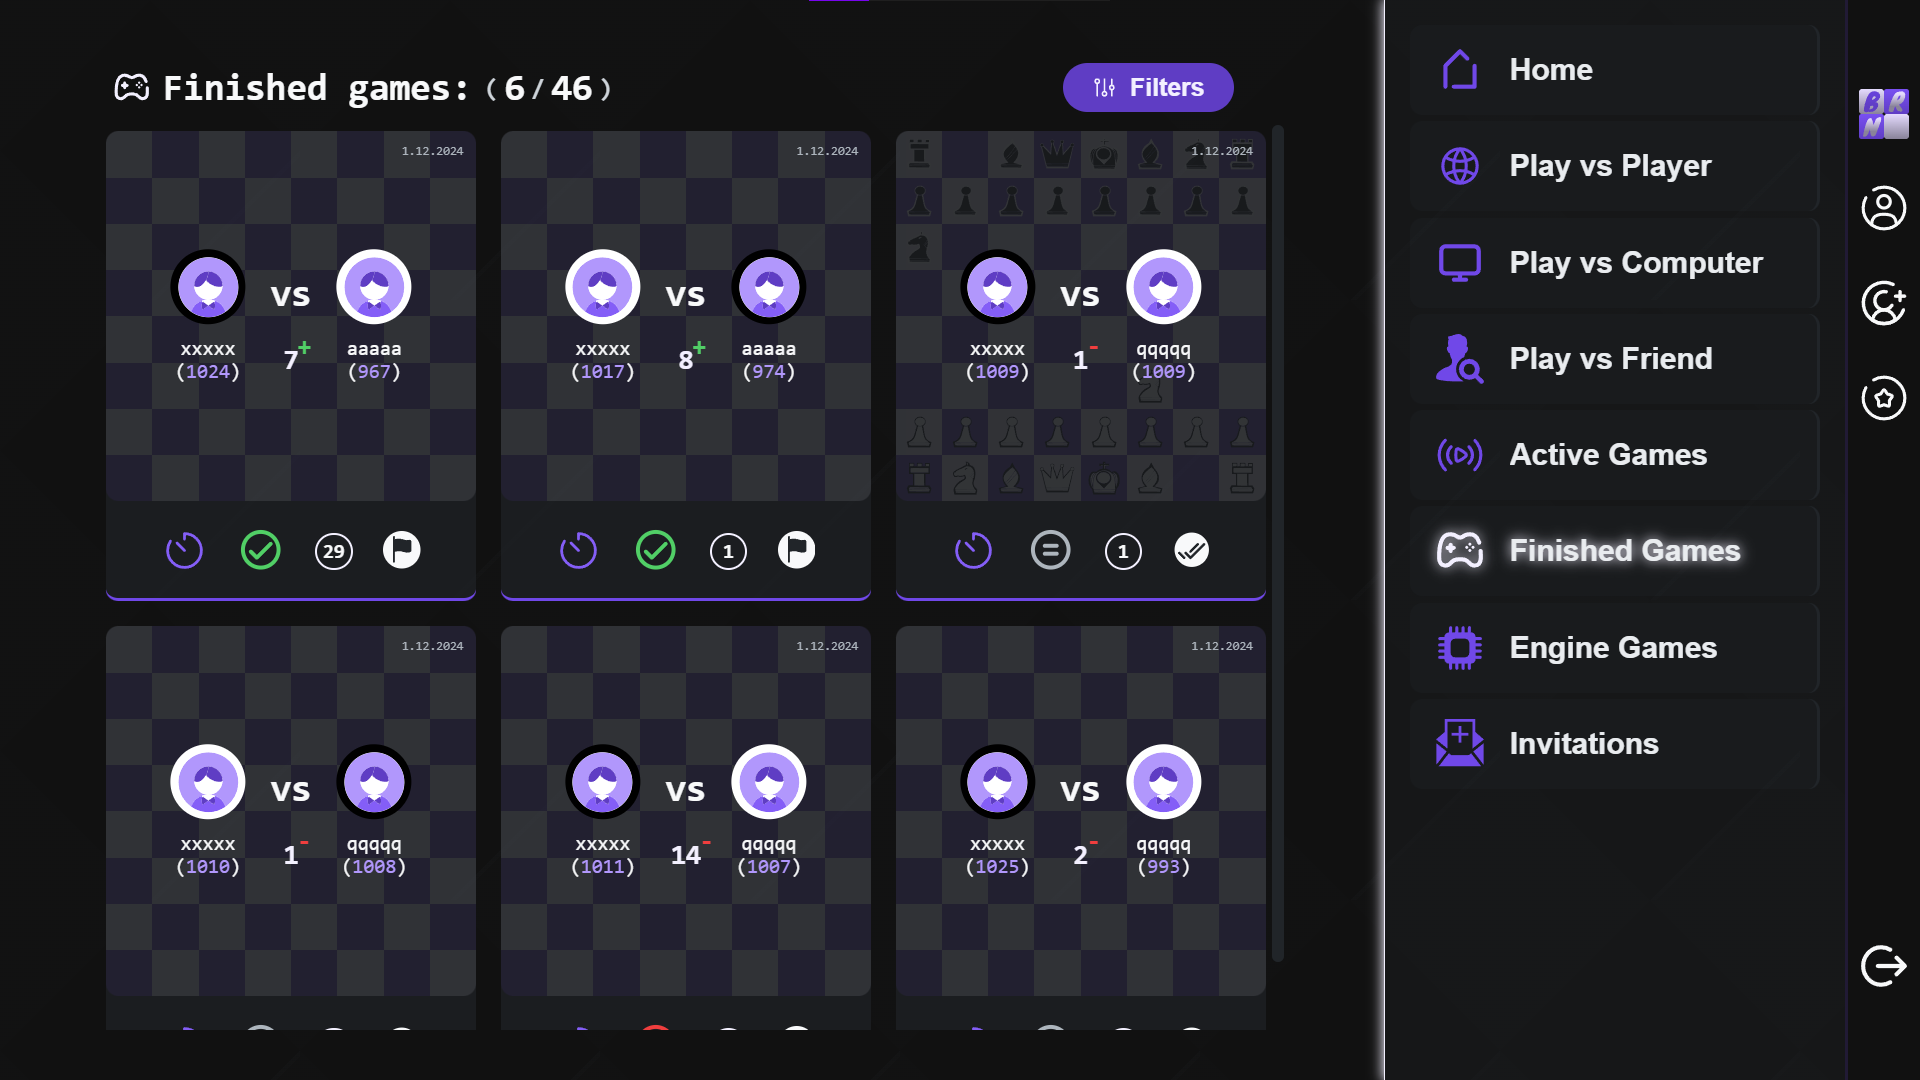
\includegraphics[width=1\textwidth]{zdj/ins_min_games.png}
    \caption{Widok gier użytkownika.}
\end{figure}

\newpage
\subsection{Zaproszenia}
Ostatnia sekcja na głównej stronie to zaproszenia, gdzie użytkownik ma wgląd we wszystkie aktywne zaproszenia do gry. Zaproszenia te mają określony czas ważności – wygasają po 15 minutach, po czym przestają być widoczne. Dzięki temu użytkownicy mają tylko ograniczony czas na przyjęcie zaproszenia, co wprowadza element dynamiki i pilności w interakcje z innymi graczami.

\begin{figure}[h!]
    \centering
    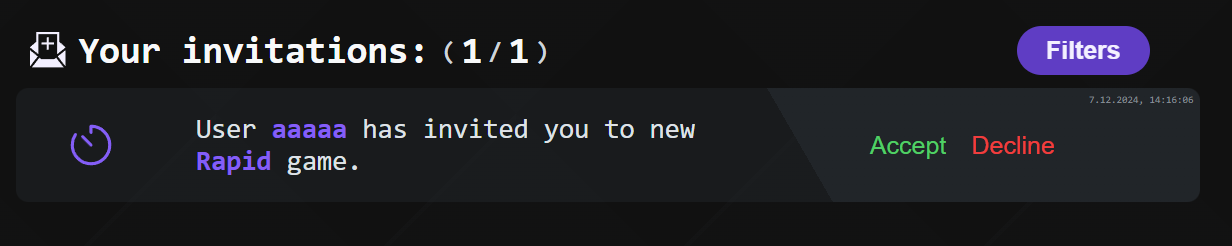
\includegraphics[width=1\textwidth]{zdj/ins_min_inv_card.png}
    \caption{Widok zaproszeń do gry.}
\end{figure}

Dodatkowo, w przypadku gdy użytkownik jest aktywny na stronie, pojawia się specjalnie dedykowane okno popup. Jeśli użytkownik otrzyma zaproszenie do gry, komunikat wyświetli się automatycznie, informując o tym fakcie. W popupie znajdują się również opcje akceptacji lub odrzucenia zaproszenia, co umożliwia szybkie podjęcie decyzji o dołączeniu do gry lub jej odrzuceniu. Dzięki tej funkcji użytkownicy są na bieżąco informowani o zaproszeniach, co ułatwia interakcję i organizowanie rozgrywek. Użytkownik także może użyć filtrów, aby wyświetli już nieaktywne zaproszenia.

\begin{figure}[h!]
    \centering
    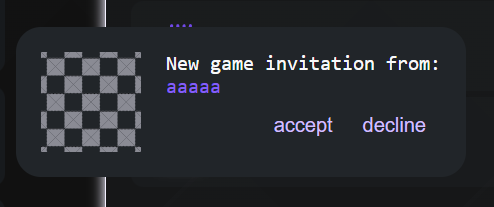
\includegraphics[width=0.7\textwidth]{zdj/ins_min_inv_popup.png}
    \caption{Wyskakujące okienko otrzymanego zaproszenia.}
\end{figure}

\newpage
\subsection{Strona gry}
Na stronie gry, w centralnej części, znajduje się szachownica, która stanowi główny element interfejsu. To tutaj odbywa się sama rozgrywka, a użytkownicy wykonują swoje ruchy. Po obu stronach szachownicy znajdują się panele, które oferują dodatkowe opcje i funkcjonalności, zapewniając pełniejszą kontrolę nad grą i umożliwiając dostęp do różnych narzędzi pomocniczych.

\begin{figure}[h!]
    \centering
    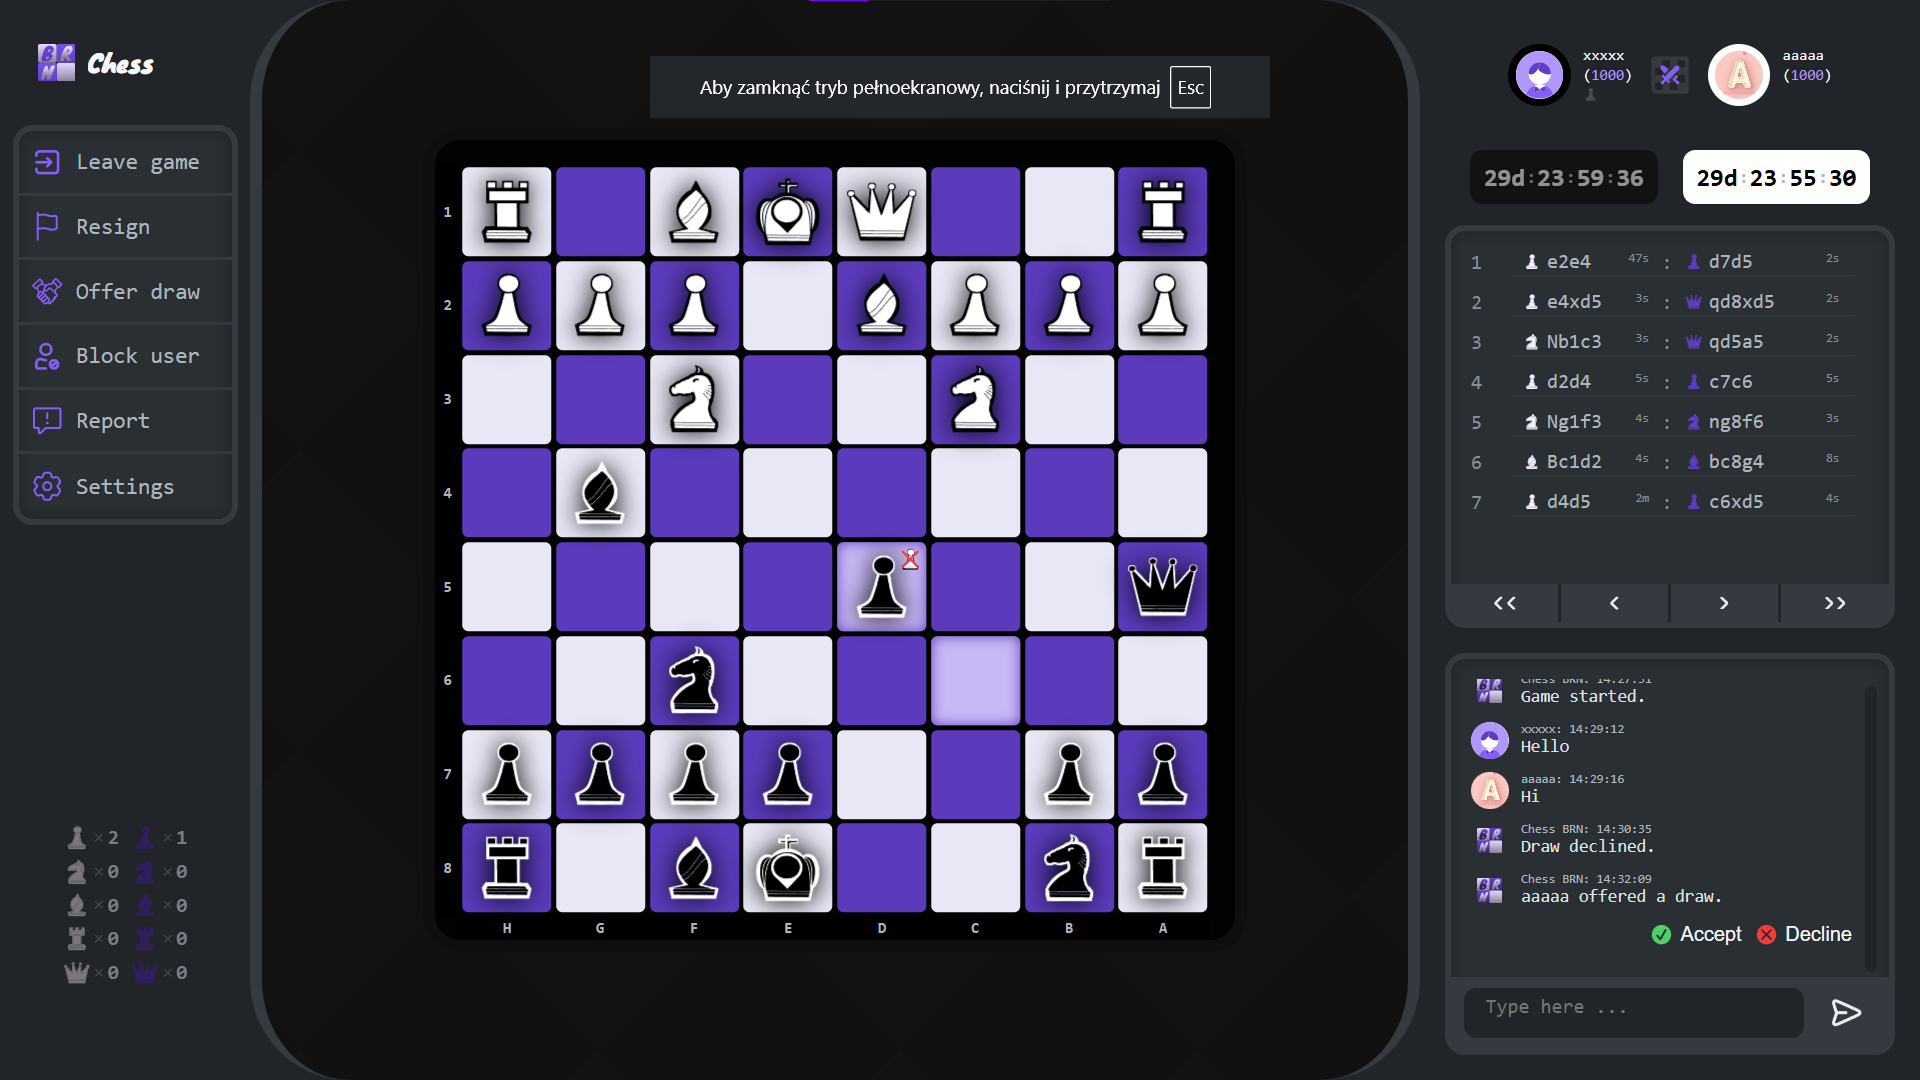
\includegraphics[width=0.9\textwidth]{zdj/ins_webgame.png}
    \caption{Strona gry online.}
\end{figure}

\begin{figure}[h!]
    \centering
    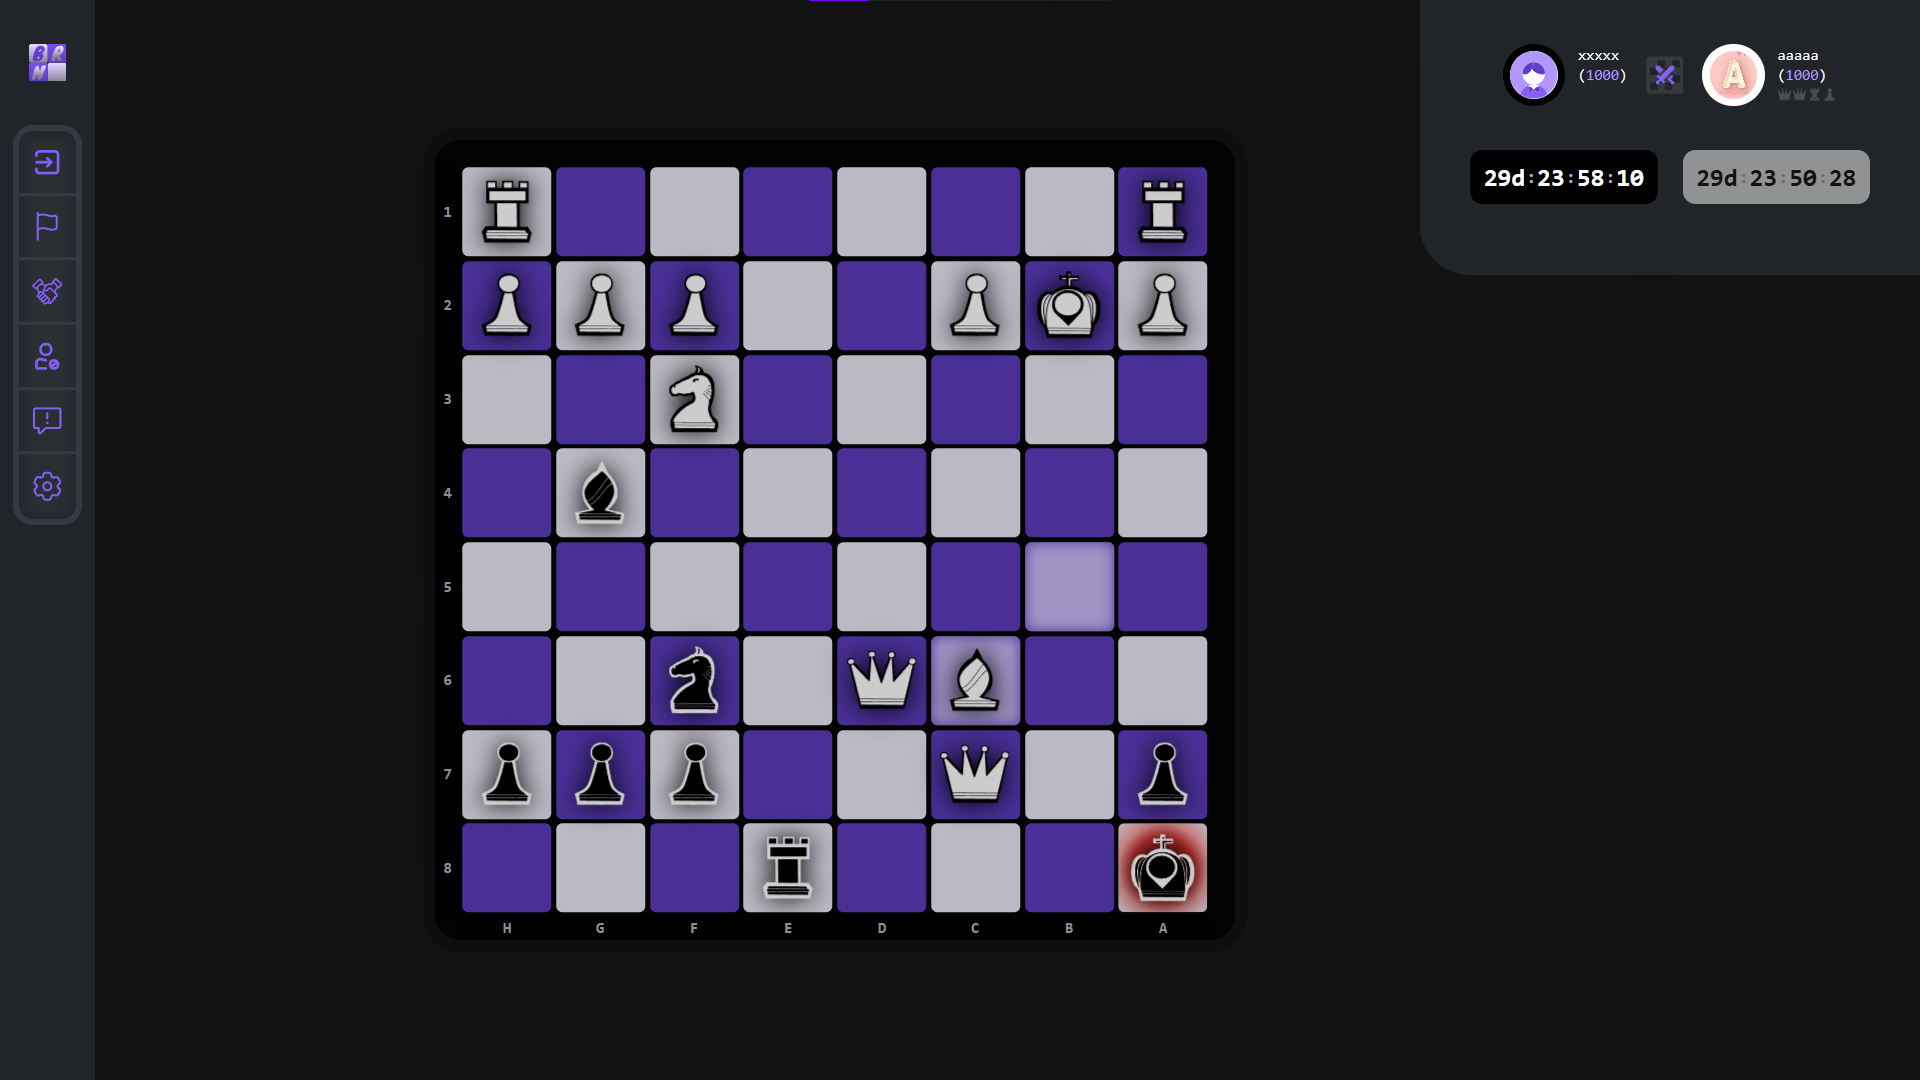
\includegraphics[width=0.9\textwidth]{zdj/ins_simpgame.png}
    \caption{Uproszony widok gry.}
\end{figure}

\newpage

W centralnej części ekranu znajduje się szachownica, której wygląd może być spersonalizowany przez użytkownika w ustawieniach. Po bokach planszy wyświetlane są koordynaty pól (oznaczone literami i cyframi), które pomagają w orientacji na szachownicy. Gracze mogą wybierać i wykonywać ruchy zarówno poprzez kliknięcia, jak i metodę drag and drop, przeciągając figury na odpowiednie pola. Po wykonaniu ruchu przez przeciwnika, odpowiednie pole zostaje podświetlone, co ułatwia śledzenie zmian na planszy. W przypadku zbicia figury, na polu, na którym nastąpiło zbicie, pojawia się mała przekreślona ikona, sygnalizująca utratę figury. Gdy król znajduje się w szachu, jego figura zostaje podświetlona na czerwono, co wskazuje na zagrożenie i konieczność podjęcia działań w celu ochrony króla.

\begin{figure}[h!]
    \centering
    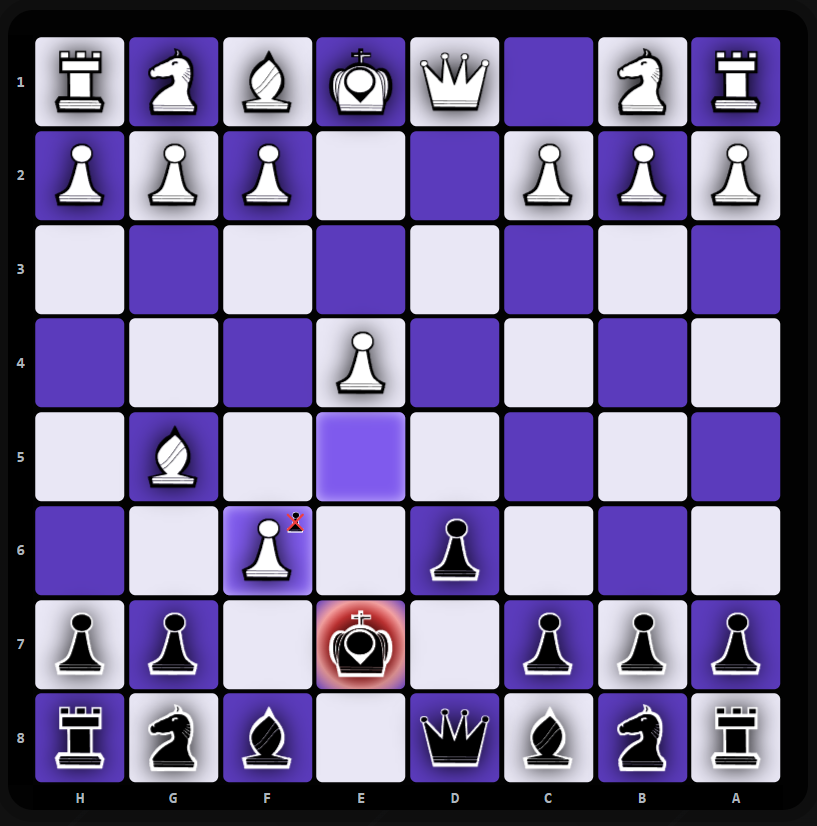
\includegraphics[width=0.9\textwidth]{zdj/ins_min_board.png}
    \caption{Szachownica}
\end{figure}

\newpage

\begin{minipage}[t]{0.45\textwidth} 
    \vspace{0pt} 
    \raggedright 
    Na prawym pasku widnieje informacja o graczach. Pokazuje ich aktualną punktację ELO oraz przewagę materialną w grze, przeliczoną na figury. Dodatkow zaraz poniżej znajduję się czas jaki pozostał każdemu z graczy, istniejący tylko w grach online (nie istnieje podczas gier z silnikiem).
\end{minipage} 
\hfill 
\begin{minipage}[t]{0.45\textwidth} 
    \vspace{0pt} 
    \centering 
    \includegraphics[width=\linewidth]{zdj/ins_min_players.png} 
\end{minipage}
\vspace{1cm}
\begin{minipage}[t]{0.45\textwidth} 
    \vspace{0pt} 
    \centering 
    \includegraphics[width=\linewidth]{zdj/ins_min_moves.png} 
\end{minipage} 
\hfill 
\begin{minipage}[t]{0.45\textwidth} 
    \vspace{0pt} 
    \raggedright 
    Kolejna funkcjonalność to menu ruchów, które zostały wykonane. Każdy ruch jest pokazany z ikoną figury, która została użyta, notacją FEN opisującą ruch oraz przybliżonym czasem wykonania ruchu. Na dole menu znajdują się strzałki umożliwiające przewijanie i cofanie, co pozwala na szybki podgląd poprzednich pozycji i śledzenie przebiegu partii. Dodatkowo, najeżdżając na konkretny ruch, wyświetla się wizualizacja pozycji po wykonaniu tego ruchu. Po zakończeniu partii pojawia się przycisk umożliwiający animację całej gry, pozwalając na jej odtworzenie od początku do końca.
\end{minipage}
\vspace{1cm}
\begin{minipage}[t]{0.45\textwidth} 
    \vspace{0pt} 
    \raggedright 
    Ostatnia funkcjonalność na prawym pasku to menu wiadomości. Wyświetlane są tam wiadomości wysłane przez użytkowników, jak również automatyczne powiadomienia, takie jak informacje o rozpoczęciu/zakończeniu gry czy oferta remisu. Na dole menu znajduje się pole do wysyłania własnych wiadomości, co umożliwia graczom łatwą komunikację z innymi uczestnikami gry. W przypadku gry z silnikiem wysłanie wiadomosci jest zablokowane, a wyswietlane sa tylko wiadomosci systemowe.
\end{minipage} 
\hfill 
\begin{minipage}[t]{0.45\textwidth} 
    \vspace{0pt} 
    \centering 
    \includegraphics[width=\linewidth]{zdj/ins_min_mess.png} 
\end{minipage}

\newpage

\begin{minipage}[t]{0.2\textwidth} 
    \vspace{0pt} 
    \centering 
    \includegraphics[width=\linewidth]{zdj/ins_min_wopt.png} 
\end{minipage} 
\hfill 
\begin{minipage}[t]{0.7\textwidth} 
    \vspace{0pt} 
    \raggedright 
    Na lewym panelu w przypadku gry online dostępne są opcje zarządzania rozgrywką. Pierwsza z nich to opcja opuszczenia gry, która działa różnie w zależności od długości partii. Dla gier krótkich oznacza to remis, jeśli gra dopiero się rozpoczęła, lub poddanie się, jeśli gra trwa już dłużej. W przypadku gier długich, opuszczenie gry oznacza po prostu wyjście z partii. Kolejna opcja to poddanie się, które kończy grę i uznaje przeciwnika za zwycięzcę. Można również zaproponować remis, co skutkuje wysłaniem oferty do drugiego gracza, który może ją zaakceptować lub odrzucić. Dodatkowo, istnieje opcja blokowania użytkownika, co uniemożliwia wysyłanie wiadomości oraz dodanie takiej osoby do znajomych. Istnieje również możliwość zgłoszenia podejrzenia oszukiwania, co daje użytkownikom narzędzie do zgłaszania nieuczciwych praktyk. Na koniec, dostępne jest ustawienie wyglądu strony gry, w tym zmiana wyglądu szachownicy oraz figur, co pozwala na dostosowanie interfejsu do własnych preferencji.
\end{minipage}
\vspace{1cm}
\begin{minipage}[t]{0.7\textwidth} 
    \vspace{0pt} 
    \raggedright 
    W przypadku gry z silnikiem, lewy panel zawiera nieco inne opcje dostosowane do tego trybu gry. Pierwsza opcja to wyjście z gry, która kończy rozgrywkę. Można również zrestartować grę, co rozpoczyna ją od nowa. Dodatkowo dostępna jest opcja poddania się, kończąca partię na korzyść silnika. Istnieje także możliwość cofnięcia ruchu, ale jest to dostępne tylko wtedy, gdy opcja oszukiwania jest włączona w ustawieniach. Kolejną opcją jest zmiana poziomu silnika, która pozwala na dostosowanie trudności rozgrywki, jednak ta funkcja jest także dostępna tylko przy włączonej opcji oszukiwania. Na koniec, jak w przypadku gry online, dostępna jest opcja zmiany ustawień wyglądu strony gry, w tym szachownicy oraz figur, co pozwala na personalizację wizualną rozgrywki.
\end{minipage} 
\hfill 
\begin{minipage}[t]{0.2\textwidth} 
    \vspace{0pt} 
    \centering 
    \includegraphics[width=\linewidth]{zdj/ins_min_eopt.png} 
\end{minipage}
\vspace{1cm}
\begin{minipage}[t]{0.2\textwidth} 
    \vspace{0pt} 
    \centering 
    \includegraphics[width=\linewidth]{zdj/ins_min_capt.png} 
\end{minipage} 
\hfill 
\begin{minipage}[t]{0.7\textwidth} 
    \vspace{0pt} 
    \raggedright 
    Ostatnią opcją na lewym panelu jest wyświetlanie zbitych figur. W tej sekcji widoczne są wszystkie figury, które zostały już zbite przez graczy, a obok każdej figury wyświetlana jest liczba, ile ich pozostało. Dzięki temu użytkownicy mogą śledzić, jak przebiega gra pod względem materiału, co pomaga w ocenie pozycji na szachownicy.
\end{minipage}

\newpage

Dodatkowo na planszy szachowej pojawiają się wyskakujące okna, które aktywują się po wybraniu odpowiednich opcji przez użytkownika. Takie okna zwykle służą do potwierdzenia wykonania konkretnej akcji, na przykład w przypadku chęci poddania się, opuszczenia gry czy zmiany ustawień. Wyskakujące okno zawiera pytanie, czy użytkownik na pewno chce wykonać daną czynność, a także opcje potwierdzenia lub anulowania decyzji. Dzięki temu gracze mają pewność, że nie dokonają niezamierzonych zmian czy działań.

\begin{minipage}[t]{0.45\textwidth} 
    \vspace{0pt} 
    \centering 
    Okno promocji pionka pojawia się, gdy pionek dotrze do ostatniej linii. Użytkownik wybiera jedną z czterech opcji: damę, wieżę, skoczka lub gońca, a pionek zostaje zamieniony na wybraną figurę.
\end{minipage} 
\hfill 
\begin{minipage}[t]{0.45\textwidth} 
    \vspace{0pt} 
    \centering 
    \includegraphics[width=\linewidth]{zdj/ins_min_prom.png} 
\end{minipage}
\vspace{1cm}
\begin{minipage}[t]{0.45\textwidth} 
    \vspace{0pt} 
    \centering 
    \includegraphics[width=\linewidth]{zdj/ins_min_prev.png} 
\end{minipage} 
\hfill 
\begin{minipage}[t]{0.45\textwidth} 
    \vspace{40pt}
    \centering 
    Pokazywanie poprzednich ruchów odbywa się po najechaniu myszką na menu z poprzednimi ruchami. Po wybraniu ruchu, na szachownicy pojawia się pomniejsza, przyciemniona plansza, która pokazuje wcześniejszą pozycję. Ta zmiana jest tylko wizualna, nie można nic zrobić na tej pomniejszonej planszy, służy ona jedynie do pokazania poprzedniego stanu gry.
\end{minipage}

\vspace{1cm}

\begin{minipage}[t]{0.45\textwidth} 
    \vspace{0pt} 
    \centering 
    Innym wyskakującym oknem jest okno, które pojawia się po zakończeniu gry, niezależnie od wyniku — wygranej, przegranej lub remisie. Na tym oknie wyświetlany jest rezultat gry, czyli informacja, kto wygrał, jaki był powód zakończenia gry oraz punkty zdobyte lub stracone przez graczy. Na dole okna znajdują się przyciski umożliwiające przejście do wyjścia z gry, rozpoczęcia nowej partii lub rozegrania rewanżu, przy czym będą one odbywać z dotychczasową kontrolą czasową. W przypadku gier z silnikiem dostępne są jedynie opcje restartu gry lub wyjścia z gry.
\end{minipage} 
\hfill 
\begin{minipage}[t]{0.45\textwidth} 
    \vspace{0pt} 
    \centering 
    \includegraphics[width=\linewidth]{zdj/ins_min_win.png} 
\end{minipage}

\newpage
\subsection{Strona profilu}
Strona profilu użytkownika zapewnia pełną kontrolę nad ustawieniami konta oraz personalizacją preferencji. Użytkownik ma możliwość edytowania swojego profilu, w tym zmiany danych osobowych, zdjęcia profilowego oraz innych informacji. Na stronie dostępne są szczegółowe statystyki gier, w tym wykresy punktacji dla różnych kategorii czasowych, które pozwalają na analizowanie postępów i wyników w różnych wariantach gier. Użytkownik może również przeglądać listę swoich znajomych, zapraszać ich do gry oraz oglądać ich profile.
\\\\
Dodatkowo, użytkownik ma możliwość edytowania ustawień konta, w tym zmiany hasła oraz zarządzania ustawieniami prywatności, takimi jak widoczność profilu. Można również dostosować wygląd strony gry, zmieniając szachownicę, pionki oraz inne elementy wizualne. Istnieje opcja włączenia funkcji oszukiwania podczas gry z silnikiem, co pozwala na cofanie ruchów lub zmianę poziomu trudności. Ponadto, użytkownik może zarządzać globalnymi ustawieniami aplikacji, takimi jak język czy powiadomienia. Strona profilu jest centralnym miejscem, w którym użytkownik może zarządzać wszystkimi aspektami swojego konta i dostosować aplikację do swoich potrzeb.

\begin{figure}[h!]
    \centering
    \includegraphics[width=1\textwidth]{zdj/ins_account.png}
    \caption{Strona profilu użytkownika.}
\end{figure}

\newpage
\subsection{Strona zarządzania znajomymi}
Strona użytkowników służy do zarządzania znajomymi i relacjami z innymi graczami w aplikacji. Jest podzielona na cztery główne sekcje, które pomagają w organizowaniu kontaktów.

\begin{itemize}
    \item \textbf{Wszyscy użytkownicy} – zawiera listę wszystkich graczy dostępnych w aplikacji. Z tej sekcji użytkownicy mogą zapraszać innych do znajomych oraz podglądać ich mini profile.
    \item \textbf{Twoi znajomi} – znajdują się tutaj osoby, które zostały już dodane do listy znajomych. Można stąd zapraszać znajomych do gry lub przejść do pełnego profilu danego użytkownika.
    \item \textbf{Oczekujące zaproszenia} – sekcja zawiera zaproszenia, które zostały wysłane, ale jeszcze nie zostały zaakceptowane przez drugą stronę. Użytkownicy mogą tu zobaczyć zarówno wysłane zaproszenia, jak i te, które czekają na odpowiedź.
    \item \textbf{Odrzucone zaproszenia} – lista osób, które odrzuciły zaproszenia do znajomych. Użytkownicy mają możliwość ponownego wysłania zaproszenia do tych osób, jeżeli zechcą.
\end{itemize}

Cała strona umożliwia łatwe zarządzanie znajomymi, zaproszeniami i relacjami z innymi graczami, co pozwala na lepszą organizację kontaktów w aplikacji.

\begin{figure}[h!]
    \centering
    \includegraphics[width=1\textwidth]{zdj/ins_users.png}
    \caption{Strona zarządzania znajomymi.}
\end{figure}

\newpage

\subsection{Strona rankingu}
Strona rankingu pozwala użytkownikom na sprawdzenie ich pozycji w hierarchii graczy aplikacji. Gracze mogą wybierać między dwoma głównymi opcjami: globalnym rankingiem, który obejmuje wszystkich zarejestrowanych użytkowników aplikacji, oraz rankingiem wśród znajomych, który ogranicza wyświetlane wyniki do osób dodanych do listy znajomych.
\\\\
Dodatkowo rankingi są podzielone na pięć kategorii, zależnie od typu kontroli czasowej: bullet, blitz, rapid, classic oraz daily. Dzięki temu gracze mają możliwość sprawdzenia swoich wyników i miejsca w rankingu w kontekście preferowanego rodzaju gry, zarówno na poziomie globalnym, jak i w gronie znajomych.
\\\\
Strona rankingu jest kluczowym elementem aplikacji, wspierającym rywalizację i pozwalającym graczom śledzić ich postępy oraz porównywać swoje osiągnięcia z innymi użytkownikami.

\begin{figure}[h!]
    \centering
    \includegraphics[width=1\textwidth]{zdj/ins_rank.png}
    \caption{Strona zarządzania znajomymi.}
\end{figure}

\newpage
\section{Testy}
\subsection{Frontend}
\subsubsection{Testy automatyczne}
\subsubsection{Testy maunalne}

\newpage
\subsection{Backend}
\subsubsection{Testy jednostkowe}
Test jednostkowy to kod wykonujący inny kod w kontrolowanych warunkach w ramach jednego procesu w pamięci, w celu weryfikacji (bez ingerencji programisty), że testowana logika działa w ściśle określony sposób.
\\\\
W niniejszym projekcie testy jednostkowe zostały wykorzystane w celu automatycznej kontroli poprawności działania klas obsługującym otrzymane zapytania (RequestHandler). Do każdego przypadku obsługi został utworzony test, sprawdzający zarówno poprawną realizację procedury oraz kazdy z możliwych i zaimplementowanych opcji niepoprawnego zapytania.
\\\\

\subsubsection{Testy integracyjne}
Testy integracyjne to etap w procesie tworzenia oprogramowania, który polega na łączeniu i sprawdzaniu, jak ze sobą współpracują różne części systemu. Mają na celu identyfikację potencjalnych błędów i niezgodności, które mogą pojawić się podczas interakcji między różnymi modułami. Zaczynając, należy pamiętać, że osiągniecie powodzenia w testach integracyjnych wymaga zrozumienia całej struktury systemu, jak również umiejętności identyfikacji kluczowych punktów interakcji. Jest to proces wymagający, ale dający wartościowe informacje powiązane z ogólnym działaniem aplikacji.
\\\\

\newpage
\section{Podsumowanie}

\newpage
\section{Literatura}

\begin{itemize}
    \item https://react.dev/learn/describing-the-ui
    \item https://vitejs.dev/guide/
    \item https://en.wikipedia.org/wiki/Chess
    \item https://boringowl.io/blog/testy-integracyjne-plusy-i-minusy-ich-stosowania
    \item https://devstyle.pl/2020/06/25/mega-pigula-wiedzy-o-testach-jednostkowych/
    \item https://boringowl.io/tag/figma
    \item https://justjoin.it/blog/wszystko-co-musicie-wiedziec-o-javascript-co-to-dla-kogo-i-ile-zarobimy
    \item https://www.droptica.pl/blog/co-jest-typescript-i-dlaczego-sprawdzi-sie-w-twoich-projektach/
    \item https://boringowl.io/blog/przeglad-vitejs-nowa-generacja-narzedzi-do-budowania-aplikacji-front-end
    \item https://boringowl.io/blog/poznaj-sass-zyskaj-kontrole-nad-stylem-swojej-strony
    \item https://blog.strefakursow.pl/jezyk-c-czym-jest-i-gdzie-sie-go-uzywa/
    \item https://learn.microsoft.com/pl-pl/dotnet/framework/get-started/
    \item https://www.ovhcloud.com/pl/learn/what-is-postgresql/
    \item https://learn.microsoft.com/pl-pl/devops/develop/git/what-is-git
    \item https://coderslab.pl/pl/blog/github-co-to-jest-i-do-czego-sluzy
    \item https://polontech.com/pl/sourcetree/
    \item https://www.droptica.pl/blog/co-jest-postman-do-czego-sluzy-i-jakie-sa-jego-funkcjonalnosci/
    \item https://www.ovhcloud.com/pl/learn/what-is-rest-api/
\end{itemize}

\end{document}
